
% Default to the notebook output style

    


% Inherit from the specified cell style.




    
\documentclass[11pt]{article}

    
    
    \usepackage[T1]{fontenc}
    % Nicer default font (+ math font) than Computer Modern for most use cases
    \usepackage{mathpazo}

    % Basic figure setup, for now with no caption control since it's done
    % automatically by Pandoc (which extracts ![](path) syntax from Markdown).
    \usepackage{graphicx}
    % We will generate all images so they have a width \maxwidth. This means
    % that they will get their normal width if they fit onto the page, but
    % are scaled down if they would overflow the margins.
    \makeatletter
    \def\maxwidth{\ifdim\Gin@nat@width>\linewidth\linewidth
    \else\Gin@nat@width\fi}
    \makeatother
    \let\Oldincludegraphics\includegraphics
    % Set max figure width to be 80% of text width, for now hardcoded.
    \renewcommand{\includegraphics}[1]{\Oldincludegraphics[width=.8\maxwidth]{#1}}
    % Ensure that by default, figures have no caption (until we provide a
    % proper Figure object with a Caption API and a way to capture that
    % in the conversion process - todo).
    \usepackage{caption}
    \DeclareCaptionLabelFormat{nolabel}{}
    \captionsetup{labelformat=nolabel}

    \usepackage{adjustbox} % Used to constrain images to a maximum size 
    \usepackage{xcolor} % Allow colors to be defined
    \usepackage{enumerate} % Needed for markdown enumerations to work
    \usepackage{geometry} % Used to adjust the document margins
    \usepackage{amsmath} % Equations
    \usepackage{amssymb} % Equations
    \usepackage{textcomp} % defines textquotesingle
    % Hack from http://tex.stackexchange.com/a/47451/13684:
    \AtBeginDocument{%
        \def\PYZsq{\textquotesingle}% Upright quotes in Pygmentized code
    }
    \usepackage{upquote} % Upright quotes for verbatim code
    \usepackage{eurosym} % defines \euro
    \usepackage[mathletters]{ucs} % Extended unicode (utf-8) support
    \usepackage[utf8x]{inputenc} % Allow utf-8 characters in the tex document
    \usepackage{fancyvrb} % verbatim replacement that allows latex
    \usepackage{grffile} % extends the file name processing of package graphics 
                         % to support a larger range 
    % The hyperref package gives us a pdf with properly built
    % internal navigation ('pdf bookmarks' for the table of contents,
    % internal cross-reference links, web links for URLs, etc.)
    \usepackage{hyperref}
    \usepackage{longtable} % longtable support required by pandoc >1.10
    \usepackage{booktabs}  % table support for pandoc > 1.12.2
    \usepackage[inline]{enumitem} % IRkernel/repr support (it uses the enumerate* environment)
    \usepackage[normalem]{ulem} % ulem is needed to support strikethroughs (\sout)
                                % normalem makes italics be italics, not underlines
    

    
    
    % Colors for the hyperref package
    \definecolor{urlcolor}{rgb}{0,.145,.698}
    \definecolor{linkcolor}{rgb}{.71,0.21,0.01}
    \definecolor{citecolor}{rgb}{.12,.54,.11}

    % ANSI colors
    \definecolor{ansi-black}{HTML}{3E424D}
    \definecolor{ansi-black-intense}{HTML}{282C36}
    \definecolor{ansi-red}{HTML}{E75C58}
    \definecolor{ansi-red-intense}{HTML}{B22B31}
    \definecolor{ansi-green}{HTML}{00A250}
    \definecolor{ansi-green-intense}{HTML}{007427}
    \definecolor{ansi-yellow}{HTML}{DDB62B}
    \definecolor{ansi-yellow-intense}{HTML}{B27D12}
    \definecolor{ansi-blue}{HTML}{208FFB}
    \definecolor{ansi-blue-intense}{HTML}{0065CA}
    \definecolor{ansi-magenta}{HTML}{D160C4}
    \definecolor{ansi-magenta-intense}{HTML}{A03196}
    \definecolor{ansi-cyan}{HTML}{60C6C8}
    \definecolor{ansi-cyan-intense}{HTML}{258F8F}
    \definecolor{ansi-white}{HTML}{C5C1B4}
    \definecolor{ansi-white-intense}{HTML}{A1A6B2}

    % commands and environments needed by pandoc snippets
    % extracted from the output of `pandoc -s`
    \providecommand{\tightlist}{%
      \setlength{\itemsep}{0pt}\setlength{\parskip}{0pt}}
    \DefineVerbatimEnvironment{Highlighting}{Verbatim}{commandchars=\\\{\}}
    % Add ',fontsize=\small' for more characters per line
    \newenvironment{Shaded}{}{}
    \newcommand{\KeywordTok}[1]{\textcolor[rgb]{0.00,0.44,0.13}{\textbf{{#1}}}}
    \newcommand{\DataTypeTok}[1]{\textcolor[rgb]{0.56,0.13,0.00}{{#1}}}
    \newcommand{\DecValTok}[1]{\textcolor[rgb]{0.25,0.63,0.44}{{#1}}}
    \newcommand{\BaseNTok}[1]{\textcolor[rgb]{0.25,0.63,0.44}{{#1}}}
    \newcommand{\FloatTok}[1]{\textcolor[rgb]{0.25,0.63,0.44}{{#1}}}
    \newcommand{\CharTok}[1]{\textcolor[rgb]{0.25,0.44,0.63}{{#1}}}
    \newcommand{\StringTok}[1]{\textcolor[rgb]{0.25,0.44,0.63}{{#1}}}
    \newcommand{\CommentTok}[1]{\textcolor[rgb]{0.38,0.63,0.69}{\textit{{#1}}}}
    \newcommand{\OtherTok}[1]{\textcolor[rgb]{0.00,0.44,0.13}{{#1}}}
    \newcommand{\AlertTok}[1]{\textcolor[rgb]{1.00,0.00,0.00}{\textbf{{#1}}}}
    \newcommand{\FunctionTok}[1]{\textcolor[rgb]{0.02,0.16,0.49}{{#1}}}
    \newcommand{\RegionMarkerTok}[1]{{#1}}
    \newcommand{\ErrorTok}[1]{\textcolor[rgb]{1.00,0.00,0.00}{\textbf{{#1}}}}
    \newcommand{\NormalTok}[1]{{#1}}
    
    % Additional commands for more recent versions of Pandoc
    \newcommand{\ConstantTok}[1]{\textcolor[rgb]{0.53,0.00,0.00}{{#1}}}
    \newcommand{\SpecialCharTok}[1]{\textcolor[rgb]{0.25,0.44,0.63}{{#1}}}
    \newcommand{\VerbatimStringTok}[1]{\textcolor[rgb]{0.25,0.44,0.63}{{#1}}}
    \newcommand{\SpecialStringTok}[1]{\textcolor[rgb]{0.73,0.40,0.53}{{#1}}}
    \newcommand{\ImportTok}[1]{{#1}}
    \newcommand{\DocumentationTok}[1]{\textcolor[rgb]{0.73,0.13,0.13}{\textit{{#1}}}}
    \newcommand{\AnnotationTok}[1]{\textcolor[rgb]{0.38,0.63,0.69}{\textbf{\textit{{#1}}}}}
    \newcommand{\CommentVarTok}[1]{\textcolor[rgb]{0.38,0.63,0.69}{\textbf{\textit{{#1}}}}}
    \newcommand{\VariableTok}[1]{\textcolor[rgb]{0.10,0.09,0.49}{{#1}}}
    \newcommand{\ControlFlowTok}[1]{\textcolor[rgb]{0.00,0.44,0.13}{\textbf{{#1}}}}
    \newcommand{\OperatorTok}[1]{\textcolor[rgb]{0.40,0.40,0.40}{{#1}}}
    \newcommand{\BuiltInTok}[1]{{#1}}
    \newcommand{\ExtensionTok}[1]{{#1}}
    \newcommand{\PreprocessorTok}[1]{\textcolor[rgb]{0.74,0.48,0.00}{{#1}}}
    \newcommand{\AttributeTok}[1]{\textcolor[rgb]{0.49,0.56,0.16}{{#1}}}
    \newcommand{\InformationTok}[1]{\textcolor[rgb]{0.38,0.63,0.69}{\textbf{\textit{{#1}}}}}
    \newcommand{\WarningTok}[1]{\textcolor[rgb]{0.38,0.63,0.69}{\textbf{\textit{{#1}}}}}
    
    
    % Define a nice break command that doesn't care if a line doesn't already
    % exist.
    \def\br{\hspace*{\fill} \\* }
    % Math Jax compatability definitions
    \def\gt{>}
    \def\lt{<}
    % Document parameters
    \title{Tugas Besar 1}
    
    
    

    % Pygments definitions
    
\makeatletter
\def\PY@reset{\let\PY@it=\relax \let\PY@bf=\relax%
    \let\PY@ul=\relax \let\PY@tc=\relax%
    \let\PY@bc=\relax \let\PY@ff=\relax}
\def\PY@tok#1{\csname PY@tok@#1\endcsname}
\def\PY@toks#1+{\ifx\relax#1\empty\else%
    \PY@tok{#1}\expandafter\PY@toks\fi}
\def\PY@do#1{\PY@bc{\PY@tc{\PY@ul{%
    \PY@it{\PY@bf{\PY@ff{#1}}}}}}}
\def\PY#1#2{\PY@reset\PY@toks#1+\relax+\PY@do{#2}}

\expandafter\def\csname PY@tok@vc\endcsname{\def\PY@tc##1{\textcolor[rgb]{0.10,0.09,0.49}{##1}}}
\expandafter\def\csname PY@tok@gp\endcsname{\let\PY@bf=\textbf\def\PY@tc##1{\textcolor[rgb]{0.00,0.00,0.50}{##1}}}
\expandafter\def\csname PY@tok@vg\endcsname{\def\PY@tc##1{\textcolor[rgb]{0.10,0.09,0.49}{##1}}}
\expandafter\def\csname PY@tok@gd\endcsname{\def\PY@tc##1{\textcolor[rgb]{0.63,0.00,0.00}{##1}}}
\expandafter\def\csname PY@tok@na\endcsname{\def\PY@tc##1{\textcolor[rgb]{0.49,0.56,0.16}{##1}}}
\expandafter\def\csname PY@tok@cpf\endcsname{\let\PY@it=\textit\def\PY@tc##1{\textcolor[rgb]{0.25,0.50,0.50}{##1}}}
\expandafter\def\csname PY@tok@ow\endcsname{\let\PY@bf=\textbf\def\PY@tc##1{\textcolor[rgb]{0.67,0.13,1.00}{##1}}}
\expandafter\def\csname PY@tok@kr\endcsname{\let\PY@bf=\textbf\def\PY@tc##1{\textcolor[rgb]{0.00,0.50,0.00}{##1}}}
\expandafter\def\csname PY@tok@mf\endcsname{\def\PY@tc##1{\textcolor[rgb]{0.40,0.40,0.40}{##1}}}
\expandafter\def\csname PY@tok@il\endcsname{\def\PY@tc##1{\textcolor[rgb]{0.40,0.40,0.40}{##1}}}
\expandafter\def\csname PY@tok@o\endcsname{\def\PY@tc##1{\textcolor[rgb]{0.40,0.40,0.40}{##1}}}
\expandafter\def\csname PY@tok@vm\endcsname{\def\PY@tc##1{\textcolor[rgb]{0.10,0.09,0.49}{##1}}}
\expandafter\def\csname PY@tok@gu\endcsname{\let\PY@bf=\textbf\def\PY@tc##1{\textcolor[rgb]{0.50,0.00,0.50}{##1}}}
\expandafter\def\csname PY@tok@kt\endcsname{\def\PY@tc##1{\textcolor[rgb]{0.69,0.00,0.25}{##1}}}
\expandafter\def\csname PY@tok@k\endcsname{\let\PY@bf=\textbf\def\PY@tc##1{\textcolor[rgb]{0.00,0.50,0.00}{##1}}}
\expandafter\def\csname PY@tok@m\endcsname{\def\PY@tc##1{\textcolor[rgb]{0.40,0.40,0.40}{##1}}}
\expandafter\def\csname PY@tok@gs\endcsname{\let\PY@bf=\textbf}
\expandafter\def\csname PY@tok@sx\endcsname{\def\PY@tc##1{\textcolor[rgb]{0.00,0.50,0.00}{##1}}}
\expandafter\def\csname PY@tok@sb\endcsname{\def\PY@tc##1{\textcolor[rgb]{0.73,0.13,0.13}{##1}}}
\expandafter\def\csname PY@tok@no\endcsname{\def\PY@tc##1{\textcolor[rgb]{0.53,0.00,0.00}{##1}}}
\expandafter\def\csname PY@tok@cp\endcsname{\def\PY@tc##1{\textcolor[rgb]{0.74,0.48,0.00}{##1}}}
\expandafter\def\csname PY@tok@go\endcsname{\def\PY@tc##1{\textcolor[rgb]{0.53,0.53,0.53}{##1}}}
\expandafter\def\csname PY@tok@sc\endcsname{\def\PY@tc##1{\textcolor[rgb]{0.73,0.13,0.13}{##1}}}
\expandafter\def\csname PY@tok@nd\endcsname{\def\PY@tc##1{\textcolor[rgb]{0.67,0.13,1.00}{##1}}}
\expandafter\def\csname PY@tok@cm\endcsname{\let\PY@it=\textit\def\PY@tc##1{\textcolor[rgb]{0.25,0.50,0.50}{##1}}}
\expandafter\def\csname PY@tok@nv\endcsname{\def\PY@tc##1{\textcolor[rgb]{0.10,0.09,0.49}{##1}}}
\expandafter\def\csname PY@tok@kp\endcsname{\def\PY@tc##1{\textcolor[rgb]{0.00,0.50,0.00}{##1}}}
\expandafter\def\csname PY@tok@nt\endcsname{\let\PY@bf=\textbf\def\PY@tc##1{\textcolor[rgb]{0.00,0.50,0.00}{##1}}}
\expandafter\def\csname PY@tok@sh\endcsname{\def\PY@tc##1{\textcolor[rgb]{0.73,0.13,0.13}{##1}}}
\expandafter\def\csname PY@tok@c\endcsname{\let\PY@it=\textit\def\PY@tc##1{\textcolor[rgb]{0.25,0.50,0.50}{##1}}}
\expandafter\def\csname PY@tok@ne\endcsname{\let\PY@bf=\textbf\def\PY@tc##1{\textcolor[rgb]{0.82,0.25,0.23}{##1}}}
\expandafter\def\csname PY@tok@kc\endcsname{\let\PY@bf=\textbf\def\PY@tc##1{\textcolor[rgb]{0.00,0.50,0.00}{##1}}}
\expandafter\def\csname PY@tok@s\endcsname{\def\PY@tc##1{\textcolor[rgb]{0.73,0.13,0.13}{##1}}}
\expandafter\def\csname PY@tok@nc\endcsname{\let\PY@bf=\textbf\def\PY@tc##1{\textcolor[rgb]{0.00,0.00,1.00}{##1}}}
\expandafter\def\csname PY@tok@ge\endcsname{\let\PY@it=\textit}
\expandafter\def\csname PY@tok@se\endcsname{\let\PY@bf=\textbf\def\PY@tc##1{\textcolor[rgb]{0.73,0.40,0.13}{##1}}}
\expandafter\def\csname PY@tok@dl\endcsname{\def\PY@tc##1{\textcolor[rgb]{0.73,0.13,0.13}{##1}}}
\expandafter\def\csname PY@tok@sd\endcsname{\let\PY@it=\textit\def\PY@tc##1{\textcolor[rgb]{0.73,0.13,0.13}{##1}}}
\expandafter\def\csname PY@tok@w\endcsname{\def\PY@tc##1{\textcolor[rgb]{0.73,0.73,0.73}{##1}}}
\expandafter\def\csname PY@tok@mh\endcsname{\def\PY@tc##1{\textcolor[rgb]{0.40,0.40,0.40}{##1}}}
\expandafter\def\csname PY@tok@kd\endcsname{\let\PY@bf=\textbf\def\PY@tc##1{\textcolor[rgb]{0.00,0.50,0.00}{##1}}}
\expandafter\def\csname PY@tok@ss\endcsname{\def\PY@tc##1{\textcolor[rgb]{0.10,0.09,0.49}{##1}}}
\expandafter\def\csname PY@tok@gh\endcsname{\let\PY@bf=\textbf\def\PY@tc##1{\textcolor[rgb]{0.00,0.00,0.50}{##1}}}
\expandafter\def\csname PY@tok@c1\endcsname{\let\PY@it=\textit\def\PY@tc##1{\textcolor[rgb]{0.25,0.50,0.50}{##1}}}
\expandafter\def\csname PY@tok@ni\endcsname{\let\PY@bf=\textbf\def\PY@tc##1{\textcolor[rgb]{0.60,0.60,0.60}{##1}}}
\expandafter\def\csname PY@tok@bp\endcsname{\def\PY@tc##1{\textcolor[rgb]{0.00,0.50,0.00}{##1}}}
\expandafter\def\csname PY@tok@gi\endcsname{\def\PY@tc##1{\textcolor[rgb]{0.00,0.63,0.00}{##1}}}
\expandafter\def\csname PY@tok@gt\endcsname{\def\PY@tc##1{\textcolor[rgb]{0.00,0.27,0.87}{##1}}}
\expandafter\def\csname PY@tok@cs\endcsname{\let\PY@it=\textit\def\PY@tc##1{\textcolor[rgb]{0.25,0.50,0.50}{##1}}}
\expandafter\def\csname PY@tok@kn\endcsname{\let\PY@bf=\textbf\def\PY@tc##1{\textcolor[rgb]{0.00,0.50,0.00}{##1}}}
\expandafter\def\csname PY@tok@nf\endcsname{\def\PY@tc##1{\textcolor[rgb]{0.00,0.00,1.00}{##1}}}
\expandafter\def\csname PY@tok@ch\endcsname{\let\PY@it=\textit\def\PY@tc##1{\textcolor[rgb]{0.25,0.50,0.50}{##1}}}
\expandafter\def\csname PY@tok@gr\endcsname{\def\PY@tc##1{\textcolor[rgb]{1.00,0.00,0.00}{##1}}}
\expandafter\def\csname PY@tok@s1\endcsname{\def\PY@tc##1{\textcolor[rgb]{0.73,0.13,0.13}{##1}}}
\expandafter\def\csname PY@tok@si\endcsname{\let\PY@bf=\textbf\def\PY@tc##1{\textcolor[rgb]{0.73,0.40,0.53}{##1}}}
\expandafter\def\csname PY@tok@nb\endcsname{\def\PY@tc##1{\textcolor[rgb]{0.00,0.50,0.00}{##1}}}
\expandafter\def\csname PY@tok@vi\endcsname{\def\PY@tc##1{\textcolor[rgb]{0.10,0.09,0.49}{##1}}}
\expandafter\def\csname PY@tok@fm\endcsname{\def\PY@tc##1{\textcolor[rgb]{0.00,0.00,1.00}{##1}}}
\expandafter\def\csname PY@tok@err\endcsname{\def\PY@bc##1{\setlength{\fboxsep}{0pt}\fcolorbox[rgb]{1.00,0.00,0.00}{1,1,1}{\strut ##1}}}
\expandafter\def\csname PY@tok@sa\endcsname{\def\PY@tc##1{\textcolor[rgb]{0.73,0.13,0.13}{##1}}}
\expandafter\def\csname PY@tok@mb\endcsname{\def\PY@tc##1{\textcolor[rgb]{0.40,0.40,0.40}{##1}}}
\expandafter\def\csname PY@tok@mi\endcsname{\def\PY@tc##1{\textcolor[rgb]{0.40,0.40,0.40}{##1}}}
\expandafter\def\csname PY@tok@sr\endcsname{\def\PY@tc##1{\textcolor[rgb]{0.73,0.40,0.53}{##1}}}
\expandafter\def\csname PY@tok@nn\endcsname{\let\PY@bf=\textbf\def\PY@tc##1{\textcolor[rgb]{0.00,0.00,1.00}{##1}}}
\expandafter\def\csname PY@tok@s2\endcsname{\def\PY@tc##1{\textcolor[rgb]{0.73,0.13,0.13}{##1}}}
\expandafter\def\csname PY@tok@mo\endcsname{\def\PY@tc##1{\textcolor[rgb]{0.40,0.40,0.40}{##1}}}
\expandafter\def\csname PY@tok@nl\endcsname{\def\PY@tc##1{\textcolor[rgb]{0.63,0.63,0.00}{##1}}}

\def\PYZbs{\char`\\}
\def\PYZus{\char`\_}
\def\PYZob{\char`\{}
\def\PYZcb{\char`\}}
\def\PYZca{\char`\^}
\def\PYZam{\char`\&}
\def\PYZlt{\char`\<}
\def\PYZgt{\char`\>}
\def\PYZsh{\char`\#}
\def\PYZpc{\char`\%}
\def\PYZdl{\char`\$}
\def\PYZhy{\char`\-}
\def\PYZsq{\char`\'}
\def\PYZdq{\char`\"}
\def\PYZti{\char`\~}
% for compatibility with earlier versions
\def\PYZat{@}
\def\PYZlb{[}
\def\PYZrb{]}
\makeatother


    % Exact colors from NB
    \definecolor{incolor}{rgb}{0.0, 0.0, 0.5}
    \definecolor{outcolor}{rgb}{0.545, 0.0, 0.0}



    
    % Prevent overflowing lines due to hard-to-break entities
    \sloppy 
    % Setup hyperref package
    \hypersetup{
      breaklinks=true,  % so long urls are correctly broken across lines
      colorlinks=true,
      urlcolor=urlcolor,
      linkcolor=linkcolor,
      citecolor=citecolor,
      }
    % Slightly bigger margins than the latex defaults
    
    \geometry{verbose,tmargin=1in,bmargin=1in,lmargin=1in,rmargin=1in}
    
    

    \begin{document}
    
    
    \maketitle
    
    

    
    Kelompok:

\begin{itemize}
\tightlist
\item
  Diki Ardian Wirasandi (13515092)
\item
  Irfan Ariq (13515112)
\item
  Pratamamia Agung Prihatmaja (13515142)
\end{itemize}

    \begin{Verbatim}[commandchars=\\\{\}]
{\color{incolor}In [{\color{incolor}2}]:} \PY{k+kn}{from} \PY{n+nn}{sklearn} \PY{k}{import} \PY{n}{datasets}
        \PY{k+kn}{import} \PY{n+nn}{math}
        \PY{k+kn}{import} \PY{n+nn}{numpy} \PY{k}{as} \PY{n+nn}{np}
        \PY{k+kn}{from} \PY{n+nn}{scipy} \PY{k}{import} \PY{n}{stats}
        \PY{k+kn}{import} \PY{n+nn}{time}
\end{Verbatim}


    \begin{Verbatim}[commandchars=\\\{\}]
{\color{incolor}In [{\color{incolor}2}]:} \PY{k+kn}{from} \PY{n+nn}{scipy} \PY{k}{import} \PY{n}{stats}
        
        \PY{k}{def} \PY{n+nf}{purity}\PY{p}{(}\PY{n}{cluster\PYZus{}pred}\PY{p}{,} \PY{n}{label}\PY{p}{)}\PY{p}{:}
            \PY{n}{outlier} \PY{o}{=} \PY{k+kc}{False}
            \PY{n}{size\PYZus{}data} \PY{o}{=} \PY{n+nb}{len}\PY{p}{(}\PY{n}{cluster\PYZus{}pred}\PY{p}{)}
            
            \PY{n}{data\PYZus{}per\PYZus{}cluster} \PY{o}{=} \PY{p}{[}\PY{p}{[}\PY{p}{]} \PY{k}{for} \PY{n}{i} \PY{o+ow}{in} \PY{n+nb}{range}\PY{p}{(}\PY{n+nb}{len}\PY{p}{(}\PY{n+nb}{set}\PY{p}{(}\PY{n}{cluster\PYZus{}pred}\PY{p}{)}\PY{p}{)}\PY{p}{)}\PY{p}{]}
            \PY{k}{for} \PY{n}{i}\PY{p}{,}\PY{n}{x} \PY{o+ow}{in} \PY{n+nb}{enumerate}\PY{p}{(}\PY{n}{cluster\PYZus{}pred}\PY{p}{)}\PY{p}{:}
                \PY{k}{if} \PY{n}{x} \PY{o}{==} \PY{o}{\PYZhy{}}\PY{l+m+mi}{1}\PY{p}{:}
                    \PY{n}{outlier} \PY{o}{=} \PY{k+kc}{True}
                \PY{n}{data\PYZus{}per\PYZus{}cluster}\PY{p}{[}\PY{n}{x}\PY{p}{]}\PY{o}{.}\PY{n}{append}\PY{p}{(}\PY{n}{label}\PY{p}{[}\PY{n}{i}\PY{p}{]}\PY{p}{)}
        
            \PY{n+nb}{sum} \PY{o}{=} \PY{l+m+mi}{0}
            \PY{k}{for} \PY{n}{clust} \PY{o+ow}{in} \PY{n}{data\PYZus{}per\PYZus{}cluster}\PY{p}{:}
                \PY{n+nb}{sum} \PY{o}{+}\PY{o}{=} \PY{n}{stats}\PY{o}{.}\PY{n}{mode}\PY{p}{(}\PY{n}{clust}\PY{p}{)}\PY{p}{[}\PY{l+m+mi}{1}\PY{p}{]}\PY{p}{[}\PY{l+m+mi}{0}\PY{p}{]}
            
            \PY{k}{if} \PY{n}{outlier}\PY{p}{:}
                \PY{n+nb}{sum} \PY{o}{\PYZhy{}}\PY{o}{=} \PY{n}{stats}\PY{o}{.}\PY{n}{mode}\PY{p}{(}\PY{n}{clust}\PY{p}{)}\PY{p}{[}\PY{l+m+mi}{1}\PY{p}{]}\PY{p}{[}\PY{l+m+mi}{0}\PY{p}{]}
                \PY{n}{size\PYZus{}data} \PY{o}{\PYZhy{}}\PY{o}{=} \PY{n+nb}{len}\PY{p}{(}\PY{n}{clust}\PY{p}{)}
        
            \PY{k}{return} \PY{n+nb}{sum}\PY{o}{/}\PY{n}{size\PYZus{}data}
\end{Verbatim}


    \subsection{\# Agglomerative Clustering}\label{agglomerative-clustering}

\emph{Agglomerative clustering} merupakan suatu teknik dalam melakukan
\emph{clustering} yang menggunakan pendekatan \emph{hierarchical}. Ide
utama dari teknik ini adalah dengan melakukan penggabungan dua buah
\emph{cluster} dengan jarak terdekat pada setiap iterasi hingga
diperoleh banyak \emph{cluster} sesuai yang dikehendaki.

Dalam notasi \emph{pseudocode}, algoritma \emph{agglomerative
clustering} adalah sebagai berikut.

\begin{verbatim}
WHILE (length(clusters_now) > nb_target_cluster) DO
    pair_merged = get_shortest_distance_pair(clusters_now)
    merge_cluster(pair_merged)
    update_cluster(clusters_now)
\end{verbatim}

Terdapat beberapa pendekatan dalam menentukan pasangan \emph{cluster}
dengan jarak terdekat. Pendekatan tersebut adalah sebagai berikut.

\begin{enumerate}
\def\labelenumi{\arabic{enumi}.}
\item
  \textbf{\emph{Complete linkage}}. Dilakukan dengan menghitung jarak
  antara dua titik terjauh pada kedua \emph{cluster}.
  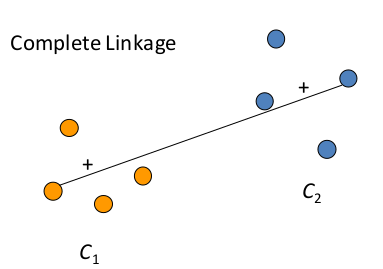
\includegraphics{img/complete.png}
\item
  \textbf{\emph{Single linkage}}. Dilakukan dengan menghitung jarak
  antara dua titik terdekat pada kedua \emph{cluster}.
  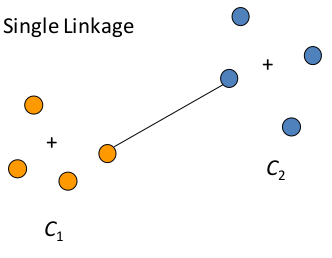
\includegraphics{img/single.png}
\item
  \textbf{\emph{Average linkage}}. Dilakukan dengan menghitung jarak
  rata-rata antara semua pasangan titik pada kedua cluster.
  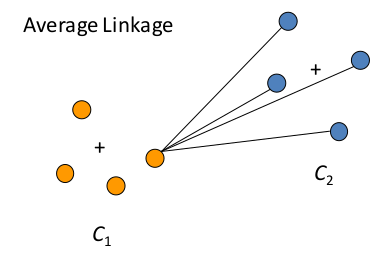
\includegraphics{img/average.png}
\item
  \textbf{\emph{Average-group linkage}}. Dilakukan dengan menghitung
  jarak antara \emph{centroid} dari kedua \emph{cluster}.
  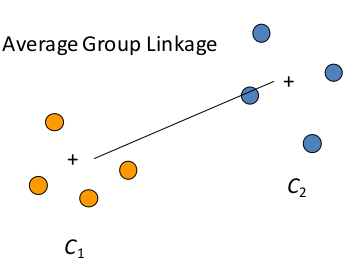
\includegraphics{img/average_group.png}
\end{enumerate}

Teknik penghitungan jarak juga beragam. Dalam implementasi ini,
diterapkan jarak \emph{manhattan}, \emph{euclidean}, dan \emph{cosine}.

    \subsection{Class}\label{class}

    \begin{Verbatim}[commandchars=\\\{\}]
{\color{incolor}In [{\color{incolor}3}]:} \PY{k+kn}{import} \PY{n+nn}{numpy} \PY{k}{as} \PY{n+nn}{np}
        \PY{k+kn}{import} \PY{n+nn}{math}
        
        \PY{k}{class} \PY{n+nc}{AgglomerativeClustering}\PY{p}{:}
            \PY{l+s+sd}{\PYZsq{}\PYZsq{}\PYZsq{}}
        \PY{l+s+sd}{    Kelas untuk mengakomodasi nilai metode agglomerative clustering}
        \PY{l+s+sd}{    \PYZsq{}\PYZsq{}\PYZsq{}}
            
            \PY{c+c1}{\PYZsh{} Nilai default parameter}
            \PY{n}{n\PYZus{}clusters} \PY{o}{=} \PY{l+m+mi}{2}
            \PY{n}{linkage} \PY{o}{=} \PY{l+s+s1}{\PYZsq{}}\PY{l+s+s1}{complete}\PY{l+s+s1}{\PYZsq{}}
            \PY{n}{metrics} \PY{o}{=} \PY{l+s+s1}{\PYZsq{}}\PY{l+s+s1}{euclidean}\PY{l+s+s1}{\PYZsq{}}
            
            \PY{n}{available\PYZus{}metrics} \PY{o}{=} \PY{p}{[}\PY{l+s+s1}{\PYZsq{}}\PY{l+s+s1}{euclidean}\PY{l+s+s1}{\PYZsq{}}\PY{p}{,} \PY{l+s+s1}{\PYZsq{}}\PY{l+s+s1}{manhattan}\PY{l+s+s1}{\PYZsq{}}\PY{p}{,} \PY{l+s+s1}{\PYZsq{}}\PY{l+s+s1}{cosine}\PY{l+s+s1}{\PYZsq{}}\PY{p}{]}
            \PY{n}{available\PYZus{}linkage} \PY{o}{=} \PY{p}{[}\PY{l+s+s1}{\PYZsq{}}\PY{l+s+s1}{complete}\PY{l+s+s1}{\PYZsq{}}\PY{p}{,} \PY{l+s+s1}{\PYZsq{}}\PY{l+s+s1}{single}\PY{l+s+s1}{\PYZsq{}}\PY{p}{,} \PY{l+s+s1}{\PYZsq{}}\PY{l+s+s1}{average\PYZus{}group}\PY{l+s+s1}{\PYZsq{}}\PY{p}{,} \PY{l+s+s1}{\PYZsq{}}\PY{l+s+s1}{average}\PY{l+s+s1}{\PYZsq{}}\PY{p}{]}
            
            \PY{k}{def} \PY{n+nf}{\PYZus{}\PYZus{}init\PYZus{}\PYZus{}}\PY{p}{(}\PY{n+nb+bp}{self}\PY{p}{,} \PY{n}{n\PYZus{}clusters}\PY{o}{=}\PY{n}{n\PYZus{}clusters}\PY{p}{,} \PY{n}{linkage}\PY{o}{=}\PY{n}{linkage}\PY{p}{,} \PY{n}{metrics}\PY{o}{=}\PY{n}{metrics}\PY{p}{)}\PY{p}{:}
                \PY{l+s+sd}{\PYZsq{}\PYZsq{}\PYZsq{}}
        \PY{l+s+sd}{        Inisiasi kelas. Parameter yang dibutuhkan untuk setiap kelas diinisiasi atau diisi dengan nilai default }
        \PY{l+s+sd}{        \PYZsq{}\PYZsq{}\PYZsq{}}
                \PY{k}{if} \PY{n}{n\PYZus{}clusters} \PY{o}{\PYZlt{}}\PY{o}{=} \PY{l+m+mi}{0}\PY{p}{:}
                    \PY{k}{raise} \PY{n+ne}{Exception}\PY{p}{(}\PY{l+s+s1}{\PYZsq{}}\PY{l+s+s1}{n\PYZus{}clusters must be higher than 0}\PY{l+s+s1}{\PYZsq{}}\PY{p}{)}
                \PY{k}{if} \PY{n}{metrics} \PY{o+ow}{not} \PY{o+ow}{in} \PY{n+nb+bp}{self}\PY{o}{.}\PY{n}{available\PYZus{}metrics}\PY{p}{:}
                    \PY{k}{raise} \PY{n+ne}{Exception}\PY{p}{(}\PY{l+s+s1}{\PYZsq{}}\PY{l+s+s1}{No metrics }\PY{l+s+se}{\PYZbs{}\PYZsq{}}\PY{l+s+s1}{\PYZsq{}} \PY{o}{+} \PY{n+nb}{str}\PY{p}{(}\PY{n}{metrics}\PY{p}{)} \PY{o}{+} \PY{l+s+s1}{\PYZsq{}}\PY{l+s+se}{\PYZbs{}\PYZsq{}}\PY{l+s+s1}{. Available metrics }\PY{l+s+s1}{\PYZsq{}}\PY{o}{+} \PY{n+nb}{str}\PY{p}{(}\PY{n+nb+bp}{self}\PY{o}{.}\PY{n}{available\PYZus{}metrics}\PY{p}{)}\PY{p}{)}
                \PY{k}{if} \PY{n}{linkage} \PY{o+ow}{not} \PY{o+ow}{in} \PY{n+nb+bp}{self}\PY{o}{.}\PY{n}{available\PYZus{}linkage}\PY{p}{:}
                    \PY{k}{raise} \PY{n+ne}{Exception}\PY{p}{(}\PY{l+s+s1}{\PYZsq{}}\PY{l+s+s1}{No linkage }\PY{l+s+se}{\PYZbs{}\PYZsq{}}\PY{l+s+s1}{\PYZsq{}} \PY{o}{+} \PY{n+nb}{str}\PY{p}{(}\PY{n}{linkage}\PY{p}{)} \PY{o}{+} \PY{l+s+s1}{\PYZsq{}}\PY{l+s+se}{\PYZbs{}\PYZsq{}}\PY{l+s+s1}{. Available linkage }\PY{l+s+s1}{\PYZsq{}}\PY{o}{+} \PY{n+nb}{str}\PY{p}{(}\PY{n+nb+bp}{self}\PY{o}{.}\PY{n}{available\PYZus{}linkage}\PY{p}{)}\PY{p}{)}
                \PY{n+nb+bp}{self}\PY{o}{.}\PY{n}{metrics} \PY{o}{=} \PY{n}{metrics}
                \PY{n+nb+bp}{self}\PY{o}{.}\PY{n}{n\PYZus{}clusters} \PY{o}{=} \PY{n}{n\PYZus{}clusters}
                \PY{n+nb+bp}{self}\PY{o}{.}\PY{n}{linkage} \PY{o}{=} \PY{n}{linkage}
                
            \PY{k}{def} \PY{n+nf}{\PYZus{}\PYZus{}euclidean\PYZus{}distance}\PY{p}{(}\PY{n+nb+bp}{self}\PY{p}{,} \PY{n}{data1}\PY{p}{,} \PY{n}{data2}\PY{p}{)}\PY{p}{:}
                \PY{l+s+sd}{\PYZsq{}\PYZsq{}\PYZsq{}}
        \PY{l+s+sd}{        Fungsi untuk menghitung euclidean distance di antara dua vector dengan panjang yang sama}
        \PY{l+s+sd}{        \PYZsq{}\PYZsq{}\PYZsq{}}
                \PY{n+nb}{sum} \PY{o}{=} \PY{l+m+mi}{0}
                \PY{k}{if} \PY{p}{(}\PY{n+nb}{len}\PY{p}{(}\PY{n}{data1}\PY{p}{)} \PY{o}{==} \PY{n+nb}{len}\PY{p}{(}\PY{n}{data2}\PY{p}{)}\PY{p}{)}\PY{p}{:}
                    \PY{k}{for} \PY{n}{x1}\PY{p}{,} \PY{n}{x2} \PY{o+ow}{in} \PY{n+nb}{zip}\PY{p}{(}\PY{n}{data1}\PY{p}{,} \PY{n}{data2}\PY{p}{)}\PY{p}{:}
                        \PY{n+nb}{sum} \PY{o}{+}\PY{o}{=} \PY{p}{(}\PY{n}{x1} \PY{o}{\PYZhy{}} \PY{n}{x2}\PY{p}{)}\PY{o}{*}\PY{o}{*}\PY{l+m+mi}{2}
                    \PY{n}{dist} \PY{o}{=} \PY{n}{math}\PY{o}{.}\PY{n}{sqrt}\PY{p}{(}\PY{n+nb}{sum}\PY{p}{)}
                    \PY{k}{return} \PY{n}{dist}
                \PY{k}{else}\PY{p}{:}
                    \PY{k}{raise} \PY{n+ne}{Exception}\PY{p}{(}\PY{l+s+s1}{\PYZsq{}}\PY{l+s+s1}{Length doesn}\PY{l+s+se}{\PYZbs{}\PYZsq{}}\PY{l+s+s1}{t match}\PY{l+s+s1}{\PYZsq{}}\PY{p}{)}
        
            \PY{k}{def} \PY{n+nf}{\PYZus{}\PYZus{}manhattan\PYZus{}distance}\PY{p}{(}\PY{n+nb+bp}{self}\PY{p}{,} \PY{n}{data1}\PY{p}{,} \PY{n}{data2}\PY{p}{)}\PY{p}{:}
                \PY{l+s+sd}{\PYZsq{}\PYZsq{}\PYZsq{}}
        \PY{l+s+sd}{        Fungsi untuk menghitung manhattan distance di antara dua vector dengan panjang yang sama}
        \PY{l+s+sd}{        \PYZsq{}\PYZsq{}\PYZsq{}}
                \PY{n+nb}{sum} \PY{o}{=} \PY{l+m+mi}{0}
                \PY{k}{if} \PY{p}{(}\PY{n+nb}{len}\PY{p}{(}\PY{n}{data1}\PY{p}{)} \PY{o}{==} \PY{n+nb}{len}\PY{p}{(}\PY{n}{data2}\PY{p}{)}\PY{p}{)}\PY{p}{:}
                    \PY{k}{for} \PY{n}{x1}\PY{p}{,} \PY{n}{x2} \PY{o+ow}{in} \PY{n+nb}{zip}\PY{p}{(}\PY{n}{data1}\PY{p}{,} \PY{n}{data2}\PY{p}{)}\PY{p}{:}
                        \PY{n+nb}{sum} \PY{o}{+}\PY{o}{=} \PY{n+nb}{abs}\PY{p}{(}\PY{n}{x1} \PY{o}{\PYZhy{}} \PY{n}{x2}\PY{p}{)}
                    \PY{k}{return} \PY{n+nb}{sum}
                \PY{k}{else}\PY{p}{:}
                    \PY{k}{raise} \PY{n+ne}{Exception}\PY{p}{(}\PY{l+s+s1}{\PYZsq{}}\PY{l+s+s1}{Length doesn}\PY{l+s+se}{\PYZbs{}\PYZsq{}}\PY{l+s+s1}{t match}\PY{l+s+s1}{\PYZsq{}}\PY{p}{)}
                    
            \PY{k}{def} \PY{n+nf}{\PYZus{}\PYZus{}cosine\PYZus{}distance}\PY{p}{(}\PY{n+nb+bp}{self}\PY{p}{,} \PY{n}{data1}\PY{p}{,} \PY{n}{data2}\PY{p}{)}\PY{p}{:}
                \PY{l+s+sd}{\PYZsq{}\PYZsq{}\PYZsq{}}
        \PY{l+s+sd}{        Fungsi untuk menghitung cosine distance di antara dua vector dengan panjang yang sama}
        \PY{l+s+sd}{        \PYZsq{}\PYZsq{}\PYZsq{}}
                \PY{k}{return} \PY{n}{np}\PY{o}{.}\PY{n}{dot}\PY{p}{(}\PY{n}{data1}\PY{p}{,} \PY{n}{data2}\PY{p}{)} \PY{o}{/} \PY{p}{(}\PY{n}{np}\PY{o}{.}\PY{n}{linalg}\PY{o}{.}\PY{n}{norm}\PY{p}{(}\PY{n}{data1}\PY{p}{)} \PY{o}{*} \PY{n}{np}\PY{o}{.}\PY{n}{linalg}\PY{o}{.}\PY{n}{norm}\PY{p}{(}\PY{n}{data2}\PY{p}{)}\PY{p}{)}
        
            \PY{k}{def} \PY{n+nf}{\PYZus{}\PYZus{}get\PYZus{}distance}\PY{p}{(}\PY{n+nb+bp}{self}\PY{p}{,} \PY{n}{data1}\PY{p}{,} \PY{n}{data2}\PY{p}{,} \PY{n}{metrics}\PY{p}{)}\PY{p}{:}
                \PY{l+s+sd}{\PYZsq{}\PYZsq{}\PYZsq{}}
        \PY{l+s+sd}{        Fungsi untuk menghitung jarak dua vector dengan metric pengukuran jarak yang telah ditentukan}
        \PY{l+s+sd}{        \PYZsq{}\PYZsq{}\PYZsq{}}
                \PY{k}{if} \PY{p}{(}\PY{n}{metrics} \PY{o}{==} \PY{l+s+s1}{\PYZsq{}}\PY{l+s+s1}{euclidean}\PY{l+s+s1}{\PYZsq{}}\PY{p}{)}\PY{p}{:}
                    \PY{n}{dist} \PY{o}{=} \PY{n+nb+bp}{self}\PY{o}{.}\PY{n}{\PYZus{}\PYZus{}euclidean\PYZus{}distance}\PY{p}{(}\PY{n}{data1}\PY{p}{,} \PY{n}{data2}\PY{p}{)}
                \PY{k}{elif} \PY{p}{(}\PY{n}{metrics} \PY{o}{==} \PY{l+s+s1}{\PYZsq{}}\PY{l+s+s1}{manhattan}\PY{l+s+s1}{\PYZsq{}}\PY{p}{)}\PY{p}{:}
                    \PY{n}{dist} \PY{o}{=} \PY{n+nb+bp}{self}\PY{o}{.}\PY{n}{\PYZus{}\PYZus{}manhattan\PYZus{}distance}\PY{p}{(}\PY{n}{data1}\PY{p}{,} \PY{n}{data2}\PY{p}{)}
                \PY{k}{elif} \PY{p}{(}\PY{n}{metrics} \PY{o}{==} \PY{l+s+s1}{\PYZsq{}}\PY{l+s+s1}{cosine}\PY{l+s+s1}{\PYZsq{}}\PY{p}{)}\PY{p}{:}
                    \PY{n}{dist} \PY{o}{=} \PY{n+nb+bp}{self}\PY{o}{.}\PY{n}{\PYZus{}\PYZus{}cosine\PYZus{}distance}\PY{p}{(}\PY{n}{data1}\PY{p}{,} \PY{n}{data2}\PY{p}{)}
                \PY{k}{else}\PY{p}{:}
                    \PY{k}{raise} \PY{n+ne}{Exception}\PY{p}{(}\PY{l+s+s1}{\PYZsq{}}\PY{l+s+s1}{Metrics not defined}\PY{l+s+s1}{\PYZsq{}}\PY{p}{)}
                \PY{k}{return} \PY{n}{dist}
            
            \PY{k}{def} \PY{n+nf}{\PYZus{}\PYZus{}complete\PYZus{}linkage}\PY{p}{(}\PY{n+nb+bp}{self}\PY{p}{,} \PY{n}{cluster1}\PY{p}{,} \PY{n}{cluster2}\PY{p}{,} \PY{n}{dist\PYZus{}matrix}\PY{p}{)}\PY{p}{:}
                \PY{l+s+sd}{\PYZsq{}\PYZsq{}\PYZsq{}}
        \PY{l+s+sd}{        Fungsi untuk menghitung jarak antara dua cluster dengan pendekatan complete linkage}
        \PY{l+s+sd}{        \PYZsq{}\PYZsq{}\PYZsq{}}
                \PY{n}{max\PYZus{}dist} \PY{o}{=} \PY{l+m+mi}{0}
                \PY{k}{for} \PY{n}{v1} \PY{o+ow}{in} \PY{n}{cluster1}\PY{p}{:}
                    \PY{k}{for} \PY{n}{v2} \PY{o+ow}{in} \PY{n}{cluster2}\PY{p}{:}
                        \PY{k}{if} \PY{p}{(}\PY{n}{max\PYZus{}dist} \PY{o}{\PYZlt{}} \PY{n}{dist\PYZus{}matrix}\PY{p}{[}\PY{n}{v1}\PY{p}{]}\PY{p}{[}\PY{n}{v2}\PY{p}{]}\PY{p}{)}\PY{p}{:}
                            \PY{n}{max\PYZus{}dist} \PY{o}{=} \PY{n}{dist\PYZus{}matrix}\PY{p}{[}\PY{n}{v1}\PY{p}{]}\PY{p}{[}\PY{n}{v2}\PY{p}{]}
                \PY{k}{return} \PY{n}{max\PYZus{}dist}
        
            \PY{k}{def} \PY{n+nf}{\PYZus{}\PYZus{}single\PYZus{}linkage}\PY{p}{(}\PY{n+nb+bp}{self}\PY{p}{,} \PY{n}{cluster1}\PY{p}{,} \PY{n}{cluster2}\PY{p}{,} \PY{n}{dist\PYZus{}matrix}\PY{p}{)}\PY{p}{:}
                \PY{l+s+sd}{\PYZsq{}\PYZsq{}\PYZsq{}}
        \PY{l+s+sd}{        Fungsi untuk menghitung jarak antara dua cluster dengan pendekatan single linkage}
        \PY{l+s+sd}{        \PYZsq{}\PYZsq{}\PYZsq{}}
                \PY{n}{min\PYZus{}dist} \PY{o}{=} \PY{k+kc}{None}
                \PY{k}{for} \PY{n}{v1} \PY{o+ow}{in} \PY{n}{cluster1}\PY{p}{:}
                    \PY{k}{for} \PY{n}{v2} \PY{o+ow}{in} \PY{n}{cluster2}\PY{p}{:}
                        \PY{k}{if} \PY{p}{(}\PY{n}{min\PYZus{}dist} \PY{o+ow}{is} \PY{k+kc}{None}\PY{p}{)} \PY{o+ow}{or} \PY{p}{(}\PY{n}{min\PYZus{}dist} \PY{o}{\PYZgt{}} \PY{n}{dist\PYZus{}matrix}\PY{p}{[}\PY{n}{v1}\PY{p}{]}\PY{p}{[}\PY{n}{v2}\PY{p}{]}\PY{p}{)}\PY{p}{:}
                            \PY{n}{min\PYZus{}dist} \PY{o}{=} \PY{n}{dist\PYZus{}matrix}\PY{p}{[}\PY{n}{v1}\PY{p}{]}\PY{p}{[}\PY{n}{v2}\PY{p}{]}
                \PY{k}{return} \PY{n}{min\PYZus{}dist}
        
            \PY{k}{def} \PY{n+nf}{\PYZus{}\PYZus{}average\PYZus{}linkage}\PY{p}{(}\PY{n+nb+bp}{self}\PY{p}{,} \PY{n}{cluster1}\PY{p}{,} \PY{n}{cluster2}\PY{p}{,} \PY{n}{dist\PYZus{}matrix}\PY{p}{)}\PY{p}{:}
                \PY{l+s+sd}{\PYZsq{}\PYZsq{}\PYZsq{}}
        \PY{l+s+sd}{        Fungsi untuk menghitung jarak antara dua cluster dengan pendekatan average linkage}
        \PY{l+s+sd}{        \PYZsq{}\PYZsq{}\PYZsq{}}
                \PY{n}{sum\PYZus{}dist} \PY{o}{=} \PY{l+m+mi}{0}
                \PY{n}{count\PYZus{}dist} \PY{o}{=} \PY{l+m+mi}{0}
                \PY{k}{for} \PY{n}{v1} \PY{o+ow}{in} \PY{n}{cluster1}\PY{p}{:}
                    \PY{k}{for} \PY{n}{v2} \PY{o+ow}{in} \PY{n}{cluster2}\PY{p}{:}
                        \PY{n}{sum\PYZus{}dist} \PY{o}{+}\PY{o}{=} \PY{n}{dist\PYZus{}matrix}\PY{p}{[}\PY{n}{v1}\PY{p}{]}\PY{p}{[}\PY{n}{v2}\PY{p}{]}
                        \PY{n}{count\PYZus{}dist} \PY{o}{+}\PY{o}{=} \PY{l+m+mi}{1}
                \PY{k}{return} \PY{n+nb}{float}\PY{p}{(}\PY{n}{sum\PYZus{}dist}\PY{p}{)}\PY{o}{/}\PY{n+nb}{float}\PY{p}{(}\PY{n}{count\PYZus{}dist}\PY{p}{)}
        
            \PY{k}{def} \PY{n+nf}{\PYZus{}\PYZus{}group\PYZus{}average\PYZus{}linkage}\PY{p}{(}\PY{n+nb+bp}{self}\PY{p}{,} \PY{n}{cluster1}\PY{p}{,} \PY{n}{cluster2}\PY{p}{,} \PY{n}{data}\PY{p}{,} \PY{n}{distance}\PY{p}{)}\PY{p}{:}
                \PY{l+s+sd}{\PYZsq{}\PYZsq{}\PYZsq{}}
        \PY{l+s+sd}{        Fungsi untuk menghitung jarak antara dua cluster dengan pendekatan average group linkage}
        \PY{l+s+sd}{        \PYZsq{}\PYZsq{}\PYZsq{}}
                \PY{n}{data1} \PY{o}{=} \PY{p}{[}\PY{n}{data}\PY{p}{[}\PY{n}{i}\PY{p}{]} \PY{k}{for} \PY{n}{i} \PY{o+ow}{in} \PY{n}{cluster1}\PY{p}{]}
                \PY{n}{data2} \PY{o}{=} \PY{p}{[}\PY{n}{data}\PY{p}{[}\PY{n}{i}\PY{p}{]} \PY{k}{for} \PY{n}{i} \PY{o+ow}{in} \PY{n}{cluster2}\PY{p}{]}
        
                \PY{n}{avg1} \PY{o}{=} \PY{n}{np}\PY{o}{.}\PY{n}{mean}\PY{p}{(}\PY{n}{data1}\PY{p}{,} \PY{n}{axis} \PY{o}{=} \PY{l+m+mi}{0}\PY{p}{)}
                \PY{n}{avg2} \PY{o}{=} \PY{n}{np}\PY{o}{.}\PY{n}{mean}\PY{p}{(}\PY{n}{data2}\PY{p}{,} \PY{n}{axis} \PY{o}{=} \PY{l+m+mi}{0}\PY{p}{)}
        
                \PY{k}{return} \PY{n+nb+bp}{self}\PY{o}{.}\PY{n}{\PYZus{}\PYZus{}get\PYZus{}distance}\PY{p}{(}\PY{n}{avg1}\PY{p}{,} \PY{n}{avg2}\PY{p}{,} \PY{n}{distance}\PY{p}{)}
            
            \PY{k}{def} \PY{n+nf}{\PYZus{}\PYZus{}calculate\PYZus{}distance\PYZus{}matrix}\PY{p}{(}\PY{n+nb+bp}{self}\PY{p}{,} \PY{n}{data}\PY{p}{,} \PY{n}{metrics}\PY{p}{)}\PY{p}{:}
                \PY{l+s+sd}{\PYZsq{}\PYZsq{}\PYZsq{}}
        \PY{l+s+sd}{        Fungsi untuk menghitung distance matrix untuk semua pasangan vector di dalam data}
        \PY{l+s+sd}{        \PYZsq{}\PYZsq{}\PYZsq{}}
                \PY{n}{dist\PYZus{}matrix} \PY{o}{=} \PY{p}{[}\PY{p}{]}
                \PY{k}{for} \PY{n}{idx1}\PY{p}{,} \PY{n}{data1} \PY{o+ow}{in} \PY{n+nb}{enumerate}\PY{p}{(}\PY{n}{data}\PY{p}{)}\PY{p}{:}
                    \PY{n}{curr\PYZus{}dist\PYZus{}matrix} \PY{o}{=} \PY{p}{[}\PY{p}{]}
                    \PY{k}{for} \PY{n}{idx2}\PY{p}{,} \PY{n}{data2} \PY{o+ow}{in} \PY{n+nb}{enumerate}\PY{p}{(}\PY{n}{data}\PY{p}{)}\PY{p}{:}
                        \PY{k}{if} \PY{p}{(}\PY{n}{idx1} \PY{o}{\PYZgt{}} \PY{n}{idx2}\PY{p}{)}\PY{p}{:}
                            \PY{n}{curr\PYZus{}dist\PYZus{}matrix}\PY{o}{.}\PY{n}{append}\PY{p}{(}\PY{n}{dist\PYZus{}matrix}\PY{p}{[}\PY{n}{idx2}\PY{p}{]}\PY{p}{[}\PY{n}{idx1}\PY{p}{]}\PY{p}{)}
                        \PY{k}{else}\PY{p}{:}
                            \PY{n}{dist} \PY{o}{=} \PY{n+nb+bp}{self}\PY{o}{.}\PY{n}{\PYZus{}\PYZus{}get\PYZus{}distance}\PY{p}{(}\PY{n}{data1}\PY{p}{,} \PY{n}{data2}\PY{p}{,} \PY{n}{metrics}\PY{p}{)}
                            \PY{n}{curr\PYZus{}dist\PYZus{}matrix}\PY{o}{.}\PY{n}{append}\PY{p}{(}\PY{n}{dist}\PY{p}{)}
                    \PY{n}{dist\PYZus{}matrix}\PY{o}{.}\PY{n}{append}\PY{p}{(}\PY{n}{curr\PYZus{}dist\PYZus{}matrix}\PY{p}{)}
                \PY{k}{return} \PY{n}{dist\PYZus{}matrix}
                
            \PY{k}{def} \PY{n+nf}{fit\PYZus{}predict}\PY{p}{(}\PY{n+nb+bp}{self}\PY{p}{,} \PY{n}{data}\PY{p}{)}\PY{p}{:}
                \PY{l+s+sd}{\PYZsq{}\PYZsq{}\PYZsq{}}
        \PY{l+s+sd}{        Fungsi untuk melakukan clustering secara agglomerative}
        \PY{l+s+sd}{        \PYZsq{}\PYZsq{}\PYZsq{}}
                
                \PY{c+c1}{\PYZsh{} preprocessing distance matrix}
                \PY{k}{if} \PY{p}{(}\PY{n+nb+bp}{self}\PY{o}{.}\PY{n}{linkage} \PY{o}{!=} \PY{l+s+s1}{\PYZsq{}}\PY{l+s+s1}{average\PYZus{}group}\PY{l+s+s1}{\PYZsq{}}\PY{p}{)}\PY{p}{:}
                    \PY{n}{dist\PYZus{}matrix} \PY{o}{=} \PY{n+nb+bp}{self}\PY{o}{.}\PY{n}{\PYZus{}\PYZus{}calculate\PYZus{}distance\PYZus{}matrix}\PY{p}{(}\PY{n}{data}\PY{p}{,} \PY{n+nb+bp}{self}\PY{o}{.}\PY{n}{metrics}\PY{p}{)}
                \PY{c+c1}{\PYZsh{} inisiasi cluster dengan satu elemen per cluster awal }
                \PY{n}{clusters} \PY{o}{=} \PY{p}{[}\PY{p}{[}\PY{n}{i}\PY{p}{]} \PY{k}{for} \PY{n}{i}\PY{p}{,} \PY{n}{c} \PY{o+ow}{in} \PY{n+nb}{enumerate}\PY{p}{(}\PY{n}{data}\PY{p}{)}\PY{p}{]}
        
                \PY{c+c1}{\PYZsh{} melakukan iterasi hingga diperoleh jumlah cluster sesuai yang dikehendaki}
                \PY{k}{while}\PY{p}{(}\PY{n+nb}{len}\PY{p}{(}\PY{n}{clusters}\PY{p}{)} \PY{o}{\PYZgt{}} \PY{n+nb+bp}{self}\PY{o}{.}\PY{n}{n\PYZus{}clusters}\PY{p}{)}\PY{p}{:}
                    \PY{n}{min\PYZus{}dist} \PY{o}{=} \PY{k+kc}{None}
                    \PY{n}{merge\PYZus{}pair} \PY{o}{=} \PY{p}{(}\PY{l+m+mi}{0}\PY{p}{,} \PY{l+m+mi}{0}\PY{p}{)}
                    
                    \PY{c+c1}{\PYZsh{} mencari cluster dengan jarak terdekat untuk di\PYZhy{}merge}
                    \PY{k}{for} \PY{n}{idx1}\PY{p}{,} \PY{n}{c1} \PY{o+ow}{in} \PY{n+nb}{enumerate}\PY{p}{(}\PY{n}{clusters}\PY{p}{)}\PY{p}{:}
                        \PY{k}{for} \PY{n}{idx2}\PY{p}{,} \PY{n}{c2} \PY{o+ow}{in} \PY{n+nb}{enumerate}\PY{p}{(}\PY{n}{clusters}\PY{p}{[}\PY{p}{(}\PY{n}{idx1} \PY{o}{+} \PY{l+m+mi}{1}\PY{p}{)} \PY{p}{:}\PY{p}{]}\PY{p}{)}\PY{p}{:}
                            \PY{k}{if} \PY{p}{(}\PY{n+nb+bp}{self}\PY{o}{.}\PY{n}{linkage} \PY{o}{==} \PY{l+s+s1}{\PYZsq{}}\PY{l+s+s1}{single}\PY{l+s+s1}{\PYZsq{}}\PY{p}{)}\PY{p}{:}
                                \PY{n}{dist} \PY{o}{=} \PY{n+nb+bp}{self}\PY{o}{.}\PY{n}{\PYZus{}\PYZus{}single\PYZus{}linkage}\PY{p}{(}\PY{n}{c1}\PY{p}{,} \PY{n}{c2}\PY{p}{,} \PY{n}{dist\PYZus{}matrix}\PY{p}{)}
                            \PY{k}{elif} \PY{p}{(}\PY{n+nb+bp}{self}\PY{o}{.}\PY{n}{linkage} \PY{o}{==} \PY{l+s+s1}{\PYZsq{}}\PY{l+s+s1}{complete}\PY{l+s+s1}{\PYZsq{}}\PY{p}{)}\PY{p}{:}
                                \PY{n}{dist} \PY{o}{=} \PY{n+nb+bp}{self}\PY{o}{.}\PY{n}{\PYZus{}\PYZus{}complete\PYZus{}linkage}\PY{p}{(}\PY{n}{c1}\PY{p}{,} \PY{n}{c2}\PY{p}{,} \PY{n}{dist\PYZus{}matrix}\PY{p}{)}
                            \PY{k}{elif} \PY{p}{(}\PY{n+nb+bp}{self}\PY{o}{.}\PY{n}{linkage} \PY{o}{==} \PY{l+s+s1}{\PYZsq{}}\PY{l+s+s1}{average}\PY{l+s+s1}{\PYZsq{}}\PY{p}{)}\PY{p}{:}
                                \PY{n}{dist} \PY{o}{=} \PY{n+nb+bp}{self}\PY{o}{.}\PY{n}{\PYZus{}\PYZus{}average\PYZus{}linkage}\PY{p}{(}\PY{n}{c1}\PY{p}{,} \PY{n}{c2}\PY{p}{,} \PY{n}{dist\PYZus{}matrix}\PY{p}{)}
                            \PY{k}{elif} \PY{p}{(}\PY{n+nb+bp}{self}\PY{o}{.}\PY{n}{linkage} \PY{o}{==} \PY{l+s+s1}{\PYZsq{}}\PY{l+s+s1}{average\PYZus{}group}\PY{l+s+s1}{\PYZsq{}}\PY{p}{)}\PY{p}{:}
                                \PY{n}{dist} \PY{o}{=} \PY{n+nb+bp}{self}\PY{o}{.}\PY{n}{\PYZus{}\PYZus{}group\PYZus{}average\PYZus{}linkage}\PY{p}{(}\PY{n}{c1}\PY{p}{,} \PY{n}{c2}\PY{p}{,} \PY{n}{data}\PY{p}{,} \PY{n+nb+bp}{self}\PY{o}{.}\PY{n}{metrics}\PY{p}{)}
                            \PY{k}{else}\PY{p}{:}
                                \PY{k}{raise} \PY{n+ne}{Exception}\PY{p}{(}\PY{l+s+s1}{\PYZsq{}}\PY{l+s+s1}{Linkage not defined}\PY{l+s+s1}{\PYZsq{}}\PY{p}{)}
                            \PY{k}{if} \PY{p}{(}\PY{n}{min\PYZus{}dist} \PY{o}{==} \PY{k+kc}{None}\PY{p}{)} \PY{o+ow}{or} \PY{p}{(}\PY{n}{dist} \PY{o}{\PYZlt{}} \PY{n}{min\PYZus{}dist}\PY{p}{)}\PY{p}{:}
                                \PY{n}{min\PYZus{}dist} \PY{o}{=} \PY{n}{dist}
                                \PY{n}{merge\PYZus{}pair} \PY{o}{=} \PY{p}{(}\PY{n}{idx1}\PY{p}{,} \PY{n}{idx1} \PY{o}{+} \PY{l+m+mi}{1} \PY{o}{+} \PY{n}{idx2}\PY{p}{)}
                    
                    \PY{c+c1}{\PYZsh{} merge pasangan cluster dengan jarak terdekat}
                    \PY{n}{result\PYZus{}cluster} \PY{o}{=} \PY{p}{[}\PY{p}{]}
                    \PY{k}{for} \PY{n}{idx}\PY{p}{,} \PY{n}{c} \PY{o+ow}{in} \PY{n+nb}{enumerate}\PY{p}{(}\PY{n}{clusters}\PY{p}{)}\PY{p}{:}
                        \PY{k}{if} \PY{n}{idx} \PY{o+ow}{not} \PY{o+ow}{in} \PY{n}{merge\PYZus{}pair}\PY{p}{:}
                            \PY{n}{result\PYZus{}cluster}\PY{o}{.}\PY{n}{append}\PY{p}{(}\PY{n}{c}\PY{p}{)}
        
                    \PY{n}{result\PYZus{}cluster}\PY{o}{.}\PY{n}{append}\PY{p}{(}\PY{n}{clusters}\PY{p}{[}\PY{n}{merge\PYZus{}pair}\PY{p}{[}\PY{l+m+mi}{0}\PY{p}{]}\PY{p}{]} \PY{o}{+} \PY{n}{clusters}\PY{p}{[}\PY{n}{merge\PYZus{}pair}\PY{p}{[}\PY{l+m+mi}{1}\PY{p}{]}\PY{p}{]}\PY{p}{)}
        
                    \PY{n}{clusters} \PY{o}{=} \PY{n}{result\PYZus{}cluster}
        
                \PY{c+c1}{\PYZsh{} menampilkan hasil clustering}
                \PY{n}{result\PYZus{}per\PYZus{}item} \PY{o}{=} \PY{n}{np}\PY{o}{.}\PY{n}{full}\PY{p}{(}\PY{n+nb}{len}\PY{p}{(}\PY{n}{data}\PY{p}{)}\PY{p}{,} \PY{l+m+mi}{0}\PY{p}{)}
                \PY{k}{for} \PY{n}{idx}\PY{p}{,} \PY{n}{clust} \PY{o+ow}{in} \PY{n+nb}{enumerate}\PY{p}{(}\PY{n}{clusters}\PY{p}{)}\PY{p}{:}
                    \PY{n}{result\PYZus{}per\PYZus{}item}\PY{p}{[}\PY{n}{clust}\PY{p}{]} \PY{o}{=} \PY{n}{idx}
        
                \PY{k}{return} \PY{n}{result\PYZus{}per\PYZus{}item}
            
            \PY{l+s+sd}{\PYZsq{}\PYZsq{}\PYZsq{}}
        \PY{l+s+sd}{    Getter untuk parameter}
        \PY{l+s+sd}{    \PYZsq{}\PYZsq{}\PYZsq{}}
            \PY{k}{def} \PY{n+nf}{get\PYZus{}n\PYZus{}cluster}\PY{p}{(}\PY{n+nb+bp}{self}\PY{p}{)}\PY{p}{:}
                \PY{k}{return} \PY{n+nb+bp}{self}\PY{o}{.}\PY{n}{n\PYZus{}clusters}
            
            \PY{k}{def} \PY{n+nf}{get\PYZus{}linkage}\PY{p}{(}\PY{n+nb+bp}{self}\PY{p}{)}\PY{p}{:}
                \PY{k}{return} \PY{n+nb+bp}{self}\PY{o}{.}\PY{n}{linkage}
            
            \PY{k}{def} \PY{n+nf}{get\PYZus{}metrics}\PY{p}{(}\PY{n+nb+bp}{self}\PY{p}{)}\PY{p}{:}
                \PY{k}{return} \PY{n+nb+bp}{self}\PY{o}{.}\PY{n}{metrics}
\end{Verbatim}


    \subsection{Experiments}\label{experiments}

Berikut adalah eksperimen yang dilakukan untuk melakukan
\emph{clustering} terhadap \emph{dataset} iris. Digunakan
\emph{euclidean distance} dan berbagai variasi perhitungan
\emph{linkage} antara dua cluster untuk menerapkan metode
\emph{agglomerative clustering}.

    \begin{Verbatim}[commandchars=\\\{\}]
{\color{incolor}In [{\color{incolor}4}]:} \PY{n}{iris} \PY{o}{=} \PY{n}{datasets}\PY{o}{.}\PY{n}{load\PYZus{}iris}\PY{p}{(}\PY{p}{)}
        \PY{n}{data} \PY{o}{=} \PY{n}{iris}\PY{o}{.}\PY{n}{data}
        \PY{n}{label} \PY{o}{=} \PY{n}{iris}\PY{o}{.}\PY{n}{target}
\end{Verbatim}


    \paragraph{Clustering dengan Complete
Linkage}\label{clustering-dengan-complete-linkage}

Pada percobaan ini, digunakan pendekatan \emph{complete linkage} untuk
menghitung jarak antar pasangan cluster. Hasil clustering dan
\emph{purity}-nya dapat dilihat pada \emph{output} dari eksekusi
\emph{code}.

    \begin{Verbatim}[commandchars=\\\{\}]
{\color{incolor}In [{\color{incolor}5}]:} \PY{n}{aglo} \PY{o}{=} \PY{n}{AgglomerativeClustering}\PY{p}{(}\PY{n}{n\PYZus{}clusters}\PY{o}{=}\PY{l+m+mi}{3}\PY{p}{,} \PY{n}{linkage}\PY{o}{=}\PY{l+s+s1}{\PYZsq{}}\PY{l+s+s1}{complete}\PY{l+s+s1}{\PYZsq{}}\PY{p}{,} \PY{n}{metrics}\PY{o}{=}\PY{l+s+s1}{\PYZsq{}}\PY{l+s+s1}{euclidean}\PY{l+s+s1}{\PYZsq{}}\PY{p}{)}
        \PY{n}{start} \PY{o}{=} \PY{n}{time}\PY{o}{.}\PY{n}{time}\PY{p}{(}\PY{p}{)}
        \PY{n}{pred} \PY{o}{=} \PY{n}{aglo}\PY{o}{.}\PY{n}{fit\PYZus{}predict}\PY{p}{(}\PY{n}{data}\PY{p}{)}
        
        \PY{n+nb}{print}\PY{p}{(}\PY{l+s+s2}{\PYZdq{}}\PY{l+s+s2}{\PYZhy{}\PYZhy{}\PYZhy{}\PYZhy{} Time taken: }\PY{l+s+si}{\PYZob{}\PYZcb{}}\PY{l+s+s2}{ s \PYZhy{}\PYZhy{}\PYZhy{}\PYZhy{}}\PY{l+s+s2}{\PYZdq{}}\PY{o}{.}\PY{n}{format}\PY{p}{(}\PY{n}{time}\PY{o}{.}\PY{n}{time}\PY{p}{(}\PY{p}{)} \PY{o}{\PYZhy{}} \PY{n}{start}\PY{p}{)}\PY{p}{)}
        \PY{n+nb}{print}\PY{p}{(}\PY{l+s+s2}{\PYZdq{}}\PY{l+s+s2}{Cluster prediction:}\PY{l+s+s2}{\PYZdq{}}\PY{p}{)}
        \PY{n+nb}{print}\PY{p}{(}\PY{n}{pred}\PY{p}{)}
        \PY{n+nb}{print}\PY{p}{(}\PY{l+s+s2}{\PYZdq{}}\PY{l+s+s2}{Purity: }\PY{l+s+si}{\PYZob{}\PYZcb{}}\PY{l+s+s2}{\PYZdq{}}\PY{o}{.}\PY{n}{format}\PY{p}{(}\PY{n}{purity}\PY{p}{(}\PY{n}{pred}\PY{p}{,} \PY{n}{label}\PY{p}{)}\PY{p}{)}\PY{p}{)}
\end{Verbatim}


    \begin{Verbatim}[commandchars=\\\{\}]
---- Time taken: 0.8769066333770752 s ----
Cluster prediction:
[1 1 1 1 1 1 1 1 1 1 1 1 1 1 1 1 1 1 1 1 1 1 1 1 1 1 1 1 1 1 1 1 1 1 1 1 1
 1 1 1 1 1 1 1 1 1 1 1 1 1 2 2 2 0 2 0 2 0 2 0 0 0 0 2 0 2 0 0 2 0 2 0 2 2
 2 2 2 2 2 0 0 0 0 2 0 2 2 2 0 0 0 2 0 0 0 0 0 2 0 0 2 2 2 2 2 2 0 2 2 2 2
 2 2 2 2 2 2 2 2 2 2 2 2 2 2 2 2 2 2 2 2 2 2 2 2 2 2 2 2 2 2 2 2 2 2 2 2 2
 2 2]
Purity: 0.84

    \end{Verbatim}

    \paragraph{Clustering dengan Single
Linkage}\label{clustering-dengan-single-linkage}

Pada percobaan ini, digunakan pendekatan \emph{single linkage} untuk
menghitung jarak antar pasangan cluster. Hasil clustering dan
\emph{purity}-nya dapat dilihat pada \emph{output} dari eksekusi
\emph{code}.

    \begin{Verbatim}[commandchars=\\\{\}]
{\color{incolor}In [{\color{incolor}6}]:} \PY{n}{aglo} \PY{o}{=} \PY{n}{AgglomerativeClustering}\PY{p}{(}\PY{n}{n\PYZus{}clusters}\PY{o}{=}\PY{l+m+mi}{3}\PY{p}{,} \PY{n}{linkage}\PY{o}{=}\PY{l+s+s1}{\PYZsq{}}\PY{l+s+s1}{single}\PY{l+s+s1}{\PYZsq{}}\PY{p}{,} \PY{n}{metrics}\PY{o}{=}\PY{l+s+s1}{\PYZsq{}}\PY{l+s+s1}{euclidean}\PY{l+s+s1}{\PYZsq{}}\PY{p}{)}
        \PY{n}{start} \PY{o}{=} \PY{n}{time}\PY{o}{.}\PY{n}{time}\PY{p}{(}\PY{p}{)}
        \PY{n}{pred} \PY{o}{=} \PY{n}{aglo}\PY{o}{.}\PY{n}{fit\PYZus{}predict}\PY{p}{(}\PY{n}{data}\PY{p}{)}
        
        \PY{n+nb}{print}\PY{p}{(}\PY{l+s+s2}{\PYZdq{}}\PY{l+s+s2}{\PYZhy{}\PYZhy{}\PYZhy{}\PYZhy{} Time taken: }\PY{l+s+si}{\PYZob{}\PYZcb{}}\PY{l+s+s2}{ s \PYZhy{}\PYZhy{}\PYZhy{}\PYZhy{}}\PY{l+s+s2}{\PYZdq{}}\PY{o}{.}\PY{n}{format}\PY{p}{(}\PY{n}{time}\PY{o}{.}\PY{n}{time}\PY{p}{(}\PY{p}{)} \PY{o}{\PYZhy{}} \PY{n}{start}\PY{p}{)}\PY{p}{)}
        \PY{n+nb}{print}\PY{p}{(}\PY{l+s+s2}{\PYZdq{}}\PY{l+s+s2}{Cluster prediction:}\PY{l+s+s2}{\PYZdq{}}\PY{p}{)}
        \PY{n+nb}{print}\PY{p}{(}\PY{n}{pred}\PY{p}{)}
        \PY{n+nb}{print}\PY{p}{(}\PY{l+s+s2}{\PYZdq{}}\PY{l+s+s2}{Purity: }\PY{l+s+si}{\PYZob{}\PYZcb{}}\PY{l+s+s2}{\PYZdq{}}\PY{o}{.}\PY{n}{format}\PY{p}{(}\PY{n}{purity}\PY{p}{(}\PY{n}{pred}\PY{p}{,} \PY{n}{label}\PY{p}{)}\PY{p}{)}\PY{p}{)}
\end{Verbatim}


    \begin{Verbatim}[commandchars=\\\{\}]
---- Time taken: 0.7279071807861328 s ----
Cluster prediction:
[1 1 1 1 1 1 1 1 1 1 1 1 1 1 1 1 1 1 1 1 1 1 1 1 1 1 1 1 1 1 1 1 1 1 1 1 1
 1 1 1 1 1 1 1 1 1 1 1 1 1 2 2 2 2 2 2 2 2 2 2 2 2 2 2 2 2 2 2 2 2 2 2 2 2
 2 2 2 2 2 2 2 2 2 2 2 2 2 2 2 2 2 2 2 2 2 2 2 2 2 2 2 2 2 2 2 2 2 2 2 2 2
 2 2 2 2 2 2 0 2 2 2 2 2 2 2 2 2 2 2 2 2 0 2 2 2 2 2 2 2 2 2 2 2 2 2 2 2 2
 2 2]
Purity: 0.68

    \end{Verbatim}

    \paragraph{Clustering dengan Average
Linkage}\label{clustering-dengan-average-linkage}

Pada percobaan ini, digunakan pendekatan \emph{complete linkage} untuk
menghitung jarak antar pasangan cluster. Hasil clustering dan
\emph{purity}-nya dapat dilihat pada \emph{output} dari eksekusi
\emph{code}.

    \begin{Verbatim}[commandchars=\\\{\}]
{\color{incolor}In [{\color{incolor}7}]:} \PY{n}{aglo} \PY{o}{=} \PY{n}{AgglomerativeClustering}\PY{p}{(}\PY{n}{n\PYZus{}clusters}\PY{o}{=}\PY{l+m+mi}{3}\PY{p}{,} \PY{n}{linkage}\PY{o}{=}\PY{l+s+s1}{\PYZsq{}}\PY{l+s+s1}{average}\PY{l+s+s1}{\PYZsq{}}\PY{p}{,} \PY{n}{metrics}\PY{o}{=}\PY{l+s+s1}{\PYZsq{}}\PY{l+s+s1}{euclidean}\PY{l+s+s1}{\PYZsq{}}\PY{p}{)}
        \PY{n}{start} \PY{o}{=} \PY{n}{time}\PY{o}{.}\PY{n}{time}\PY{p}{(}\PY{p}{)}
        \PY{n}{pred} \PY{o}{=} \PY{n}{aglo}\PY{o}{.}\PY{n}{fit\PYZus{}predict}\PY{p}{(}\PY{n}{data}\PY{p}{)}
        
        \PY{n+nb}{print}\PY{p}{(}\PY{l+s+s2}{\PYZdq{}}\PY{l+s+s2}{\PYZhy{}\PYZhy{}\PYZhy{}\PYZhy{} Time taken: }\PY{l+s+si}{\PYZob{}\PYZcb{}}\PY{l+s+s2}{ s \PYZhy{}\PYZhy{}\PYZhy{}\PYZhy{}}\PY{l+s+s2}{\PYZdq{}}\PY{o}{.}\PY{n}{format}\PY{p}{(}\PY{n}{time}\PY{o}{.}\PY{n}{time}\PY{p}{(}\PY{p}{)} \PY{o}{\PYZhy{}} \PY{n}{start}\PY{p}{)}\PY{p}{)}
        \PY{n+nb}{print}\PY{p}{(}\PY{l+s+s2}{\PYZdq{}}\PY{l+s+s2}{Cluster prediction:}\PY{l+s+s2}{\PYZdq{}}\PY{p}{)}
        \PY{n+nb}{print}\PY{p}{(}\PY{n}{pred}\PY{p}{)}
        \PY{n+nb}{print}\PY{p}{(}\PY{l+s+s2}{\PYZdq{}}\PY{l+s+s2}{Purity: }\PY{l+s+si}{\PYZob{}\PYZcb{}}\PY{l+s+s2}{\PYZdq{}}\PY{o}{.}\PY{n}{format}\PY{p}{(}\PY{n}{purity}\PY{p}{(}\PY{n}{pred}\PY{p}{,} \PY{n}{label}\PY{p}{)}\PY{p}{)}\PY{p}{)}
\end{Verbatim}


    \begin{Verbatim}[commandchars=\\\{\}]
---- Time taken: 1.2760462760925293 s ----
Cluster prediction:
[0 0 0 0 0 0 0 0 0 0 0 0 0 0 0 0 0 0 0 0 0 0 0 0 0 0 0 0 0 0 0 0 0 0 0 0 0
 0 0 0 0 0 0 0 0 0 0 0 0 0 2 2 2 2 2 2 2 2 2 2 2 2 2 2 2 2 2 2 2 2 2 2 2 2
 2 2 2 2 2 2 2 2 2 2 2 2 2 2 2 2 2 2 2 2 2 2 2 2 2 2 1 2 1 1 1 1 2 1 1 1 1
 1 1 2 2 1 1 1 1 2 1 2 1 2 1 1 2 2 1 1 1 1 1 2 1 1 1 1 2 1 1 1 2 1 1 1 2 1
 1 2]
Purity: 0.9066666666666666

    \end{Verbatim}

    \paragraph{Clustering dengan Average-group
Linkage}\label{clustering-dengan-average-group-linkage}

Pada percobaan ini, digunakan pendekatan \emph{average-group linkage}
untuk menghitung jarak antar pasangan cluster. Hasil clustering dan
\emph{purity}-nya dapat dilihat pada \emph{output} dari eksekusi
\emph{code}.

    \begin{Verbatim}[commandchars=\\\{\}]
{\color{incolor}In [{\color{incolor}8}]:} \PY{n}{aglo} \PY{o}{=} \PY{n}{AgglomerativeClustering}\PY{p}{(}\PY{n}{n\PYZus{}clusters}\PY{o}{=}\PY{l+m+mi}{3}\PY{p}{,} \PY{n}{linkage}\PY{o}{=}\PY{l+s+s1}{\PYZsq{}}\PY{l+s+s1}{average\PYZus{}group}\PY{l+s+s1}{\PYZsq{}}\PY{p}{,} \PY{n}{metrics}\PY{o}{=}\PY{l+s+s1}{\PYZsq{}}\PY{l+s+s1}{euclidean}\PY{l+s+s1}{\PYZsq{}}\PY{p}{)}
        \PY{n}{start} \PY{o}{=} \PY{n}{time}\PY{o}{.}\PY{n}{time}\PY{p}{(}\PY{p}{)}
        \PY{n}{pred} \PY{o}{=} \PY{n}{aglo}\PY{o}{.}\PY{n}{fit\PYZus{}predict}\PY{p}{(}\PY{n}{data}\PY{p}{)}
        
        \PY{n+nb}{print}\PY{p}{(}\PY{l+s+s2}{\PYZdq{}}\PY{l+s+s2}{\PYZhy{}\PYZhy{}\PYZhy{}\PYZhy{} Time taken: }\PY{l+s+si}{\PYZob{}\PYZcb{}}\PY{l+s+s2}{ s \PYZhy{}\PYZhy{}\PYZhy{}\PYZhy{}}\PY{l+s+s2}{\PYZdq{}}\PY{o}{.}\PY{n}{format}\PY{p}{(}\PY{n}{time}\PY{o}{.}\PY{n}{time}\PY{p}{(}\PY{p}{)} \PY{o}{\PYZhy{}} \PY{n}{start}\PY{p}{)}\PY{p}{)}
        \PY{n+nb}{print}\PY{p}{(}\PY{l+s+s2}{\PYZdq{}}\PY{l+s+s2}{Cluster prediction:}\PY{l+s+s2}{\PYZdq{}}\PY{p}{)}
        \PY{n+nb}{print}\PY{p}{(}\PY{n}{pred}\PY{p}{)}
        \PY{n+nb}{print}\PY{p}{(}\PY{l+s+s2}{\PYZdq{}}\PY{l+s+s2}{Purity: }\PY{l+s+si}{\PYZob{}\PYZcb{}}\PY{l+s+s2}{\PYZdq{}}\PY{o}{.}\PY{n}{format}\PY{p}{(}\PY{n}{purity}\PY{p}{(}\PY{n}{pred}\PY{p}{,} \PY{n}{label}\PY{p}{)}\PY{p}{)}\PY{p}{)}
\end{Verbatim}


    \begin{Verbatim}[commandchars=\\\{\}]
---- Time taken: 44.81160497665405 s ----
Cluster prediction:
[1 1 1 1 1 1 1 1 1 1 1 1 1 1 1 1 1 1 1 1 1 1 1 1 1 1 1 1 1 1 1 1 1 1 1 1 1
 1 1 1 1 1 1 1 1 1 1 1 1 1 2 2 2 2 2 2 2 2 2 2 2 2 2 2 2 2 2 2 2 2 2 2 2 2
 2 2 2 2 2 2 2 2 2 2 2 2 2 2 2 2 2 2 2 2 2 2 2 2 2 2 0 2 0 0 0 0 2 0 0 0 0
 0 0 2 2 0 0 0 0 2 0 2 0 2 0 0 2 2 0 0 0 0 0 2 0 0 0 0 2 0 0 0 2 0 0 0 2 0
 0 2]
Purity: 0.9066666666666666

    \end{Verbatim}

    \subsection{Hasil dan Analisis}\label{hasil-dan-analisis}

Dari keempat eksperimen di atas, dapat ditarik kesimpulan bahwa untuk
dataset iris, metode \emph{agglomerative} dapat diterapkan untuk
melakukan \emph{clustering}. Penggunaan teknik \emph{average linkage}
dan \emph{average-group linkage} untuk menghitung jarak antara dua
cluster menghasilkan \emph{cluster} dengan \emph{purity} tertinggi,
yaitu 0.9067. Namun, \emph{average-group linkage} membutuhkan waktu
eksekusi yang lebih lama dibandingkan \emph{average linkage}. Hal ini
dikarenakan teknik \emph{average-group linkage} tidak dapat menggunakan
hasil \emph{preprocessing distance matrix} sehingga perlu dilakukan
komputasi ulang dalam menghitung jarak antara dua \emph{cluster} .

    \subsection{\# DBSCAN}\label{dbscan}

DBSCAN merupakan salah satu algoritma clustering yang mengelompokkan
data berdasarkan kedekatannya dengan data lain. Data yang dianggap dekat
akan dijadikan satu kelompok. Data dianggap dekat dan disebut
bertetangga dengan data lainnya apabila jaraknya kurang dari smaa dengan
nilai tertentu. Nilai tersebut disebut \texttt{epsilon}.

Pada DBSCAN satu \emph{instance} data dapat dikategorikan menjadi
\texttt{core\_point}, \texttt{border\_point}, atau
\texttt{noise\_data}/outlier. Sebuah data disebut \texttt{core\_point}
apabila memiliki jumlah tetangganya lebih dari sama dengan nilai
tertentu. Nilai tersebut disebut \texttt{min\_pts}. Sebuah data
dikatakan \texttt{border\_point} apabila jumlah tetangganya tidak lebih
dari \texttt{min\_pts} namun memiliki tetangga yang merupakan
\texttt{core\_point}. Sedangkan \texttt{noise\_data} atau outlier adalah
data yang jumlah tetangganya tidak lebih dari \texttt{min\_pts} dan
tidak bertetangga dengan \texttt{border\_point}.

Setiap \texttt{core\_point} dan tetangganya (baik itu
\texttt{core\_point} atau pun \texttt{border\_point}) akan menjadi satu
cluster yang sama. \texttt{noise\_data} atau outlier merupakan data yang
tidak memiliki cluster.

Ilustrasi: 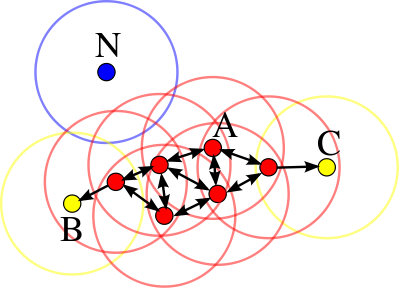
\includegraphics{img/dbscan.png}

Pada gambar diatas, titik yang berwarna merah merupakan
\texttt{core\_point}, titik yang berwarna kuning merupakan
\texttt{border\_point} dan titik yang berwarna biru merupakan
\texttt{noise\_data} atau outlier.

Perhitungan jarak yang dapat digunakan pada implemetasi DBSCAN ini ada
dua macam yaitu jarak euclidean dan jarak manhtattan.

Berikut ini merupakan pseudocode dari DBSCAN:

\begin{verbatim}
DBSCAN(data, eps, min_pts):
    curr_label = 0
    for data_i in data:
        if data_i is core_point and not yet labelled:
            label = curr_label
            cluster(data_i) = label
            neighbour_stack = [neighbour(data_i)]
            while neighbour_stack is not empty:
                neighbour_data_i = neighbour_stack.pop
                if neighbour_data_i not yet labelled:
                    cluster(neighbour_data_i) = label
                    if neighbour_data_i is core point:
                        neighbour_stack,push(neighbour(neighbour_data_i))
           curr_label += 1
\end{verbatim}

    \subsection{Class}\label{class}

    \begin{Verbatim}[commandchars=\\\{\}]
{\color{incolor}In [{\color{incolor}9}]:} \PY{k+kn}{import} \PY{n+nn}{numpy} \PY{k}{as} \PY{n+nn}{np} 
        \PY{k+kn}{import} \PY{n+nn}{math}
        
        \PY{k}{class} \PY{n+nc}{tes\PYZus{}DBSCAN}\PY{p}{:}
            
            \PY{n}{UNLABELLED\PYZus{}DATA} \PY{o}{=} \PY{o}{\PYZhy{}}\PY{l+m+mi}{1}
            
            \PY{n}{n\PYZus{}clusters} \PY{o}{=} \PY{k+kc}{None}
            \PY{n}{result} \PY{o}{=} \PY{k+kc}{None}
                
            \PY{n}{metrics} \PY{o}{=} \PY{l+s+s1}{\PYZsq{}}\PY{l+s+s1}{euclidean}\PY{l+s+s1}{\PYZsq{}}    
            \PY{n}{eps} \PY{o}{=} \PY{l+m+mf}{0.5}
            \PY{n}{min\PYZus{}pts} \PY{o}{=} \PY{l+m+mi}{5}
            \PY{n}{available\PYZus{}metrics} \PY{o}{=} \PY{p}{[}\PY{l+s+s1}{\PYZsq{}}\PY{l+s+s1}{euclidean}\PY{l+s+s1}{\PYZsq{}}\PY{p}{,} \PY{l+s+s1}{\PYZsq{}}\PY{l+s+s1}{manhattan}\PY{l+s+s1}{\PYZsq{}}\PY{p}{]}
        
            \PY{k}{def} \PY{n+nf}{\PYZus{}\PYZus{}init\PYZus{}\PYZus{}} \PY{p}{(}\PY{n+nb+bp}{self}\PY{p}{,} \PY{n}{min\PYZus{}pts}\PY{o}{=}\PY{n}{min\PYZus{}pts}\PY{p}{,} \PY{n}{eps}\PY{o}{=}\PY{n}{eps}\PY{p}{,} \PY{n}{metrics}\PY{o}{=}\PY{n}{metrics}\PY{p}{)}\PY{p}{:}
                \PY{l+s+sd}{\PYZsq{}\PYZsq{}\PYZsq{}}
        \PY{l+s+sd}{        Inisiasi kelas dengan min\PYZus{}pts dan epsilon}
        \PY{l+s+sd}{        \PYZsq{}\PYZsq{}\PYZsq{}}
                \PY{k}{if} \PY{n}{eps} \PY{o}{\PYZlt{}}\PY{o}{=} \PY{l+m+mi}{0}\PY{p}{:}
                    \PY{k}{raise} \PY{n+ne}{Exception}\PY{p}{(}\PY{l+s+s1}{\PYZsq{}}\PY{l+s+s1}{eps must be higher than 0}\PY{l+s+s1}{\PYZsq{}}\PY{p}{)}
                \PY{k}{if} \PY{n}{min\PYZus{}pts} \PY{o}{\PYZlt{}}\PY{o}{=} \PY{l+m+mi}{0}\PY{p}{:}
                    \PY{k}{raise} \PY{n+ne}{Exception}\PY{p}{(}\PY{l+s+s1}{\PYZsq{}}\PY{l+s+s1}{min\PYZus{}pts must be higher than 0}\PY{l+s+s1}{\PYZsq{}}\PY{p}{)}
                \PY{k}{if} \PY{n}{metrics} \PY{o+ow}{not} \PY{o+ow}{in} \PY{n+nb+bp}{self}\PY{o}{.}\PY{n}{available\PYZus{}metrics}\PY{p}{:}
                    \PY{k}{raise} \PY{n+ne}{Exception}\PY{p}{(}\PY{l+s+s1}{\PYZsq{}}\PY{l+s+s1}{No metrics }\PY{l+s+se}{\PYZbs{}\PYZsq{}}\PY{l+s+s1}{\PYZsq{}} \PY{o}{+} \PY{n+nb}{str}\PY{p}{(}\PY{n}{metrics}\PY{p}{)} \PY{o}{+} \PY{l+s+s1}{\PYZsq{}}\PY{l+s+se}{\PYZbs{}\PYZsq{}}\PY{l+s+s1}{. Available metrics }\PY{l+s+s1}{\PYZsq{}}\PY{o}{+} \PY{n+nb}{str}\PY{p}{(}\PY{n+nb+bp}{self}\PY{o}{.}\PY{n}{available\PYZus{}metrics}\PY{p}{)}\PY{p}{)}
                    
                \PY{n+nb+bp}{self}\PY{o}{.}\PY{n}{min\PYZus{}pts} \PY{o}{=} \PY{n}{min\PYZus{}pts}
                \PY{n+nb+bp}{self}\PY{o}{.}\PY{n}{eps} \PY{o}{=} \PY{n}{eps}
                \PY{n+nb+bp}{self}\PY{o}{.}\PY{n}{metrics}\PY{o}{=}\PY{n}{metrics}
                
            \PY{k}{def} \PY{n+nf}{\PYZus{}\PYZus{}euclidean\PYZus{}distance}\PY{p}{(}\PY{n+nb+bp}{self}\PY{p}{,} \PY{n}{point\PYZus{}a}\PY{p}{,} \PY{n}{point\PYZus{}b}\PY{p}{)}\PY{p}{:}
                \PY{l+s+sd}{\PYZsq{}\PYZsq{}\PYZsq{}}
        \PY{l+s+sd}{        Fungsi untuk menghitung euclidean distance}
        \PY{l+s+sd}{        \PYZsq{}\PYZsq{}\PYZsq{}}
                \PY{n}{dist} \PY{o}{=} \PY{l+m+mi}{0}
                \PY{k}{for} \PY{n}{a}\PY{p}{,} \PY{n}{b} \PY{o+ow}{in} \PY{n+nb}{zip}\PY{p}{(}\PY{n}{point\PYZus{}a}\PY{p}{,} \PY{n}{point\PYZus{}b}\PY{p}{)}\PY{p}{:}
                    \PY{n}{dist} \PY{o}{+}\PY{o}{=} \PY{p}{(}\PY{n}{a} \PY{o}{\PYZhy{}} \PY{n}{b}\PY{p}{)} \PY{o}{*} \PY{p}{(}\PY{n}{a} \PY{o}{\PYZhy{}} \PY{n}{b}\PY{p}{)}
                \PY{k}{return} \PY{n}{np}\PY{o}{.}\PY{n}{sqrt}\PY{p}{(}\PY{n}{dist}\PY{p}{)}
        
            \PY{k}{def} \PY{n+nf}{\PYZus{}\PYZus{}manhattan\PYZus{}distance}\PY{p}{(}\PY{n+nb+bp}{self}\PY{p}{,} \PY{n}{point\PYZus{}a}\PY{p}{,} \PY{n}{point\PYZus{}b}\PY{p}{)}\PY{p}{:}
                \PY{l+s+sd}{\PYZsq{}\PYZsq{}\PYZsq{}}
        \PY{l+s+sd}{        Fungsi untuk menghitung manhattan distance }
        \PY{l+s+sd}{        \PYZsq{}\PYZsq{}\PYZsq{}}
                \PY{n}{dist} \PY{o}{=} \PY{l+m+mi}{0}
                \PY{k}{for} \PY{n}{a}\PY{p}{,} \PY{n}{b} \PY{o+ow}{in} \PY{n+nb}{zip}\PY{p}{(}\PY{n}{point\PYZus{}a}\PY{p}{,} \PY{n}{point\PYZus{}b}\PY{p}{)}\PY{p}{:}
                    \PY{n}{dist} \PY{o}{+}\PY{o}{=} \PY{n+nb}{abs}\PY{p}{(}\PY{n}{a} \PY{o}{\PYZhy{}} \PY{n}{b}\PY{p}{)}
                \PY{k}{return} \PY{n}{dist}
            
            \PY{k}{def} \PY{n+nf}{\PYZus{}\PYZus{}distance}\PY{p}{(}\PY{n+nb+bp}{self}\PY{p}{,} \PY{n}{point\PYZus{}a}\PY{p}{,} \PY{n}{point\PYZus{}b}\PY{p}{,} \PY{n}{metrics}\PY{o}{=}\PY{n}{metrics}\PY{p}{)}\PY{p}{:}
                \PY{l+s+sd}{\PYZsq{}\PYZsq{}\PYZsq{}}
        \PY{l+s+sd}{        Fungsi untuk mencari jarak berdasarkan metricsnya}
        \PY{l+s+sd}{        \PYZsq{}\PYZsq{}\PYZsq{}}
                \PY{k}{if} \PY{n+nb}{len}\PY{p}{(}\PY{n}{point\PYZus{}a}\PY{p}{)} \PY{o}{==} \PY{n+nb}{len}\PY{p}{(}\PY{n}{point\PYZus{}b}\PY{p}{)}\PY{p}{:}
                    \PY{k}{if} \PY{n}{metrics} \PY{o}{==} \PY{l+s+s1}{\PYZsq{}}\PY{l+s+s1}{euclidean}\PY{l+s+s1}{\PYZsq{}}\PY{p}{:}
                        \PY{k}{return} \PY{n+nb+bp}{self}\PY{o}{.}\PY{n}{\PYZus{}\PYZus{}euclidean\PYZus{}distance}\PY{p}{(}\PY{n}{point\PYZus{}a}\PY{p}{,} \PY{n}{point\PYZus{}b}\PY{p}{)}
                    \PY{k}{if} \PY{n}{metrics} \PY{o}{==} \PY{l+s+s1}{\PYZsq{}}\PY{l+s+s1}{manhattan}\PY{l+s+s1}{\PYZsq{}}\PY{p}{:}
                        \PY{k}{return} \PY{n+nb+bp}{self}\PY{o}{.}\PY{n}{\PYZus{}\PYZus{}manhattan\PYZus{}distance}\PY{p}{(}\PY{n}{point\PYZus{}a}\PY{p}{,} \PY{n}{point\PYZus{}b}\PY{p}{)}
                \PY{k}{else}\PY{p}{:}
                    \PY{k}{raise} \PY{n+ne}{Exception}\PY{p}{(}\PY{l+s+s2}{\PYZdq{}}\PY{l+s+s2}{feature length doesn}\PY{l+s+s2}{\PYZsq{}}\PY{l+s+s2}{t same}\PY{l+s+s2}{\PYZdq{}}\PY{p}{)}
            
            \PY{k}{def} \PY{n+nf}{fit\PYZus{}predict}\PY{p}{(}\PY{n+nb+bp}{self}\PY{p}{,} \PY{n}{data}\PY{p}{)}\PY{p}{:}
                \PY{l+s+sd}{\PYZsq{}\PYZsq{}\PYZsq{}}
        \PY{l+s+sd}{        Fungsi untuk mengelompolkkan data}
        \PY{l+s+sd}{        \PYZsq{}\PYZsq{}\PYZsq{}}
                \PY{n}{size\PYZus{}data} \PY{o}{=} \PY{n+nb}{len}\PY{p}{(}\PY{n}{data}\PY{p}{)}
                
                \PY{c+c1}{\PYZsh{} generate all neighbours }
                \PY{n}{neighbours} \PY{o}{=} \PY{p}{[}\PY{p}{]}
                \PY{k}{for} \PY{n}{i} \PY{o+ow}{in} \PY{n+nb}{range}\PY{p}{(}\PY{n}{size\PYZus{}data}\PY{p}{)}\PY{p}{:}
                    \PY{n}{neighbour\PYZus{}i} \PY{o}{=} \PY{p}{[}\PY{p}{]}
                    \PY{k}{for} \PY{n}{j} \PY{o+ow}{in} \PY{n+nb}{range}\PY{p}{(}\PY{n}{size\PYZus{}data}\PY{p}{)}\PY{p}{:}
                        \PY{k}{if} \PY{n+nb+bp}{self}\PY{o}{.}\PY{n}{\PYZus{}\PYZus{}distance}\PY{p}{(}\PY{n}{data}\PY{p}{[}\PY{n}{i}\PY{p}{]}\PY{p}{,} \PY{n}{data}\PY{p}{[}\PY{n}{j}\PY{p}{]}\PY{p}{,} \PY{n+nb+bp}{self}\PY{o}{.}\PY{n}{metrics}\PY{p}{)} \PY{o}{\PYZlt{}}\PY{o}{=} \PY{n+nb+bp}{self}\PY{o}{.}\PY{n}{eps}\PY{p}{:}
                            \PY{n}{neighbour\PYZus{}i}\PY{o}{.}\PY{n}{append}\PY{p}{(}\PY{n}{j}\PY{p}{)}
                    \PY{n}{neighbours}\PY{o}{.}\PY{n}{append}\PY{p}{(}\PY{n}{neighbour\PYZus{}i}\PY{p}{)}
                
                \PY{c+c1}{\PYZsh{} initialize label}
                \PY{n+nb+bp}{self}\PY{o}{.}\PY{n}{result} \PY{o}{=} \PY{n}{np}\PY{o}{.}\PY{n}{full}\PY{p}{(}\PY{p}{(}\PY{n}{size\PYZus{}data}\PY{p}{)}\PY{p}{,} \PY{n+nb+bp}{self}\PY{o}{.}\PY{n}{UNLABELLED\PYZus{}DATA}\PY{p}{)}
                
                \PY{c+c1}{\PYZsh{} giving label to data}
                \PY{n}{curr\PYZus{}label} \PY{o}{=} \PY{l+m+mi}{0}
                \PY{k}{for} \PY{n}{i} \PY{o+ow}{in} \PY{n+nb}{range}\PY{p}{(}\PY{n}{size\PYZus{}data}\PY{p}{)}\PY{p}{:}
                    \PY{c+c1}{\PYZsh{} if neighbours \PYZgt{} min\PYZus{}pts (data\PYZus{}i is core points) and not yet labelled, then give label }
                    \PY{k}{if} \PY{n+nb}{len}\PY{p}{(}\PY{n}{neighbours}\PY{p}{[}\PY{n}{i}\PY{p}{]}\PY{p}{)} \PY{o}{\PYZgt{}}\PY{o}{=} \PY{n+nb+bp}{self}\PY{o}{.}\PY{n}{min\PYZus{}pts} \PY{o+ow}{and} \PY{n+nb+bp}{self}\PY{o}{.}\PY{n}{result}\PY{p}{[}\PY{n}{i}\PY{p}{]} \PY{o}{==} \PY{n+nb+bp}{self}\PY{o}{.}\PY{n}{UNLABELLED\PYZus{}DATA}\PY{p}{:} 
                        \PY{n}{label} \PY{o}{=} \PY{n}{curr\PYZus{}label}
                        \PY{c+c1}{\PYZsh{} giving label to all neighbours}
                        \PY{n}{neighbours\PYZus{}i} \PY{o}{=} \PY{p}{[}\PY{n}{i}\PY{p}{]}
                        \PY{k}{while} \PY{n+nb}{len}\PY{p}{(}\PY{n}{neighbours\PYZus{}i}\PY{p}{)} \PY{o}{\PYZgt{}} \PY{l+m+mi}{0}\PY{p}{:}
                            \PY{n}{neigh\PYZus{}i} \PY{o}{=} \PY{n}{neighbours\PYZus{}i}\PY{o}{.}\PY{n}{pop}\PY{p}{(}\PY{p}{)}
                            \PY{c+c1}{\PYZsh{} if not yet labelled then give label to data and the neighbours}
                            \PY{k}{if} \PY{n+nb+bp}{self}\PY{o}{.}\PY{n}{result}\PY{p}{[}\PY{n}{neigh\PYZus{}i}\PY{p}{]} \PY{o}{==} \PY{n+nb+bp}{self}\PY{o}{.}\PY{n}{UNLABELLED\PYZus{}DATA}\PY{p}{:}
                                \PY{n+nb+bp}{self}\PY{o}{.}\PY{n}{result}\PY{p}{[}\PY{n}{neigh\PYZus{}i}\PY{p}{]} \PY{o}{=} \PY{n}{label}
                                \PY{c+c1}{\PYZsh{} if neigh\PYZus{}i is core point, then give label to the neighbour}
                                \PY{k}{if} \PY{n+nb}{len}\PY{p}{(}\PY{n}{neighbours}\PY{p}{[}\PY{n}{neigh\PYZus{}i}\PY{p}{]}\PY{p}{)} \PY{o}{\PYZgt{}}\PY{o}{=} \PY{n+nb+bp}{self}\PY{o}{.}\PY{n}{min\PYZus{}pts}\PY{p}{:}
                                    \PY{n}{neighbours\PYZus{}i} \PY{o}{+}\PY{o}{=} \PY{n}{neighbours}\PY{p}{[}\PY{n}{neigh\PYZus{}i}\PY{p}{]}
                        \PY{n}{curr\PYZus{}label} \PY{o}{+}\PY{o}{=} \PY{l+m+mi}{1}
                
                \PY{n+nb+bp}{self}\PY{o}{.}\PY{n}{n\PYZus{}clusters} \PY{o}{=} \PY{n}{curr\PYZus{}label}           
                \PY{k}{return} \PY{n+nb+bp}{self}\PY{o}{.}\PY{n}{result}
            
            \PY{k}{def} \PY{n+nf}{get\PYZus{}n\PYZus{}clusters}\PY{p}{(}\PY{n+nb+bp}{self}\PY{p}{)}\PY{p}{:}
                \PY{k}{if} \PY{n+nb+bp}{self}\PY{o}{.}\PY{n}{n\PYZus{}clusters} \PY{o+ow}{is} \PY{k+kc}{None}\PY{p}{:}
                    \PY{n+nb}{print}\PY{p}{(}\PY{l+s+s2}{\PYZdq{}}\PY{l+s+s2}{No data}\PY{l+s+s2}{\PYZdq{}}\PY{p}{)}
                \PY{k}{else}\PY{p}{:}
                    \PY{k}{return} \PY{n+nb+bp}{self}\PY{o}{.}\PY{n}{n\PYZus{}clusters}
            
            \PY{k}{def} \PY{n+nf}{get\PYZus{}epsilon}\PY{p}{(}\PY{n+nb+bp}{self}\PY{p}{)}\PY{p}{:}
                \PY{k}{return} \PY{n+nb+bp}{self}\PY{o}{.}\PY{n}{eps}
        
            \PY{k}{def} \PY{n+nf}{get\PYZus{}metrics}\PY{p}{(}\PY{n+nb+bp}{self}\PY{p}{)}\PY{p}{:}
                \PY{k}{return} \PY{n+nb+bp}{self}\PY{o}{.}\PY{n}{metrics}
            
            \PY{k}{def} \PY{n+nf}{get\PYZus{}min\PYZus{}pts}\PY{p}{(}\PY{n+nb+bp}{self}\PY{p}{)}\PY{p}{:}
                \PY{k}{return} \PY{n+nb+bp}{self}\PY{o}{.}\PY{n}{min\PYZus{}pts}
            
\end{Verbatim}


    \subsection{Experiments}\label{experiments}

Berikut ini merupakan hasil eksperimen implementasi DBSCAN untuk
clustering data iris menggunakan \emph{euclidean disntance}.

    \begin{Verbatim}[commandchars=\\\{\}]
{\color{incolor}In [{\color{incolor}10}]:} \PY{k+kn}{from} \PY{n+nn}{sklearn} \PY{k}{import} \PY{n}{datasets}
         
         \PY{n}{iris} \PY{o}{=} \PY{n}{datasets}\PY{o}{.}\PY{n}{load\PYZus{}iris}\PY{p}{(}\PY{p}{)}
         \PY{n}{data} \PY{o}{=} \PY{n}{iris}\PY{o}{.}\PY{n}{data}
         \PY{n}{label} \PY{o}{=} \PY{n}{iris}\PY{o}{.}\PY{n}{target}
\end{Verbatim}


    \begin{Verbatim}[commandchars=\\\{\}]
{\color{incolor}In [{\color{incolor}11}]:} \PY{k+kn}{import} \PY{n+nn}{time}
         
         \PY{n}{dbscan} \PY{o}{=} \PY{n}{tes\PYZus{}DBSCAN}\PY{p}{(}\PY{n}{eps}\PY{o}{=}\PY{l+m+mf}{0.5}\PY{p}{,} \PY{n}{min\PYZus{}pts}\PY{o}{=}\PY{l+m+mi}{4}\PY{p}{,} \PY{n}{metrics}\PY{o}{=}\PY{l+s+s1}{\PYZsq{}}\PY{l+s+s1}{euclidean}\PY{l+s+s1}{\PYZsq{}}\PY{p}{)}
         
         \PY{n}{start} \PY{o}{=} \PY{n}{time}\PY{o}{.}\PY{n}{time}\PY{p}{(}\PY{p}{)}
         
         \PY{n}{pred} \PY{o}{=} \PY{n}{dbscan}\PY{o}{.}\PY{n}{fit\PYZus{}predict}\PY{p}{(}\PY{n}{data}\PY{p}{)}
         
         \PY{n+nb}{print}\PY{p}{(}\PY{l+s+s2}{\PYZdq{}}\PY{l+s+s2}{\PYZhy{}\PYZhy{}\PYZhy{}\PYZhy{} Time taken: }\PY{l+s+si}{\PYZob{}\PYZcb{}}\PY{l+s+s2}{ s \PYZhy{}\PYZhy{}\PYZhy{}\PYZhy{}}\PY{l+s+s2}{\PYZdq{}}\PY{o}{.}\PY{n}{format}\PY{p}{(}\PY{n}{time}\PY{o}{.}\PY{n}{time}\PY{p}{(}\PY{p}{)} \PY{o}{\PYZhy{}} \PY{n}{start}\PY{p}{)}\PY{p}{)}
         \PY{n+nb}{print}\PY{p}{(}\PY{l+s+s2}{\PYZdq{}}\PY{l+s+s2}{\PYZhy{}\PYZhy{}\PYZhy{}\PYZhy{} Cluster: }\PY{l+s+si}{\PYZob{}\PYZcb{}}\PY{l+s+s2}{ \PYZhy{}\PYZhy{}\PYZhy{}\PYZhy{}}\PY{l+s+s2}{\PYZdq{}}\PY{o}{.}\PY{n}{format}\PY{p}{(}\PY{n}{dbscan}\PY{o}{.}\PY{n}{get\PYZus{}n\PYZus{}clusters}\PY{p}{(}\PY{p}{)}\PY{p}{)}\PY{p}{)}
         \PY{n+nb}{print}\PY{p}{(}\PY{l+s+s2}{\PYZdq{}}\PY{l+s+s2}{Cluster prediction:}\PY{l+s+s2}{\PYZdq{}}\PY{p}{)}
         \PY{n+nb}{print}\PY{p}{(}\PY{n}{pred}\PY{p}{)}
         \PY{n+nb}{print}\PY{p}{(}\PY{l+s+s2}{\PYZdq{}}\PY{l+s+s2}{Purity: }\PY{l+s+si}{\PYZob{}\PYZcb{}}\PY{l+s+s2}{\PYZdq{}}\PY{o}{.}\PY{n}{format}\PY{p}{(}\PY{n}{purity}\PY{p}{(}\PY{n}{pred}\PY{p}{,} \PY{n}{label}\PY{p}{)}\PY{p}{)}\PY{p}{)}
\end{Verbatim}


    \begin{Verbatim}[commandchars=\\\{\}]
---- Time taken: 0.3169534206390381 s ----
---- Cluster: 3 ----
Cluster prediction:
[ 0  0  0  0  0  0  0  0  0  0  0  0  0  0  0  0  0  0  0  0  0  0  0  0
  0  0  0  0  0  0  0  0  0  0  0  0  0  0  0  0  0 -1  0  0  0  0  0  0
  0  0  1  1  1  1  1  1  1  2  1  1  2  1  1  1  1  1  1  1 -1  1  1  1
  1  1  1  1  1  1  1  1  1  1  1  1  1  1  1 -1  1  1  1  1  1  2  1  1
  1  1  2  1  1  1  1  1  1 -1 -1  1 -1 -1  1  1  1  1  1  1  1 -1 -1  1
  1  1 -1  1  1  1  1  1  1  1  1 -1  1  1 -1 -1  1  1  1  1  1  1  1  1
  1  1  1  1  1  1]
Purity: 0.708029197080292

    \end{Verbatim}

    \begin{Verbatim}[commandchars=\\\{\}]
{\color{incolor}In [{\color{incolor}12}]:} \PY{n}{dbscan} \PY{o}{=} \PY{n}{tes\PYZus{}DBSCAN}\PY{p}{(}\PY{n}{eps}\PY{o}{=}\PY{l+m+mi}{1}\PY{p}{,} \PY{n}{min\PYZus{}pts}\PY{o}{=}\PY{l+m+mi}{3}\PY{p}{,} \PY{n}{metrics}\PY{o}{=}\PY{l+s+s1}{\PYZsq{}}\PY{l+s+s1}{euclidean}\PY{l+s+s1}{\PYZsq{}}\PY{p}{)}
         
         \PY{n}{start} \PY{o}{=} \PY{n}{time}\PY{o}{.}\PY{n}{time}\PY{p}{(}\PY{p}{)}
         
         \PY{n}{pred} \PY{o}{=} \PY{n}{dbscan}\PY{o}{.}\PY{n}{fit\PYZus{}predict}\PY{p}{(}\PY{n}{data}\PY{p}{)}
         
         \PY{n+nb}{print}\PY{p}{(}\PY{l+s+s2}{\PYZdq{}}\PY{l+s+s2}{\PYZhy{}\PYZhy{}\PYZhy{}\PYZhy{} Time taken: }\PY{l+s+si}{\PYZob{}\PYZcb{}}\PY{l+s+s2}{ s \PYZhy{}\PYZhy{}\PYZhy{}\PYZhy{}}\PY{l+s+s2}{\PYZdq{}}\PY{o}{.}\PY{n}{format}\PY{p}{(}\PY{n}{time}\PY{o}{.}\PY{n}{time}\PY{p}{(}\PY{p}{)} \PY{o}{\PYZhy{}} \PY{n}{start}\PY{p}{)}\PY{p}{)}
         \PY{n+nb}{print}\PY{p}{(}\PY{l+s+s2}{\PYZdq{}}\PY{l+s+s2}{\PYZhy{}\PYZhy{}\PYZhy{}\PYZhy{} Cluster: }\PY{l+s+si}{\PYZob{}\PYZcb{}}\PY{l+s+s2}{ \PYZhy{}\PYZhy{}\PYZhy{}\PYZhy{}}\PY{l+s+s2}{\PYZdq{}}\PY{o}{.}\PY{n}{format}\PY{p}{(}\PY{n}{dbscan}\PY{o}{.}\PY{n}{get\PYZus{}n\PYZus{}clusters}\PY{p}{(}\PY{p}{)}\PY{p}{)}\PY{p}{)}
         \PY{n+nb}{print}\PY{p}{(}\PY{l+s+s2}{\PYZdq{}}\PY{l+s+s2}{Cluster prediction:}\PY{l+s+s2}{\PYZdq{}}\PY{p}{)}
         \PY{n+nb}{print}\PY{p}{(}\PY{n}{pred}\PY{p}{)}
         \PY{n+nb}{print}\PY{p}{(}\PY{l+s+s2}{\PYZdq{}}\PY{l+s+s2}{Purity: }\PY{l+s+si}{\PYZob{}\PYZcb{}}\PY{l+s+s2}{\PYZdq{}}\PY{o}{.}\PY{n}{format}\PY{p}{(}\PY{n}{purity}\PY{p}{(}\PY{n}{pred}\PY{p}{,} \PY{n}{label}\PY{p}{)}\PY{p}{)}\PY{p}{)}
\end{Verbatim}


    \begin{Verbatim}[commandchars=\\\{\}]
---- Time taken: 0.2816331386566162 s ----
---- Cluster: 2 ----
Cluster prediction:
[0 0 0 0 0 0 0 0 0 0 0 0 0 0 0 0 0 0 0 0 0 0 0 0 0 0 0 0 0 0 0 0 0 0 0 0 0
 0 0 0 0 0 0 0 0 0 0 0 0 0 1 1 1 1 1 1 1 1 1 1 1 1 1 1 1 1 1 1 1 1 1 1 1 1
 1 1 1 1 1 1 1 1 1 1 1 1 1 1 1 1 1 1 1 1 1 1 1 1 1 1 1 1 1 1 1 1 1 1 1 1 1
 1 1 1 1 1 1 1 1 1 1 1 1 1 1 1 1 1 1 1 1 1 1 1 1 1 1 1 1 1 1 1 1 1 1 1 1 1
 1 1]
Purity: 0.6666666666666666

    \end{Verbatim}

    \subsection{Hasil Eksperimen}\label{hasil-eksperimen}

Dari kedua hasil eksperimen diatas, dapat dilihat bahwa DBSCAN mampu
mengelompokkan data iris dalam waktu sekitar 0.2 - 0.3 detik. Namun
kedua eksperimen menghasilkan nilai purity yang berbeda, hal ini
dikarenakan perbedaan nilai \texttt{epsilon} dan \texttt{min\_pts}.
Dengan nilai \texttt{epsilon} 0.5 dan \texttt{min\_pts} 4, DBSCAN
menghasilkan 3 kluster dan beberapa data yang dianggap outlier.
Sedangkan dengan nilai \texttt{epsilon} 1 dan \texttt{min\_pts} 3,
DBSCAN menghasilkan 2 kluster dan tanpa ada data yang dianggap outlier.
Hal ini menunjukkan bahwa DBSCAN akan sangat bergantung terhadap kedua
nilai tersebut dan ini merupakan tantangan dalam menggunakan DBSCAN.

    \subsection{\# KMeans}\label{kmeans}

\emph{KMeans} merupakan suatu teknik dalam melakukan \emph{clustering}
yang menggunakan pendekatan \emph{partitioning}. Ide utama dari teknik
ini adalah dengan mengelompokkan data ke K \emph{cluster}. Penentuan
\emph{cluster} mana untuk data tertentu yaitu dengan cara menghitung
jarak data tersebut dengan representasi dari \emph{cluster}
(\emph{centroid}). Representasi dari \emph{cluster} berupa rata-rata
(\emph{means}) dari data-data anggota \emph{cluster} tersebut.
Penghitungan jarak dengan menggunakan \emph{euclidean distance}.

\begin{figure}[htbp]
\centering
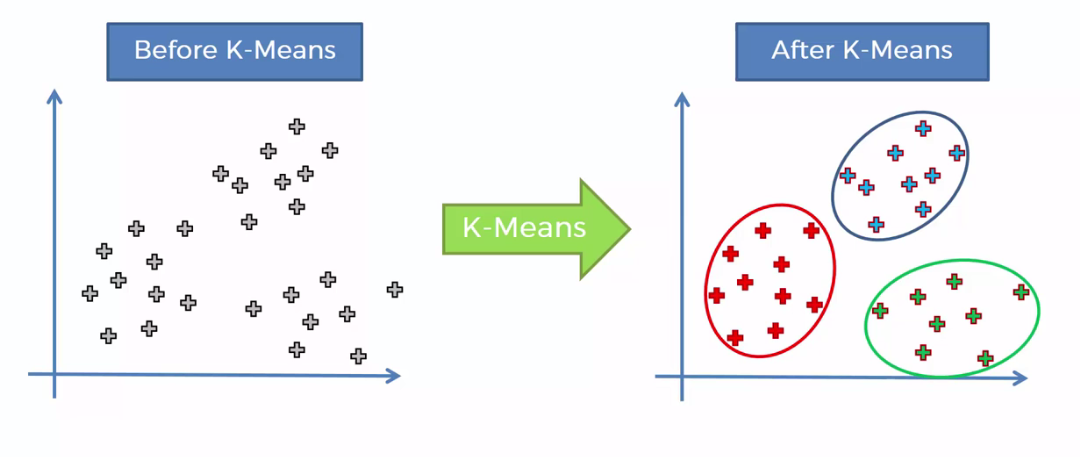
\includegraphics{img/kmeans.png}
\caption{kmeans}
\end{figure}

Dalam notasi \emph{pseudocode}, algoritma \emph{KMeans} adalah sebagai
berikut.

\begin{verbatim}
choose_initial_centroid()
WHILE (any_change_in_cluster) DO
    FOREACH object
        assign_to_cluster(object)
    FOREACH cluster
        update_cluster_means(cluster)
\end{verbatim}

    \subsection{Implementation Class}\label{implementation-class}

    \begin{Verbatim}[commandchars=\\\{\}]
{\color{incolor}In [{\color{incolor}13}]:} \PY{k+kn}{import} \PY{n+nn}{numpy} \PY{k}{as} \PY{n+nn}{np}
         \PY{k+kn}{import} \PY{n+nn}{math}
         \PY{k+kn}{import} \PY{n+nn}{random}
         
         \PY{k}{class} \PY{n+nc}{KMeans}\PY{p}{:}
             \PY{l+s+sd}{\PYZsq{}\PYZsq{}\PYZsq{}}
         \PY{l+s+sd}{    Kelas untuk mengakomodasi nilai metode KMeans clustering}
         \PY{l+s+sd}{    \PYZsq{}\PYZsq{}\PYZsq{}}
             \PY{c+c1}{\PYZsh{} Nilai default parameter}
             \PY{n}{n\PYZus{}clusters} \PY{o}{=} \PY{l+m+mi}{2}
             \PY{n}{init} \PY{o}{=} \PY{l+s+s1}{\PYZsq{}}\PY{l+s+s1}{random}\PY{l+s+s1}{\PYZsq{}}
             \PY{n}{max\PYZus{}iter} \PY{o}{=} \PY{l+m+mi}{300}
             \PY{n}{init\PYZus{}val} \PY{o}{=} \PY{p}{[}\PY{p}{]}
             
             \PY{n}{available\PYZus{}init} \PY{o}{=} \PY{p}{[}\PY{l+s+s1}{\PYZsq{}}\PY{l+s+s1}{random}\PY{l+s+s1}{\PYZsq{}}\PY{p}{,} \PY{l+s+s1}{\PYZsq{}}\PY{l+s+s1}{manual}\PY{l+s+s1}{\PYZsq{}}\PY{p}{]}
             
             \PY{k}{def} \PY{n+nf}{\PYZus{}\PYZus{}init\PYZus{}\PYZus{}}\PY{p}{(}\PY{n+nb+bp}{self}\PY{p}{,} \PY{n}{n\PYZus{}clusters}\PY{o}{=}\PY{n}{n\PYZus{}clusters}\PY{p}{,} \PY{n}{init}\PY{o}{=}\PY{n}{init}\PY{p}{,} \PY{n}{init\PYZus{}val}\PY{o}{=}\PY{n}{init\PYZus{}val}\PY{p}{,} \PY{n}{max\PYZus{}iter}\PY{o}{=}\PY{n}{max\PYZus{}iter}\PY{p}{)}\PY{p}{:}
                 \PY{l+s+sd}{\PYZsq{}\PYZsq{}\PYZsq{}}
         \PY{l+s+sd}{        Inisiasi kelas. Parameter yang dibutuhkan untuk setiap kelas diinisiasi atau diisi dengan nilai default }
         \PY{l+s+sd}{        \PYZsq{}\PYZsq{}\PYZsq{}}    
                 \PY{k}{if} \PY{n}{n\PYZus{}clusters} \PY{o}{\PYZlt{}}\PY{o}{=} \PY{l+m+mi}{0}\PY{p}{:}
                     \PY{k}{raise} \PY{n+ne}{Exception}\PY{p}{(}\PY{l+s+s1}{\PYZsq{}}\PY{l+s+s1}{n\PYZus{}clusters must be higher than 0}\PY{l+s+s1}{\PYZsq{}}\PY{p}{)}
                 \PY{k}{if} \PY{n}{init} \PY{o+ow}{not} \PY{o+ow}{in} \PY{n+nb+bp}{self}\PY{o}{.}\PY{n}{available\PYZus{}init}\PY{p}{:}
                     \PY{k}{raise} \PY{n+ne}{Exception}\PY{p}{(}\PY{l+s+s1}{\PYZsq{}}\PY{l+s+s1}{No init method }\PY{l+s+se}{\PYZbs{}\PYZsq{}}\PY{l+s+s1}{\PYZsq{}} \PY{o}{+} \PY{n+nb}{str}\PY{p}{(}\PY{n}{init}\PY{p}{)} \PY{o}{+} \PY{l+s+s1}{\PYZsq{}}\PY{l+s+se}{\PYZbs{}\PYZsq{}}\PY{l+s+s1}{. Available init methods}\PY{l+s+s1}{\PYZsq{}}\PY{o}{+} \PY{n+nb}{str}\PY{p}{(}\PY{n+nb+bp}{self}\PY{o}{.}\PY{n}{available\PYZus{}init}\PY{p}{)}\PY{p}{)}
                 \PY{k}{if} \PY{p}{(}\PY{n}{init} \PY{o}{==} \PY{l+s+s1}{\PYZsq{}}\PY{l+s+s1}{manual}\PY{l+s+s1}{\PYZsq{}} \PY{o+ow}{and} \PY{n+nb}{len}\PY{p}{(}\PY{n}{init\PYZus{}val}\PY{p}{)} \PY{o}{!=} \PY{n}{n\PYZus{}clusters}\PY{p}{)}\PY{p}{:}
                     \PY{k}{raise} \PY{n+ne}{Exception}\PY{p}{(}\PY{l+s+s1}{\PYZsq{}}\PY{l+s+s1}{init\PYZus{}val length doesn}\PY{l+s+se}{\PYZbs{}\PYZsq{}}\PY{l+s+s1}{t match with n\PYZus{}clusters }\PY{l+s+s1}{\PYZsq{}}\PY{o}{+} \PY{n+nb}{str}\PY{p}{(}\PY{n}{n\PYZus{}clusters}\PY{p}{)}\PY{p}{)}
                 \PY{n+nb+bp}{self}\PY{o}{.}\PY{n}{n\PYZus{}clusters} \PY{o}{=} \PY{n}{n\PYZus{}clusters}
                 \PY{n+nb+bp}{self}\PY{o}{.}\PY{n}{init} \PY{o}{=} \PY{n}{init}
                 \PY{n+nb+bp}{self}\PY{o}{.}\PY{n}{max\PYZus{}iter} \PY{o}{=} \PY{n}{max\PYZus{}iter}
                 \PY{n+nb+bp}{self}\PY{o}{.}\PY{n}{init\PYZus{}val} \PY{o}{=} \PY{n}{init\PYZus{}val}
             
             \PY{k}{def} \PY{n+nf}{\PYZus{}\PYZus{}is\PYZus{}in\PYZus{}array}\PY{p}{(}\PY{n+nb+bp}{self}\PY{p}{,} \PY{n}{data}\PY{p}{,} \PY{n}{arr}\PY{p}{)}\PY{p}{:}
                 \PY{l+s+sd}{\PYZsq{}\PYZsq{}\PYZsq{}}
         \PY{l+s+sd}{        Fungsi helper untuk menegecek apakah data berupa array berada pada arr berupa array of array}
         \PY{l+s+sd}{        \PYZsq{}\PYZsq{}\PYZsq{}}
                 \PY{n}{is\PYZus{}exist} \PY{o}{=} \PY{k+kc}{False}
                 \PY{n}{arr\PYZus{}idx} \PY{o}{=} \PY{l+m+mi}{0}
                 \PY{k}{while} \PY{p}{(}\PY{o+ow}{not} \PY{n}{is\PYZus{}exist} \PY{o+ow}{and} \PY{n}{arr\PYZus{}idx} \PY{o}{\PYZlt{}} \PY{n+nb}{len}\PY{p}{(}\PY{n}{arr}\PY{p}{)}\PY{p}{)}\PY{p}{:}
                     \PY{n}{is\PYZus{}data\PYZus{}equal} \PY{o}{=} \PY{k+kc}{True}
                     \PY{n}{data\PYZus{}idx} \PY{o}{=} \PY{l+m+mi}{0}
                     \PY{k}{while} \PY{p}{(}\PY{n}{is\PYZus{}data\PYZus{}equal} \PY{o+ow}{and} \PY{n}{data\PYZus{}idx} \PY{o}{\PYZlt{}} \PY{n+nb}{len}\PY{p}{(}\PY{n}{data}\PY{p}{)}\PY{p}{)}\PY{p}{:}
                         \PY{k}{if} \PY{p}{(}\PY{n}{data}\PY{p}{[}\PY{n}{data\PYZus{}idx}\PY{p}{]} \PY{o}{!=} \PY{n}{arr}\PY{p}{[}\PY{n}{arr\PYZus{}idx}\PY{p}{]}\PY{p}{[}\PY{n}{data\PYZus{}idx}\PY{p}{]}\PY{p}{)}\PY{p}{:}
                             \PY{n}{is\PYZus{}data\PYZus{}equal} \PY{o}{=} \PY{k+kc}{False}
                         \PY{k}{else}\PY{p}{:}
                             \PY{n}{data\PYZus{}idx} \PY{o}{+}\PY{o}{=} \PY{l+m+mi}{1}
                     \PY{k}{if} \PY{n}{is\PYZus{}data\PYZus{}equal}\PY{p}{:}
                         \PY{n}{is\PYZus{}exist} \PY{o}{=} \PY{k+kc}{True}
                     \PY{k}{else}\PY{p}{:}
                         \PY{n}{arr\PYZus{}idx} \PY{o}{+}\PY{o}{=} \PY{l+m+mi}{1}
                 \PY{k}{return} \PY{n}{is\PYZus{}exist}
                 
             \PY{k}{def} \PY{n+nf}{\PYZus{}\PYZus{}euclidean\PYZus{}distance}\PY{p}{(}\PY{n+nb+bp}{self}\PY{p}{,} \PY{n}{data1}\PY{p}{,} \PY{n}{data2}\PY{p}{)}\PY{p}{:}
                 \PY{l+s+sd}{\PYZsq{}\PYZsq{}\PYZsq{}}
         \PY{l+s+sd}{        Fungsi untuk menghitung euclidean distance di antara dua vector dengan panjang yang sama}
         \PY{l+s+sd}{        \PYZsq{}\PYZsq{}\PYZsq{}}
                 \PY{n+nb}{sum} \PY{o}{=} \PY{l+m+mi}{0}
                 \PY{k}{if} \PY{p}{(}\PY{n+nb}{len}\PY{p}{(}\PY{n}{data1}\PY{p}{)} \PY{o}{==} \PY{n+nb}{len}\PY{p}{(}\PY{n}{data2}\PY{p}{)}\PY{p}{)}\PY{p}{:}
                     \PY{k}{for} \PY{n}{x1}\PY{p}{,} \PY{n}{x2} \PY{o+ow}{in} \PY{n+nb}{zip}\PY{p}{(}\PY{n}{data1}\PY{p}{,} \PY{n}{data2}\PY{p}{)}\PY{p}{:}
                         \PY{n+nb}{sum} \PY{o}{+}\PY{o}{=} \PY{p}{(}\PY{n}{x1} \PY{o}{\PYZhy{}} \PY{n}{x2}\PY{p}{)}\PY{o}{*}\PY{o}{*}\PY{l+m+mi}{2}
                     \PY{n}{dist} \PY{o}{=} \PY{n}{math}\PY{o}{.}\PY{n}{sqrt}\PY{p}{(}\PY{n+nb}{sum}\PY{p}{)}
                     \PY{k}{return} \PY{n}{dist}
                 \PY{k}{else}\PY{p}{:}
                     \PY{k}{raise} \PY{n+ne}{Exception}\PY{p}{(}\PY{l+s+s1}{\PYZsq{}}\PY{l+s+s1}{Length doesn}\PY{l+s+se}{\PYZbs{}\PYZsq{}}\PY{l+s+s1}{t match}\PY{l+s+s1}{\PYZsq{}}\PY{p}{)}
                     
             \PY{k}{def} \PY{n+nf}{\PYZus{}\PYZus{}get\PYZus{}distance}\PY{p}{(}\PY{n+nb+bp}{self}\PY{p}{,} \PY{n}{data1}\PY{p}{,} \PY{n}{data2}\PY{p}{)}\PY{p}{:}
                 \PY{l+s+sd}{\PYZsq{}\PYZsq{}\PYZsq{}}
         \PY{l+s+sd}{        Fungsi untuk menghitung jarak dua vector}
         \PY{l+s+sd}{        \PYZsq{}\PYZsq{}\PYZsq{}}
                 \PY{k}{return} \PY{n+nb+bp}{self}\PY{o}{.}\PY{n}{\PYZus{}\PYZus{}euclidean\PYZus{}distance}\PY{p}{(}\PY{n}{data1}\PY{p}{,} \PY{n}{data2}\PY{p}{)}
                 
             \PY{k}{def} \PY{n+nf}{\PYZus{}\PYZus{}calculate\PYZus{}distance\PYZus{}matrix}\PY{p}{(}\PY{n+nb+bp}{self}\PY{p}{,} \PY{n}{data}\PY{p}{,} \PY{n}{centroids}\PY{p}{)}\PY{p}{:}
                 \PY{l+s+sd}{\PYZsq{}\PYZsq{}\PYZsq{}}
         \PY{l+s+sd}{        Fungsi untuk menghitung distance matrix untuk semua data dengan centroid}
         \PY{l+s+sd}{        \PYZsq{}\PYZsq{}\PYZsq{}}
                 \PY{n}{dist\PYZus{}matrix} \PY{o}{=} \PY{p}{[}\PY{p}{]}        
                 \PY{k}{for} \PY{n}{i} \PY{o+ow}{in} \PY{n+nb}{range}\PY{p}{(}\PY{n+nb}{len}\PY{p}{(}\PY{n}{centroids}\PY{p}{)}\PY{p}{)}\PY{p}{:}
                     \PY{n}{dist\PYZus{}curr\PYZus{}centroid} \PY{o}{=} \PY{p}{[}\PY{p}{]}
                     \PY{k}{for} \PY{n}{j} \PY{o+ow}{in} \PY{n+nb}{range}\PY{p}{(}\PY{n+nb}{len}\PY{p}{(}\PY{n}{data}\PY{p}{)}\PY{p}{)}\PY{p}{:}
                         \PY{n}{dist} \PY{o}{=} \PY{n+nb+bp}{self}\PY{o}{.}\PY{n}{\PYZus{}\PYZus{}get\PYZus{}distance}\PY{p}{(}\PY{n}{centroids}\PY{p}{[}\PY{n}{i}\PY{p}{]}\PY{p}{,} \PY{n}{data}\PY{p}{[}\PY{n}{j}\PY{p}{]}\PY{p}{)}
                         \PY{n}{dist\PYZus{}curr\PYZus{}centroid}\PY{o}{.}\PY{n}{append}\PY{p}{(}\PY{n}{dist}\PY{p}{)}
                     \PY{n}{dist\PYZus{}matrix}\PY{o}{.}\PY{n}{append}\PY{p}{(}\PY{n}{dist\PYZus{}curr\PYZus{}centroid}\PY{p}{)}
                 
                 \PY{k}{return} \PY{n}{dist\PYZus{}matrix}
             
             \PY{k}{def} \PY{n+nf}{\PYZus{}\PYZus{}assign\PYZus{}data\PYZus{}to\PYZus{}cluster}\PY{p}{(}\PY{n+nb+bp}{self}\PY{p}{,} \PY{n}{dist\PYZus{}matrix}\PY{p}{)}\PY{p}{:}
                 \PY{l+s+sd}{\PYZsq{}\PYZsq{}\PYZsq{}}
         \PY{l+s+sd}{        Fungsi untuk mengelompokan data berdasarkan jarak yang diketahui}
         \PY{l+s+sd}{        \PYZsq{}\PYZsq{}\PYZsq{}}
                 \PY{n}{cluster\PYZus{}of\PYZus{}data} \PY{o}{=} \PY{p}{[}\PY{p}{]}
                 \PY{k}{for} \PY{n}{j} \PY{o+ow}{in} \PY{n+nb}{range}\PY{p}{(}\PY{n+nb}{len}\PY{p}{(}\PY{n}{dist\PYZus{}matrix}\PY{p}{[}\PY{l+m+mi}{0}\PY{p}{]}\PY{p}{)}\PY{p}{)}\PY{p}{:}
                     \PY{n}{cluster} \PY{o}{=} \PY{l+m+mi}{0}
                     \PY{n}{min\PYZus{}distance} \PY{o}{=} \PY{n}{dist\PYZus{}matrix}\PY{p}{[}\PY{l+m+mi}{0}\PY{p}{]}\PY{p}{[}\PY{n}{j}\PY{p}{]}
                     \PY{k}{for} \PY{n}{i} \PY{o+ow}{in} \PY{n+nb}{range}\PY{p}{(}\PY{l+m+mi}{1}\PY{p}{,}\PY{n+nb}{len}\PY{p}{(}\PY{n}{dist\PYZus{}matrix}\PY{p}{)}\PY{p}{)}\PY{p}{:}
                         \PY{k}{if} \PY{p}{(}\PY{n}{dist\PYZus{}matrix}\PY{p}{[}\PY{n}{i}\PY{p}{]}\PY{p}{[}\PY{n}{j}\PY{p}{]} \PY{o}{\PYZlt{}} \PY{n}{min\PYZus{}distance}\PY{p}{)}\PY{p}{:}
                             \PY{n}{cluster} \PY{o}{=} \PY{n}{i}
                             \PY{n}{min\PYZus{}distance} \PY{o}{=} \PY{n}{dist\PYZus{}matrix}\PY{p}{[}\PY{n}{i}\PY{p}{]}\PY{p}{[}\PY{n}{j}\PY{p}{]}
                     \PY{n}{cluster\PYZus{}of\PYZus{}data}\PY{o}{.}\PY{n}{append}\PY{p}{(}\PY{n}{cluster}\PY{p}{)}
                 \PY{k}{return} \PY{n}{cluster\PYZus{}of\PYZus{}data}
                 
             \PY{k}{def} \PY{n+nf}{\PYZus{}\PYZus{}get\PYZus{}centroids}\PY{p}{(}\PY{n+nb+bp}{self}\PY{p}{,} \PY{n}{data}\PY{p}{,} \PY{n}{cluster\PYZus{}of\PYZus{}data}\PY{p}{)}\PY{p}{:}
                 \PY{l+s+sd}{\PYZsq{}\PYZsq{}\PYZsq{}}
         \PY{l+s+sd}{        Fungsi untuk menghitung centroid baru}
         \PY{l+s+sd}{        \PYZsq{}\PYZsq{}\PYZsq{}}
                 \PY{n}{centroids} \PY{o}{=} \PY{p}{[}\PY{p}{]}
                 \PY{n}{data\PYZus{}per\PYZus{}cluster} \PY{o}{=} \PY{p}{[}\PY{p}{]}
                 \PY{c+c1}{\PYZsh{} inisiasi}
                 \PY{k}{for} \PY{n}{n} \PY{o+ow}{in} \PY{n+nb}{range}\PY{p}{(}\PY{n+nb+bp}{self}\PY{o}{.}\PY{n}{n\PYZus{}clusters}\PY{p}{)}\PY{p}{:}
                     \PY{n}{data\PYZus{}per\PYZus{}cluster}\PY{o}{.}\PY{n}{append}\PY{p}{(}\PY{p}{[}\PY{p}{]}\PY{p}{)}
                 \PY{c+c1}{\PYZsh{} masukkan data ke array tiap cluster}
                 \PY{k}{for} \PY{n}{idx}\PY{p}{,} \PY{n}{data\PYZus{}cluster} \PY{o+ow}{in} \PY{n+nb}{enumerate}\PY{p}{(}\PY{n}{cluster\PYZus{}of\PYZus{}data}\PY{p}{)}\PY{p}{:}
                     \PY{n}{data\PYZus{}per\PYZus{}cluster}\PY{p}{[}\PY{n}{data\PYZus{}cluster}\PY{p}{]}\PY{o}{.}\PY{n}{append}\PY{p}{(}\PY{n}{data}\PY{p}{[}\PY{n}{idx}\PY{p}{]}\PY{p}{)}
                 \PY{c+c1}{\PYZsh{} hitung means}
                 \PY{k}{for} \PY{n}{n} \PY{o+ow}{in} \PY{n+nb}{range}\PY{p}{(}\PY{n+nb+bp}{self}\PY{o}{.}\PY{n}{n\PYZus{}clusters}\PY{p}{)}\PY{p}{:}
                     \PY{k}{if} \PY{n+nb}{len}\PY{p}{(}\PY{n}{data\PYZus{}per\PYZus{}cluster}\PY{p}{[}\PY{n}{n}\PY{p}{]}\PY{p}{)} \PY{o}{\PYZgt{}} \PY{l+m+mi}{0}\PY{p}{:}
                         \PY{n}{means\PYZus{}cluster} \PY{o}{=} \PY{p}{[}\PY{p}{]}
                         \PY{k}{for} \PY{n}{column} \PY{o+ow}{in} \PY{n+nb}{range}\PY{p}{(}\PY{n+nb}{len}\PY{p}{(}\PY{n}{data\PYZus{}per\PYZus{}cluster}\PY{p}{[}\PY{n}{n}\PY{p}{]}\PY{p}{[}\PY{l+m+mi}{0}\PY{p}{]}\PY{p}{)}\PY{p}{)}\PY{p}{:}
                             \PY{n}{sum\PYZus{}column} \PY{o}{=} \PY{l+m+mi}{0}
                             \PY{k}{for} \PY{n}{d} \PY{o+ow}{in} \PY{n}{data\PYZus{}per\PYZus{}cluster}\PY{p}{[}\PY{n}{n}\PY{p}{]}\PY{p}{:}
                                 \PY{n}{sum\PYZus{}column} \PY{o}{+}\PY{o}{=} \PY{n}{d}\PY{p}{[}\PY{n}{column}\PY{p}{]}
                             \PY{n}{means\PYZus{}column} \PY{o}{=} \PY{n}{sum\PYZus{}column} \PY{o}{/} \PY{n+nb}{len}\PY{p}{(}\PY{n}{data\PYZus{}per\PYZus{}cluster}\PY{p}{[}\PY{n}{n}\PY{p}{]}\PY{p}{)}
                             \PY{n}{means\PYZus{}cluster}\PY{o}{.}\PY{n}{append}\PY{p}{(}\PY{n}{means\PYZus{}column}\PY{p}{)}
                         \PY{n}{centroids}\PY{o}{.}\PY{n}{append}\PY{p}{(}\PY{n}{means\PYZus{}cluster}\PY{p}{)}
                 \PY{k}{return} \PY{n}{centroids}
                 
             \PY{k}{def} \PY{n+nf}{fit\PYZus{}predict}\PY{p}{(}\PY{n+nb+bp}{self}\PY{p}{,} \PY{n}{data}\PY{p}{)}\PY{p}{:}
                 \PY{l+s+sd}{\PYZsq{}\PYZsq{}\PYZsq{}}
         \PY{l+s+sd}{        Fungsi untuk melakukan clustering secara KMeans}
         \PY{l+s+sd}{        \PYZsq{}\PYZsq{}\PYZsq{}}
                 
                 \PY{n}{cluster\PYZus{}of\PYZus{}data} \PY{o}{=} \PY{p}{[}\PY{p}{]}
                 
                 \PY{c+c1}{\PYZsh{} initiate centroid}
                 \PY{n}{centroids} \PY{o}{=} \PY{p}{[}\PY{p}{]}
                 \PY{k}{if} \PY{p}{(}\PY{n+nb+bp}{self}\PY{o}{.}\PY{n}{init} \PY{o}{==} \PY{l+s+s1}{\PYZsq{}}\PY{l+s+s1}{random}\PY{l+s+s1}{\PYZsq{}}\PY{p}{)}\PY{p}{:}
                     \PY{c+c1}{\PYZsh{} cek keunikan data}
                     \PY{n}{unique\PYZus{}data\PYZus{}idx} \PY{o}{=} \PY{p}{[}\PY{p}{]}
                     \PY{n}{unique\PYZus{}data} \PY{o}{=} \PY{p}{[}\PY{p}{]}
                     \PY{n}{i} \PY{o}{=} \PY{l+m+mi}{0}
                     \PY{k}{while} \PY{p}{(}\PY{n+nb}{len}\PY{p}{(}\PY{n}{unique\PYZus{}data\PYZus{}idx}\PY{p}{)} \PY{o}{\PYZlt{}} \PY{n+nb+bp}{self}\PY{o}{.}\PY{n}{n\PYZus{}clusters}\PY{p}{)} \PY{o+ow}{and} \PY{p}{(}\PY{n}{i} \PY{o}{\PYZlt{}} \PY{n+nb}{len}\PY{p}{(}\PY{n}{data}\PY{p}{)}\PY{p}{)}\PY{p}{:}
                         \PY{k}{if} \PY{o+ow}{not} \PY{n+nb+bp}{self}\PY{o}{.}\PY{n}{\PYZus{}\PYZus{}is\PYZus{}in\PYZus{}array}\PY{p}{(}\PY{n}{data}\PY{p}{[}\PY{n}{i}\PY{p}{]}\PY{p}{,} \PY{n}{unique\PYZus{}data}\PY{p}{)}\PY{p}{:}
                             \PY{n}{unique\PYZus{}data\PYZus{}idx}\PY{o}{.}\PY{n}{append}\PY{p}{(}\PY{n}{i}\PY{p}{)}
                             \PY{n}{unique\PYZus{}data}\PY{o}{.}\PY{n}{append}\PY{p}{(}\PY{n}{data}\PY{p}{[}\PY{n}{i}\PY{p}{]}\PY{p}{)}
                         \PY{n}{i} \PY{o}{+}\PY{o}{=} \PY{l+m+mi}{1}
                         
                     \PY{k}{if} \PY{p}{(}\PY{n+nb}{len}\PY{p}{(}\PY{n}{unique\PYZus{}data\PYZus{}idx}\PY{p}{)} \PY{o}{\PYZlt{}} \PY{n+nb+bp}{self}\PY{o}{.}\PY{n}{n\PYZus{}clusters}\PY{p}{)}\PY{p}{:}
                         \PY{c+c1}{\PYZsh{} jika keunikan data kurang dari n\PYZus{}clusters}
                         \PY{k}{for} \PY{n}{u} \PY{o+ow}{in} \PY{n}{unique\PYZus{}data\PYZus{}idx}\PY{p}{:}
                             \PY{n}{curr\PYZus{}centroid} \PY{o}{=} \PY{n}{np}\PY{o}{.}\PY{n}{copy}\PY{p}{(}\PY{n}{data}\PY{p}{[}\PY{n}{u}\PY{p}{]}\PY{p}{)}
                             \PY{n}{centroids}\PY{o}{.}\PY{n}{append}\PY{p}{(}\PY{n}{curr\PYZus{}centroid}\PY{p}{)}
                         \PY{k}{for} \PY{n}{i} \PY{o+ow}{in} \PY{n+nb}{range}\PY{p}{(}\PY{n+nb+bp}{self}\PY{o}{.}\PY{n}{n\PYZus{}clusters} \PY{o}{\PYZhy{}} \PY{n+nb}{len}\PY{p}{(}\PY{n}{unique\PYZus{}data\PYZus{}idx}\PY{p}{)}\PY{p}{)}\PY{p}{:}
                             \PY{n}{rand\PYZus{}idx} \PY{o}{=} \PY{n}{random}\PY{o}{.}\PY{n}{randint}\PY{p}{(}\PY{o}{\PYZhy{}}\PY{l+m+mi}{1}\PY{p}{,}\PY{n+nb}{len}\PY{p}{(}\PY{n}{data}\PY{p}{)}\PY{o}{\PYZhy{}}\PY{l+m+mi}{1}\PY{p}{)}
                             \PY{c+c1}{\PYZsh{} cek apakah sudah terpilih atau belum}
                             \PY{k}{while} \PY{p}{(}\PY{n}{rand\PYZus{}idx} \PY{o+ow}{in} \PY{n}{unique\PYZus{}data\PYZus{}idx}\PY{p}{)}\PY{p}{:}
                                 \PY{n}{rand\PYZus{}idx} \PY{o}{=} \PY{n}{random}\PY{o}{.}\PY{n}{randint}\PY{p}{(}\PY{o}{\PYZhy{}}\PY{l+m+mi}{1}\PY{p}{,}\PY{n+nb}{len}\PY{p}{(}\PY{n}{data}\PY{p}{)}\PY{o}{\PYZhy{}}\PY{l+m+mi}{1}\PY{p}{)}
                             \PY{n}{curr\PYZus{}centroid} \PY{o}{=} \PY{n}{np}\PY{o}{.}\PY{n}{copy}\PY{p}{(}\PY{n}{data}\PY{p}{[}\PY{n}{rand\PYZus{}idx}\PY{p}{]}\PY{p}{)}
                             \PY{n}{centroids}\PY{o}{.}\PY{n}{append}\PY{p}{(}\PY{n}{curr\PYZus{}centroid}\PY{p}{)}
                     \PY{k}{else}\PY{p}{:}
                         \PY{k}{for} \PY{n}{i} \PY{o+ow}{in} \PY{n+nb}{range}\PY{p}{(}\PY{n+nb+bp}{self}\PY{o}{.}\PY{n}{n\PYZus{}clusters}\PY{p}{)}\PY{p}{:}
                             \PY{n}{rand\PYZus{}idx} \PY{o}{=} \PY{n}{random}\PY{o}{.}\PY{n}{randint}\PY{p}{(}\PY{o}{\PYZhy{}}\PY{l+m+mi}{1}\PY{p}{,}\PY{n+nb}{len}\PY{p}{(}\PY{n}{data}\PY{p}{)}\PY{o}{\PYZhy{}}\PY{l+m+mi}{1}\PY{p}{)}
                             \PY{n}{curr\PYZus{}centroid} \PY{o}{=} \PY{n}{np}\PY{o}{.}\PY{n}{copy}\PY{p}{(}\PY{n}{data}\PY{p}{[}\PY{n}{rand\PYZus{}idx}\PY{p}{]}\PY{p}{)}
                             \PY{c+c1}{\PYZsh{} cek apakah sudah terpilih atau belum}
                             \PY{k}{while} \PY{p}{(}\PY{n+nb+bp}{self}\PY{o}{.}\PY{n}{\PYZus{}\PYZus{}is\PYZus{}in\PYZus{}array}\PY{p}{(}\PY{n}{curr\PYZus{}centroid}\PY{p}{,} \PY{n}{centroids}\PY{p}{)}\PY{p}{)}\PY{p}{:}
                                 \PY{n}{rand\PYZus{}idx} \PY{o}{=} \PY{n}{random}\PY{o}{.}\PY{n}{randint}\PY{p}{(}\PY{o}{\PYZhy{}}\PY{l+m+mi}{1}\PY{p}{,}\PY{n+nb}{len}\PY{p}{(}\PY{n}{data}\PY{p}{)}\PY{o}{\PYZhy{}}\PY{l+m+mi}{1}\PY{p}{)}
                                 \PY{n}{curr\PYZus{}centroid} \PY{o}{=} \PY{n}{np}\PY{o}{.}\PY{n}{copy}\PY{p}{(}\PY{n}{data}\PY{p}{[}\PY{n}{rand\PYZus{}idx}\PY{p}{]}\PY{p}{)}
                             \PY{n}{centroids}\PY{o}{.}\PY{n}{append}\PY{p}{(}\PY{n}{curr\PYZus{}centroid}\PY{p}{)}
                 \PY{k}{else}\PY{p}{:}
                     \PY{c+c1}{\PYZsh{} self.init == \PYZsq{}manual\PYZsq{}}
                     \PY{n}{centroids} \PY{o}{=} \PY{n+nb+bp}{self}\PY{o}{.}\PY{n}{init\PYZus{}val}
                 
                 \PY{n}{iteration} \PY{o}{=} \PY{l+m+mi}{1}
                 \PY{n}{is\PYZus{}convergen} \PY{o}{=} \PY{k+kc}{False}
                 \PY{k}{while} \PY{p}{(}\PY{o+ow}{not} \PY{n}{is\PYZus{}convergen} \PY{o+ow}{and} \PY{n}{iteration} \PY{o}{\PYZlt{}}\PY{o}{=} \PY{n+nb+bp}{self}\PY{o}{.}\PY{n}{max\PYZus{}iter}\PY{p}{)}\PY{p}{:}
                     \PY{c+c1}{\PYZsh{} calculate distance all data to all centroid}
                     \PY{n}{dist\PYZus{}matrix} \PY{o}{=} \PY{n+nb+bp}{self}\PY{o}{.}\PY{n}{\PYZus{}\PYZus{}calculate\PYZus{}distance\PYZus{}matrix}\PY{p}{(}\PY{n}{data}\PY{p}{,} \PY{n}{centroids}\PY{p}{)}
                     \PY{c+c1}{\PYZsh{} assign all data to cluster}
                     \PY{n}{new\PYZus{}cluster\PYZus{}of\PYZus{}data} \PY{o}{=} \PY{n+nb+bp}{self}\PY{o}{.}\PY{n}{\PYZus{}\PYZus{}assign\PYZus{}data\PYZus{}to\PYZus{}cluster}\PY{p}{(}\PY{n}{dist\PYZus{}matrix}\PY{p}{)}
                     \PY{c+c1}{\PYZsh{} convergency checking}
                     \PY{n}{is\PYZus{}convergen} \PY{o}{=} \PY{n}{np}\PY{o}{.}\PY{n}{array\PYZus{}equal}\PY{p}{(}\PY{n}{cluster\PYZus{}of\PYZus{}data}\PY{p}{,} \PY{n}{new\PYZus{}cluster\PYZus{}of\PYZus{}data}\PY{p}{)}
                     \PY{c+c1}{\PYZsh{} for next iteration}
                     \PY{k}{if} \PY{o+ow}{not} \PY{n}{is\PYZus{}convergen}\PY{p}{:}
                         \PY{n}{cluster\PYZus{}of\PYZus{}data} \PY{o}{=} \PY{n}{np}\PY{o}{.}\PY{n}{copy}\PY{p}{(}\PY{n}{new\PYZus{}cluster\PYZus{}of\PYZus{}data}\PY{p}{)}
                         \PY{n}{centroids} \PY{o}{=} \PY{n+nb+bp}{self}\PY{o}{.}\PY{n}{\PYZus{}\PYZus{}get\PYZus{}centroids}\PY{p}{(}\PY{n}{data}\PY{p}{,} \PY{n}{cluster\PYZus{}of\PYZus{}data}\PY{p}{)}
                         \PY{n}{iteration} \PY{o}{+}\PY{o}{=} \PY{l+m+mi}{1}
             
                 \PY{k}{return} \PY{n}{cluster\PYZus{}of\PYZus{}data}
\end{Verbatim}


    \subsection{Experiments}\label{experiments}

Berikut ini merupakan hasil eksperimen implementasi KMeans untuk
clustering data iris

    \paragraph{Clustering dengan k=3}\label{clustering-dengan-k3}

Pada percobaan ini, dipilih nilai k=3 dan dilakukan percobaan sebanyak 2
kali. Hasil clustering dan \emph{purity}-nya dapat dilihat pada
\emph{output} dari eksekusi \emph{code}.

    \begin{Verbatim}[commandchars=\\\{\}]
{\color{incolor}In [{\color{incolor}14}]:} \PY{n}{kmeans} \PY{o}{=} \PY{n}{KMeans}\PY{p}{(}\PY{n}{n\PYZus{}clusters}\PY{o}{=}\PY{l+m+mi}{3}\PY{p}{)}
         \PY{n}{start} \PY{o}{=} \PY{n}{time}\PY{o}{.}\PY{n}{time}\PY{p}{(}\PY{p}{)}
         \PY{n}{pred} \PY{o}{=} \PY{n}{kmeans}\PY{o}{.}\PY{n}{fit\PYZus{}predict}\PY{p}{(}\PY{n}{data}\PY{p}{)}
         
         \PY{n+nb}{print}\PY{p}{(}\PY{l+s+s2}{\PYZdq{}}\PY{l+s+s2}{\PYZhy{}\PYZhy{}\PYZhy{}\PYZhy{} Time taken: }\PY{l+s+si}{\PYZob{}\PYZcb{}}\PY{l+s+s2}{ s \PYZhy{}\PYZhy{}\PYZhy{}\PYZhy{}}\PY{l+s+s2}{\PYZdq{}}\PY{o}{.}\PY{n}{format}\PY{p}{(}\PY{n}{time}\PY{o}{.}\PY{n}{time}\PY{p}{(}\PY{p}{)} \PY{o}{\PYZhy{}} \PY{n}{start}\PY{p}{)}\PY{p}{)}
         \PY{n+nb}{print}\PY{p}{(}\PY{l+s+s2}{\PYZdq{}}\PY{l+s+s2}{Cluster prediction:}\PY{l+s+s2}{\PYZdq{}}\PY{p}{)}
         \PY{n+nb}{print}\PY{p}{(}\PY{n}{pred}\PY{p}{)}
         \PY{n+nb}{print}\PY{p}{(}\PY{l+s+s2}{\PYZdq{}}\PY{l+s+s2}{Purity: }\PY{l+s+si}{\PYZob{}\PYZcb{}}\PY{l+s+s2}{\PYZdq{}}\PY{o}{.}\PY{n}{format}\PY{p}{(}\PY{n}{purity}\PY{p}{(}\PY{n}{pred}\PY{p}{,} \PY{n}{label}\PY{p}{)}\PY{p}{)}\PY{p}{)}
\end{Verbatim}


    \begin{Verbatim}[commandchars=\\\{\}]
---- Time taken: 0.0557103157043457 s ----
Cluster prediction:
[2 1 1 1 2 2 1 2 1 1 2 1 1 1 2 2 2 2 2 2 2 2 2 2 1 1 2 2 2 1 1 2 2 2 1 2 2
 1 1 2 2 1 1 2 2 1 2 1 2 2 0 0 0 0 0 0 0 1 0 0 1 0 0 0 0 0 0 0 0 0 0 0 0 0
 0 0 0 0 0 0 0 0 0 0 0 0 0 0 0 0 0 0 0 1 0 0 0 0 1 0 0 0 0 0 0 0 0 0 0 0 0
 0 0 0 0 0 0 0 0 0 0 0 0 0 0 0 0 0 0 0 0 0 0 0 0 0 0 0 0 0 0 0 0 0 0 0 0 0
 0 0]
Purity: 0.6666666666666666

    \end{Verbatim}

    \begin{Verbatim}[commandchars=\\\{\}]
{\color{incolor}In [{\color{incolor}15}]:} \PY{n}{kmeans} \PY{o}{=} \PY{n}{KMeans}\PY{p}{(}\PY{n}{n\PYZus{}clusters}\PY{o}{=}\PY{l+m+mi}{3}\PY{p}{)}
         \PY{n}{start} \PY{o}{=} \PY{n}{time}\PY{o}{.}\PY{n}{time}\PY{p}{(}\PY{p}{)}
         \PY{n}{pred} \PY{o}{=} \PY{n}{kmeans}\PY{o}{.}\PY{n}{fit\PYZus{}predict}\PY{p}{(}\PY{n}{data}\PY{p}{)}
         
         \PY{n+nb}{print}\PY{p}{(}\PY{l+s+s2}{\PYZdq{}}\PY{l+s+s2}{\PYZhy{}\PYZhy{}\PYZhy{}\PYZhy{} Time taken: }\PY{l+s+si}{\PYZob{}\PYZcb{}}\PY{l+s+s2}{ s \PYZhy{}\PYZhy{}\PYZhy{}\PYZhy{}}\PY{l+s+s2}{\PYZdq{}}\PY{o}{.}\PY{n}{format}\PY{p}{(}\PY{n}{time}\PY{o}{.}\PY{n}{time}\PY{p}{(}\PY{p}{)} \PY{o}{\PYZhy{}} \PY{n}{start}\PY{p}{)}\PY{p}{)}
         \PY{n+nb}{print}\PY{p}{(}\PY{l+s+s2}{\PYZdq{}}\PY{l+s+s2}{Cluster prediction:}\PY{l+s+s2}{\PYZdq{}}\PY{p}{)}
         \PY{n+nb}{print}\PY{p}{(}\PY{n}{pred}\PY{p}{)}
         \PY{n+nb}{print}\PY{p}{(}\PY{l+s+s2}{\PYZdq{}}\PY{l+s+s2}{Purity: }\PY{l+s+si}{\PYZob{}\PYZcb{}}\PY{l+s+s2}{\PYZdq{}}\PY{o}{.}\PY{n}{format}\PY{p}{(}\PY{n}{purity}\PY{p}{(}\PY{n}{pred}\PY{p}{,} \PY{n}{label}\PY{p}{)}\PY{p}{)}\PY{p}{)}
\end{Verbatim}


    \begin{Verbatim}[commandchars=\\\{\}]
---- Time taken: 0.04532933235168457 s ----
Cluster prediction:
[0 0 0 0 0 0 0 0 0 0 0 0 0 0 0 0 0 0 0 0 0 0 0 0 0 0 0 0 0 0 0 0 0 0 0 0 0
 0 0 0 0 0 0 0 0 0 0 0 0 0 2 1 2 1 1 1 1 1 1 1 1 1 1 1 1 1 1 1 1 1 1 1 1 1
 1 1 1 2 1 1 1 1 1 1 1 1 1 1 1 1 1 1 1 1 1 1 1 1 1 1 2 1 2 2 2 2 1 2 2 2 2
 2 2 1 1 2 2 2 2 1 2 1 2 1 2 2 1 1 2 2 2 2 2 1 2 2 2 2 1 2 2 2 1 2 2 2 1 2
 2 1]
Purity: 0.8866666666666667

    \end{Verbatim}

    \paragraph{Clustering dengan k=4}\label{clustering-dengan-k4}

Pada percobaan ini, dipilih nilai k=4 dan dilakukan percobaan sebanyak 2
kali. Hasil clustering dan \emph{purity}-nya dapat dilihat pada
\emph{output} dari eksekusi \emph{code}.

    \begin{Verbatim}[commandchars=\\\{\}]
{\color{incolor}In [{\color{incolor}16}]:} \PY{n}{kmeans} \PY{o}{=} \PY{n}{KMeans}\PY{p}{(}\PY{n}{n\PYZus{}clusters}\PY{o}{=}\PY{l+m+mi}{4}\PY{p}{)}
         \PY{n}{start} \PY{o}{=} \PY{n}{time}\PY{o}{.}\PY{n}{time}\PY{p}{(}\PY{p}{)}
         \PY{n}{pred} \PY{o}{=} \PY{n}{kmeans}\PY{o}{.}\PY{n}{fit\PYZus{}predict}\PY{p}{(}\PY{n}{data}\PY{p}{)}
         
         \PY{n+nb}{print}\PY{p}{(}\PY{l+s+s2}{\PYZdq{}}\PY{l+s+s2}{\PYZhy{}\PYZhy{}\PYZhy{}\PYZhy{} Time taken: }\PY{l+s+si}{\PYZob{}\PYZcb{}}\PY{l+s+s2}{ s \PYZhy{}\PYZhy{}\PYZhy{}\PYZhy{}}\PY{l+s+s2}{\PYZdq{}}\PY{o}{.}\PY{n}{format}\PY{p}{(}\PY{n}{time}\PY{o}{.}\PY{n}{time}\PY{p}{(}\PY{p}{)} \PY{o}{\PYZhy{}} \PY{n}{start}\PY{p}{)}\PY{p}{)}
         \PY{n+nb}{print}\PY{p}{(}\PY{l+s+s2}{\PYZdq{}}\PY{l+s+s2}{Cluster prediction:}\PY{l+s+s2}{\PYZdq{}}\PY{p}{)}
         \PY{n+nb}{print}\PY{p}{(}\PY{n}{pred}\PY{p}{)}
         \PY{n+nb}{print}\PY{p}{(}\PY{l+s+s2}{\PYZdq{}}\PY{l+s+s2}{Purity: }\PY{l+s+si}{\PYZob{}\PYZcb{}}\PY{l+s+s2}{\PYZdq{}}\PY{o}{.}\PY{n}{format}\PY{p}{(}\PY{n}{purity}\PY{p}{(}\PY{n}{pred}\PY{p}{,} \PY{n}{label}\PY{p}{)}\PY{p}{)}\PY{p}{)}
\end{Verbatim}


    \begin{Verbatim}[commandchars=\\\{\}]
---- Time taken: 0.07248306274414062 s ----
Cluster prediction:
[3 1 1 1 3 3 1 3 1 1 3 1 1 1 3 3 3 3 3 3 3 3 1 3 1 1 3 3 3 1 1 3 3 3 1 1 3
 1 1 3 3 1 1 3 3 1 3 1 3 1 2 0 2 0 0 0 0 0 0 0 0 0 0 0 0 0 0 0 0 0 0 0 0 0
 0 0 0 2 0 0 0 0 0 0 0 0 0 0 0 0 0 0 0 0 0 0 0 0 0 0 2 0 2 2 2 2 0 2 2 2 2
 2 2 0 0 2 2 2 2 0 2 0 2 0 2 2 0 0 2 2 2 2 2 0 2 2 2 2 0 2 2 2 0 2 2 2 0 2
 2 0]
Purity: 0.8866666666666667

    \end{Verbatim}

    \begin{Verbatim}[commandchars=\\\{\}]
{\color{incolor}In [{\color{incolor}17}]:} \PY{n}{kmeans} \PY{o}{=} \PY{n}{KMeans}\PY{p}{(}\PY{n}{n\PYZus{}clusters}\PY{o}{=}\PY{l+m+mi}{4}\PY{p}{)}
         \PY{n}{start} \PY{o}{=} \PY{n}{time}\PY{o}{.}\PY{n}{time}\PY{p}{(}\PY{p}{)}
         \PY{n}{pred} \PY{o}{=} \PY{n}{kmeans}\PY{o}{.}\PY{n}{fit\PYZus{}predict}\PY{p}{(}\PY{n}{data}\PY{p}{)}
         
         \PY{n+nb}{print}\PY{p}{(}\PY{l+s+s2}{\PYZdq{}}\PY{l+s+s2}{\PYZhy{}\PYZhy{}\PYZhy{}\PYZhy{} Time taken: }\PY{l+s+si}{\PYZob{}\PYZcb{}}\PY{l+s+s2}{ s \PYZhy{}\PYZhy{}\PYZhy{}\PYZhy{}}\PY{l+s+s2}{\PYZdq{}}\PY{o}{.}\PY{n}{format}\PY{p}{(}\PY{n}{time}\PY{o}{.}\PY{n}{time}\PY{p}{(}\PY{p}{)} \PY{o}{\PYZhy{}} \PY{n}{start}\PY{p}{)}\PY{p}{)}
         \PY{n+nb}{print}\PY{p}{(}\PY{l+s+s2}{\PYZdq{}}\PY{l+s+s2}{Cluster prediction:}\PY{l+s+s2}{\PYZdq{}}\PY{p}{)}
         \PY{n+nb}{print}\PY{p}{(}\PY{n}{pred}\PY{p}{)}
         \PY{n+nb}{print}\PY{p}{(}\PY{l+s+s2}{\PYZdq{}}\PY{l+s+s2}{Purity: }\PY{l+s+si}{\PYZob{}\PYZcb{}}\PY{l+s+s2}{\PYZdq{}}\PY{o}{.}\PY{n}{format}\PY{p}{(}\PY{n}{purity}\PY{p}{(}\PY{n}{pred}\PY{p}{,} \PY{n}{label}\PY{p}{)}\PY{p}{)}\PY{p}{)}
\end{Verbatim}


    \begin{Verbatim}[commandchars=\\\{\}]
---- Time taken: 0.030618667602539062 s ----
Cluster prediction:
[0 2 2 2 0 0 2 2 2 2 0 2 2 2 0 0 0 0 0 0 0 0 2 0 2 2 0 0 0 2 2 0 0 0 2 2 0
 2 2 0 0 2 2 0 0 2 0 2 0 2 1 1 3 1 1 1 1 1 1 1 1 1 1 1 1 1 1 1 1 1 1 1 1 1
 1 1 1 3 1 1 1 1 1 1 1 1 1 1 1 1 1 1 1 1 1 1 1 1 1 1 3 1 3 3 3 3 1 3 3 3 3
 3 3 1 1 3 3 3 3 1 3 1 3 1 3 3 1 1 3 3 3 3 3 1 3 3 3 3 1 3 3 3 1 3 3 3 1 3
 3 1]
Purity: 0.8933333333333333

    \end{Verbatim}

    \subsection{Hasil dan Analisis}\label{hasil-dan-analisis}

Dari keempat eksperimen di atas, dapat ditarik kesimpulan bahwa untuk
dataset iris, metode \emph{KMeans} dapat diterapkan untuk melakukan
\emph{clustering}. Pemilihan nilai k=4 menghasilkan \emph{cluster}
dengan \emph{purity} tertinggi, yaitu 0.893. Baik nilai k=3 atau k=4
membutuhkan waktu eksekusi yang relatif sama 0.01 detik. Terjadi
perbedaan antara percobaan pertama dan kedua pada k=3, hal ini
dikarenakan inisiasi centroid yang random membuat hasil yang tidak sama.
Meskipun pada k=4, percobaan pertama dan kedua menghasilkan
\emph{purity} yang sama, namun untuk percobaan ketiga dan selanjutnya
belum tentu hasil yang sama akan didapatkan karena penggunaan teknik
\emph{kmeans} ini sangat sensitif terhadap inisiasi centroidnya. Untuk
itu, sebaiknya dilakukan percobaan berulang-ulang hingga mendapatkan
hasil yang terbaik.

    \subsection{\# KMedoid (PAM)}\label{kmedoid-pam}

\emph{KMedoid} merupakan suatu teknik dalam melakukan \emph{clustering}
yang menggunakan pendekatan \emph{partitioning}. Ide utama dari teknik
ini adalah dengan mengelompokkan data ke K \emph{cluster}. Penentuan
\emph{cluster} mana untuk data tertentu yaitu dengan cara menghitung
jarak data tersebut dengan representasi dari \emph{cluster}
(\emph{centroid}). Representasi dari \emph{cluster} berupa sebuah data
(\emph{medoid}) dari data-data anggota \emph{cluster} tersebut.
Penghitungan jarak dengan menggunakan \emph{manhattan distance}.
\emph{Medoid} akan di-update setiap iterasi dengan cara pemilihan secara
random pada cluster tertentu, kemudian dihitung perubahan \emph{error}.
\emph{Error} berupa \emph{absolute error}, jika perubahan \emph{error}
\textless{} 0, maka iterasi akan berlanjut dan \emph{medoid} di-update.

\begin{figure}[htbp]
\centering
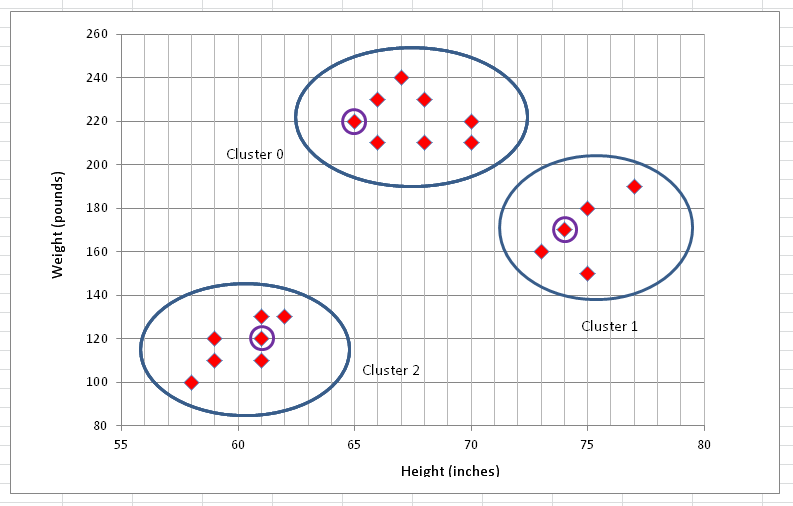
\includegraphics{img/kmedoid.png}
\caption{kmedoid}
\end{figure}

Dalam notasi \emph{pseudocode}, algoritma \emph{KMedoid} adalah sebagai
berikut.

\begin{verbatim}
choose_initial_centroid()
REPEAT
    FOREACH object
        assign_to_cluster(object)
    choose_new_centroid()
    calculate_total_error()
    if (total_error < 0)
        swap(old_centroid, new_centroid)
UNTIL no_changes
\end{verbatim}

    \subsection{Implementation Class}\label{implementation-class}

    \begin{Verbatim}[commandchars=\\\{\}]
{\color{incolor}In [{\color{incolor}18}]:} \PY{k+kn}{import} \PY{n+nn}{numpy} \PY{k}{as} \PY{n+nn}{np}
         \PY{k+kn}{import} \PY{n+nn}{math}
         \PY{k+kn}{import} \PY{n+nn}{random}
         
         \PY{k}{class} \PY{n+nc}{KMedoid}\PY{p}{:}
             \PY{l+s+sd}{\PYZsq{}\PYZsq{}\PYZsq{}}
         \PY{l+s+sd}{    Kelas untuk mengakomodasi nilai metode KMedoid clustering}
         \PY{l+s+sd}{    \PYZsq{}\PYZsq{}\PYZsq{}}
             \PY{c+c1}{\PYZsh{} Nilai default parameter}
             \PY{n}{n\PYZus{}clusters} \PY{o}{=} \PY{l+m+mi}{2}
             \PY{n}{init} \PY{o}{=} \PY{l+s+s1}{\PYZsq{}}\PY{l+s+s1}{random}\PY{l+s+s1}{\PYZsq{}}
             \PY{n}{max\PYZus{}iter} \PY{o}{=} \PY{l+m+mi}{300}
             \PY{n}{init\PYZus{}val} \PY{o}{=} \PY{p}{[}\PY{p}{]}
             \PY{n}{randomize\PYZus{}cluster} \PY{o}{=} \PY{l+m+mi}{0}
             \PY{n}{choosen\PYZus{}cluster} \PY{o}{=} \PY{p}{[}\PY{p}{]}
             
             \PY{n}{available\PYZus{}init} \PY{o}{=} \PY{p}{[}\PY{l+s+s1}{\PYZsq{}}\PY{l+s+s1}{random}\PY{l+s+s1}{\PYZsq{}}\PY{p}{,} \PY{l+s+s1}{\PYZsq{}}\PY{l+s+s1}{manual}\PY{l+s+s1}{\PYZsq{}}\PY{p}{]}
             
             \PY{k}{def} \PY{n+nf}{\PYZus{}\PYZus{}init\PYZus{}\PYZus{}}\PY{p}{(}\PY{n+nb+bp}{self}\PY{p}{,} \PY{n}{n\PYZus{}clusters}\PY{o}{=}\PY{n}{n\PYZus{}clusters}\PY{p}{,} \PY{n}{init}\PY{o}{=}\PY{n}{init}\PY{p}{,} \PY{n}{init\PYZus{}val}\PY{o}{=}\PY{n}{init\PYZus{}val}\PY{p}{,}
                          \PY{n}{max\PYZus{}iter}\PY{o}{=}\PY{n}{max\PYZus{}iter}\PY{p}{,} \PY{n}{randomize\PYZus{}cluster}\PY{o}{=}\PY{n}{randomize\PYZus{}cluster}\PY{p}{)}\PY{p}{:}
                 \PY{l+s+sd}{\PYZsq{}\PYZsq{}\PYZsq{}}
         \PY{l+s+sd}{        Inisiasi kelas. Parameter yang dibutuhkan untuk setiap kelas diinisiasi atau diisi dengan nilai default }
         \PY{l+s+sd}{        \PYZsq{}\PYZsq{}\PYZsq{}}
                 \PY{k}{if} \PY{n}{n\PYZus{}clusters} \PY{o}{\PYZlt{}}\PY{o}{=} \PY{l+m+mi}{0}\PY{p}{:}
                     \PY{k}{raise} \PY{n+ne}{Exception}\PY{p}{(}\PY{l+s+s1}{\PYZsq{}}\PY{l+s+s1}{n\PYZus{}clusters must be higher than 0}\PY{l+s+s1}{\PYZsq{}}\PY{p}{)}
                 \PY{k}{if} \PY{n}{init} \PY{o+ow}{not} \PY{o+ow}{in} \PY{n+nb+bp}{self}\PY{o}{.}\PY{n}{available\PYZus{}init}\PY{p}{:}
                     \PY{k}{raise} \PY{n+ne}{Exception}\PY{p}{(}\PY{l+s+s1}{\PYZsq{}}\PY{l+s+s1}{No init method }\PY{l+s+se}{\PYZbs{}\PYZsq{}}\PY{l+s+s1}{\PYZsq{}} \PY{o}{+} \PY{n+nb}{str}\PY{p}{(}\PY{n}{init}\PY{p}{)} \PY{o}{+} \PY{l+s+s1}{\PYZsq{}}\PY{l+s+se}{\PYZbs{}\PYZsq{}}\PY{l+s+s1}{. Available init methods}\PY{l+s+s1}{\PYZsq{}}\PY{o}{+} \PY{n+nb}{str}\PY{p}{(}\PY{n+nb+bp}{self}\PY{o}{.}\PY{n}{available\PYZus{}init}\PY{p}{)}\PY{p}{)}
                 \PY{k}{if} \PY{p}{(}\PY{n}{init} \PY{o}{==} \PY{l+s+s1}{\PYZsq{}}\PY{l+s+s1}{manual}\PY{l+s+s1}{\PYZsq{}} \PY{o+ow}{and} \PY{n+nb}{len}\PY{p}{(}\PY{n}{init\PYZus{}val}\PY{p}{)} \PY{o}{!=} \PY{n}{n\PYZus{}clusters}\PY{p}{)}\PY{p}{:}
                     \PY{k}{raise} \PY{n+ne}{Exception}\PY{p}{(}\PY{l+s+s1}{\PYZsq{}}\PY{l+s+s1}{init\PYZus{}val length doesn}\PY{l+s+se}{\PYZbs{}\PYZsq{}}\PY{l+s+s1}{t match with n\PYZus{}clusters }\PY{l+s+s1}{\PYZsq{}}\PY{o}{+} \PY{n+nb}{str}\PY{p}{(}\PY{n}{n\PYZus{}clusters}\PY{p}{)}\PY{p}{)}
                 \PY{k}{if} \PY{p}{(}\PY{n}{n\PYZus{}clusters}\PY{o}{\PYZhy{}}\PY{l+m+mi}{1} \PY{o}{\PYZlt{}} \PY{n}{randomize\PYZus{}cluster}\PY{p}{)} \PY{o+ow}{or} \PY{p}{(}\PY{n}{randomize\PYZus{}cluster} \PY{o}{\PYZlt{}} \PY{l+m+mi}{0}\PY{p}{)}\PY{p}{:}
                     \PY{k}{raise} \PY{n+ne}{Exception}\PY{p}{(}\PY{l+s+s1}{\PYZsq{}}\PY{l+s+s1}{randomize\PYZus{}cluster must be between 0 and n\PYZus{}clusters\PYZhy{}1}\PY{l+s+s1}{\PYZsq{}}\PY{p}{)}
                 \PY{n+nb+bp}{self}\PY{o}{.}\PY{n}{n\PYZus{}clusters} \PY{o}{=} \PY{n}{n\PYZus{}clusters}
                 \PY{n+nb+bp}{self}\PY{o}{.}\PY{n}{init} \PY{o}{=} \PY{n}{init}
                 \PY{n+nb+bp}{self}\PY{o}{.}\PY{n}{max\PYZus{}iter} \PY{o}{=} \PY{n}{max\PYZus{}iter}
                 \PY{n+nb+bp}{self}\PY{o}{.}\PY{n}{init\PYZus{}val} \PY{o}{=} \PY{n}{init\PYZus{}val}
                 \PY{n+nb+bp}{self}\PY{o}{.}\PY{n}{randomize\PYZus{}cluster} \PY{o}{=} \PY{n}{randomize\PYZus{}cluster}
             
             \PY{k}{def} \PY{n+nf}{\PYZus{}\PYZus{}is\PYZus{}in\PYZus{}array}\PY{p}{(}\PY{n+nb+bp}{self}\PY{p}{,} \PY{n}{data}\PY{p}{,} \PY{n}{arr}\PY{p}{)}\PY{p}{:}
                 \PY{l+s+sd}{\PYZsq{}\PYZsq{}\PYZsq{}}
         \PY{l+s+sd}{        Fungsi helper untuk menegecek apakah data berupa array berada pada arr berupa array of array}
         \PY{l+s+sd}{        \PYZsq{}\PYZsq{}\PYZsq{}}
                 \PY{n}{is\PYZus{}exist} \PY{o}{=} \PY{k+kc}{False}
                 \PY{n}{arr\PYZus{}idx} \PY{o}{=} \PY{l+m+mi}{0}
                 \PY{k}{while} \PY{p}{(}\PY{o+ow}{not} \PY{n}{is\PYZus{}exist} \PY{o+ow}{and} \PY{n}{arr\PYZus{}idx} \PY{o}{\PYZlt{}} \PY{n+nb}{len}\PY{p}{(}\PY{n}{arr}\PY{p}{)}\PY{p}{)}\PY{p}{:}
                     \PY{n}{is\PYZus{}data\PYZus{}equal} \PY{o}{=} \PY{k+kc}{True}
                     \PY{n}{data\PYZus{}idx} \PY{o}{=} \PY{l+m+mi}{0}
                     \PY{k}{while} \PY{p}{(}\PY{n}{is\PYZus{}data\PYZus{}equal} \PY{o+ow}{and} \PY{n}{data\PYZus{}idx} \PY{o}{\PYZlt{}} \PY{n+nb}{len}\PY{p}{(}\PY{n}{data}\PY{p}{)}\PY{p}{)}\PY{p}{:}
                         \PY{k}{if} \PY{p}{(}\PY{n}{data}\PY{p}{[}\PY{n}{data\PYZus{}idx}\PY{p}{]} \PY{o}{!=} \PY{n}{arr}\PY{p}{[}\PY{n}{arr\PYZus{}idx}\PY{p}{]}\PY{p}{[}\PY{n}{data\PYZus{}idx}\PY{p}{]}\PY{p}{)}\PY{p}{:}
                             \PY{n}{is\PYZus{}data\PYZus{}equal} \PY{o}{=} \PY{k+kc}{False}
                         \PY{k}{else}\PY{p}{:}
                             \PY{n}{data\PYZus{}idx} \PY{o}{+}\PY{o}{=} \PY{l+m+mi}{1}
                     \PY{k}{if} \PY{n}{is\PYZus{}data\PYZus{}equal}\PY{p}{:}
                         \PY{n}{is\PYZus{}exist} \PY{o}{=} \PY{k+kc}{True}
                     \PY{k}{else}\PY{p}{:}
                         \PY{n}{arr\PYZus{}idx} \PY{o}{+}\PY{o}{=} \PY{l+m+mi}{1}
                 \PY{k}{return} \PY{n}{is\PYZus{}exist}
                 
             \PY{k}{def} \PY{n+nf}{\PYZus{}\PYZus{}manhattan\PYZus{}distance}\PY{p}{(}\PY{n+nb+bp}{self}\PY{p}{,} \PY{n}{data1}\PY{p}{,} \PY{n}{data2}\PY{p}{)}\PY{p}{:}
                 \PY{l+s+sd}{\PYZsq{}\PYZsq{}\PYZsq{}}
         \PY{l+s+sd}{        Fungsi untuk menghitung manhattan distance di antara dua vector dengan panjang yang sama}
         \PY{l+s+sd}{        \PYZsq{}\PYZsq{}\PYZsq{}}
                 \PY{n+nb}{sum} \PY{o}{=} \PY{l+m+mi}{0}
                 \PY{k}{if} \PY{p}{(}\PY{n+nb}{len}\PY{p}{(}\PY{n}{data1}\PY{p}{)} \PY{o}{==} \PY{n+nb}{len}\PY{p}{(}\PY{n}{data2}\PY{p}{)}\PY{p}{)}\PY{p}{:}
                     \PY{k}{for} \PY{n}{x1}\PY{p}{,} \PY{n}{x2} \PY{o+ow}{in} \PY{n+nb}{zip}\PY{p}{(}\PY{n}{data1}\PY{p}{,} \PY{n}{data2}\PY{p}{)}\PY{p}{:}
                         \PY{n+nb}{sum} \PY{o}{+}\PY{o}{=} \PY{n+nb}{abs}\PY{p}{(}\PY{n}{x1} \PY{o}{\PYZhy{}} \PY{n}{x2}\PY{p}{)}
                     \PY{k}{return} \PY{n+nb}{sum}
                 \PY{k}{else}\PY{p}{:}
                     \PY{k}{raise} \PY{n+ne}{Exception}\PY{p}{(}\PY{l+s+s1}{\PYZsq{}}\PY{l+s+s1}{Length doesn}\PY{l+s+se}{\PYZbs{}\PYZsq{}}\PY{l+s+s1}{t match}\PY{l+s+s1}{\PYZsq{}}\PY{p}{)}
                     
             \PY{k}{def} \PY{n+nf}{\PYZus{}\PYZus{}get\PYZus{}distance}\PY{p}{(}\PY{n+nb+bp}{self}\PY{p}{,} \PY{n}{data1}\PY{p}{,} \PY{n}{data2}\PY{p}{)}\PY{p}{:}
                 \PY{l+s+sd}{\PYZsq{}\PYZsq{}\PYZsq{}}
         \PY{l+s+sd}{        Fungsi untuk menghitung jarak dua vector}
         \PY{l+s+sd}{        \PYZsq{}\PYZsq{}\PYZsq{}}
                 \PY{k}{return} \PY{n+nb+bp}{self}\PY{o}{.}\PY{n}{\PYZus{}\PYZus{}manhattan\PYZus{}distance}\PY{p}{(}\PY{n}{data1}\PY{p}{,} \PY{n}{data2}\PY{p}{)}
                 
             \PY{k}{def} \PY{n+nf}{\PYZus{}\PYZus{}calculate\PYZus{}distance\PYZus{}matrix}\PY{p}{(}\PY{n+nb+bp}{self}\PY{p}{,} \PY{n}{data}\PY{p}{,} \PY{n}{centroids}\PY{p}{)}\PY{p}{:}
                 \PY{l+s+sd}{\PYZsq{}\PYZsq{}\PYZsq{}}
         \PY{l+s+sd}{        Fungsi untuk menghitung distance matrix untuk semua data dengan centroid}
         \PY{l+s+sd}{        \PYZsq{}\PYZsq{}\PYZsq{}}
                 \PY{n}{dist\PYZus{}matrix} \PY{o}{=} \PY{p}{[}\PY{p}{]}        
                 \PY{k}{for} \PY{n}{i} \PY{o+ow}{in} \PY{n+nb}{range}\PY{p}{(}\PY{n+nb}{len}\PY{p}{(}\PY{n}{centroids}\PY{p}{)}\PY{p}{)}\PY{p}{:}
                     \PY{n}{dist\PYZus{}curr\PYZus{}centroid} \PY{o}{=} \PY{p}{[}\PY{p}{]}
                     \PY{k}{for} \PY{n}{j} \PY{o+ow}{in} \PY{n+nb}{range}\PY{p}{(}\PY{n+nb}{len}\PY{p}{(}\PY{n}{data}\PY{p}{)}\PY{p}{)}\PY{p}{:}
                         \PY{n}{dist} \PY{o}{=} \PY{n+nb+bp}{self}\PY{o}{.}\PY{n}{\PYZus{}\PYZus{}get\PYZus{}distance}\PY{p}{(}\PY{n}{centroids}\PY{p}{[}\PY{n}{i}\PY{p}{]}\PY{p}{,} \PY{n}{data}\PY{p}{[}\PY{n}{j}\PY{p}{]}\PY{p}{)}
                         \PY{n}{dist\PYZus{}curr\PYZus{}centroid}\PY{o}{.}\PY{n}{append}\PY{p}{(}\PY{n}{dist}\PY{p}{)}
                     \PY{n}{dist\PYZus{}matrix}\PY{o}{.}\PY{n}{append}\PY{p}{(}\PY{n}{dist\PYZus{}curr\PYZus{}centroid}\PY{p}{)}
                 
                 \PY{k}{return} \PY{n}{dist\PYZus{}matrix}
             
             \PY{k}{def} \PY{n+nf}{\PYZus{}\PYZus{}assign\PYZus{}data\PYZus{}to\PYZus{}cluster}\PY{p}{(}\PY{n+nb+bp}{self}\PY{p}{,} \PY{n}{dist\PYZus{}matrix}\PY{p}{)}\PY{p}{:}
                 \PY{l+s+sd}{\PYZsq{}\PYZsq{}\PYZsq{}}
         \PY{l+s+sd}{        Fungsi untuk mengelompokan data berdasarkan jarak yang diketahui}
         \PY{l+s+sd}{        \PYZsq{}\PYZsq{}\PYZsq{}}
                 \PY{n}{cluster\PYZus{}of\PYZus{}data} \PY{o}{=} \PY{p}{[}\PY{p}{]}
                 \PY{k}{for} \PY{n}{j} \PY{o+ow}{in} \PY{n+nb}{range}\PY{p}{(}\PY{n+nb}{len}\PY{p}{(}\PY{n}{dist\PYZus{}matrix}\PY{p}{[}\PY{l+m+mi}{0}\PY{p}{]}\PY{p}{)}\PY{p}{)}\PY{p}{:}
                     \PY{n}{cluster} \PY{o}{=} \PY{l+m+mi}{0}
                     \PY{n}{min\PYZus{}distance} \PY{o}{=} \PY{n}{dist\PYZus{}matrix}\PY{p}{[}\PY{l+m+mi}{0}\PY{p}{]}\PY{p}{[}\PY{n}{j}\PY{p}{]}
                     \PY{k}{for} \PY{n}{i} \PY{o+ow}{in} \PY{n+nb}{range}\PY{p}{(}\PY{l+m+mi}{1}\PY{p}{,}\PY{n+nb}{len}\PY{p}{(}\PY{n}{dist\PYZus{}matrix}\PY{p}{)}\PY{p}{)}\PY{p}{:}
                         \PY{k}{if} \PY{p}{(}\PY{n}{dist\PYZus{}matrix}\PY{p}{[}\PY{n}{i}\PY{p}{]}\PY{p}{[}\PY{n}{j}\PY{p}{]} \PY{o}{\PYZlt{}} \PY{n}{min\PYZus{}distance}\PY{p}{)}\PY{p}{:}
                             \PY{n}{cluster} \PY{o}{=} \PY{n}{i}
                             \PY{n}{min\PYZus{}distance} \PY{o}{=} \PY{n}{dist\PYZus{}matrix}\PY{p}{[}\PY{n}{i}\PY{p}{]}\PY{p}{[}\PY{n}{j}\PY{p}{]}
                     \PY{n}{cluster\PYZus{}of\PYZus{}data}\PY{o}{.}\PY{n}{append}\PY{p}{(}\PY{n}{cluster}\PY{p}{)}
                 \PY{k}{return} \PY{n}{cluster\PYZus{}of\PYZus{}data}
             
             \PY{k}{def} \PY{n+nf}{\PYZus{}\PYZus{}get\PYZus{}centroids}\PY{p}{(}\PY{n+nb+bp}{self}\PY{p}{,} \PY{n}{data}\PY{p}{,} \PY{n}{cluster\PYZus{}of\PYZus{}data}\PY{p}{,} \PY{n}{centroids}\PY{p}{)}\PY{p}{:}
                 \PY{l+s+sd}{\PYZsq{}\PYZsq{}\PYZsq{}}
         \PY{l+s+sd}{        Fungsi untuk mendapatkan centroid baru}
         \PY{l+s+sd}{        \PYZsq{}\PYZsq{}\PYZsq{}}
                 \PY{c+c1}{\PYZsh{} centroid candidate}
                 \PY{n}{data\PYZus{}of\PYZus{}randomize\PYZus{}cluster} \PY{o}{=} \PY{p}{[}\PY{p}{]}
                 \PY{k}{for} \PY{n}{idx}\PY{p}{,} \PY{n}{data\PYZus{}cluster} \PY{o+ow}{in} \PY{n+nb}{enumerate}\PY{p}{(}\PY{n}{cluster\PYZus{}of\PYZus{}data}\PY{p}{)}\PY{p}{:}
                     \PY{k}{if} \PY{n}{data\PYZus{}cluster} \PY{o}{==} \PY{n+nb+bp}{self}\PY{o}{.}\PY{n}{randomize\PYZus{}cluster}\PY{p}{:}
                         \PY{n}{data\PYZus{}of\PYZus{}randomize\PYZus{}cluster}\PY{o}{.}\PY{n}{append}\PY{p}{(}\PY{n}{data}\PY{p}{[}\PY{n}{idx}\PY{p}{]}\PY{p}{)}
                 
                 \PY{c+c1}{\PYZsh{} choose random}
                 \PY{n}{idx} \PY{o}{=} \PY{l+m+mi}{0}
                 \PY{n}{stop} \PY{o}{=} \PY{k+kc}{False}
                 \PY{k}{while} \PY{p}{(} \PY{o+ow}{not} \PY{n}{stop} \PY{o+ow}{and} \PY{n}{idx} \PY{o}{\PYZlt{}} \PY{n+nb}{len}\PY{p}{(}\PY{n}{data\PYZus{}of\PYZus{}randomize\PYZus{}cluster}\PY{p}{)}
                 \PY{p}{)}\PY{p}{:}
                     \PY{n}{new\PYZus{}centroid} \PY{o}{=} \PY{n}{np}\PY{o}{.}\PY{n}{copy}\PY{p}{(}\PY{n}{data\PYZus{}of\PYZus{}randomize\PYZus{}cluster}\PY{p}{[}\PY{n}{idx}\PY{p}{]}\PY{p}{)}
                     \PY{k}{if} \PY{p}{(}
                         \PY{n+nb+bp}{self}\PY{o}{.}\PY{n}{\PYZus{}\PYZus{}get\PYZus{}distance}\PY{p}{(}\PY{n}{new\PYZus{}centroid}\PY{p}{,} \PY{n}{centroids}\PY{p}{[}\PY{n+nb+bp}{self}\PY{o}{.}\PY{n}{randomize\PYZus{}cluster}\PY{p}{]}\PY{p}{)} \PY{o}{==} \PY{l+m+mi}{0} \PY{o+ow}{or} 
                         \PY{n+nb+bp}{self}\PY{o}{.}\PY{n}{\PYZus{}\PYZus{}is\PYZus{}in\PYZus{}array}\PY{p}{(}\PY{n}{new\PYZus{}centroid}\PY{p}{,} \PY{n+nb+bp}{self}\PY{o}{.}\PY{n}{choosen\PYZus{}cluster}\PY{p}{)}
                     \PY{p}{)}\PY{p}{:}
                         \PY{n}{idx} \PY{o}{+}\PY{o}{=} \PY{l+m+mi}{1}
                     \PY{k}{else}\PY{p}{:}
                         \PY{n}{stop} \PY{o}{=} \PY{k+kc}{True}
                 
                 \PY{k}{if} \PY{o+ow}{not} \PY{n+nb+bp}{self}\PY{o}{.}\PY{n}{\PYZus{}\PYZus{}is\PYZus{}in\PYZus{}array}\PY{p}{(}\PY{n}{new\PYZus{}centroid}\PY{p}{,} \PY{n+nb+bp}{self}\PY{o}{.}\PY{n}{choosen\PYZus{}cluster}\PY{p}{)}\PY{p}{:}
                     \PY{n+nb+bp}{self}\PY{o}{.}\PY{n}{choosen\PYZus{}cluster}\PY{o}{.}\PY{n}{append}\PY{p}{(}\PY{n}{new\PYZus{}centroid}\PY{p}{)}
                 
                 \PY{n}{new\PYZus{}centroids} \PY{o}{=} \PY{n}{np}\PY{o}{.}\PY{n}{copy}\PY{p}{(}\PY{n}{centroids}\PY{p}{)}
                 \PY{n}{new\PYZus{}centroids}\PY{p}{[}\PY{n+nb+bp}{self}\PY{o}{.}\PY{n}{randomize\PYZus{}cluster}\PY{p}{]} \PY{o}{=} \PY{n}{new\PYZus{}centroid}
                 \PY{k}{return} \PY{n}{new\PYZus{}centroids}
             
             \PY{k}{def} \PY{n+nf}{\PYZus{}\PYZus{}calculate\PYZus{}error}\PY{p}{(}\PY{n+nb+bp}{self}\PY{p}{,} \PY{n}{data}\PY{p}{,} \PY{n}{cluster\PYZus{}of\PYZus{}data}\PY{p}{,} \PY{n}{new\PYZus{}cluster\PYZus{}of\PYZus{}data}\PY{p}{,} \PY{n}{centroids}\PY{p}{,} \PY{n}{new\PYZus{}centroids}\PY{p}{)}\PY{p}{:}
                 \PY{l+s+sd}{\PYZsq{}\PYZsq{}\PYZsq{}}
         \PY{l+s+sd}{        Fungsi untuk menghitung total absolute error}
         \PY{l+s+sd}{        \PYZsq{}\PYZsq{}\PYZsq{}}
                 
                 \PY{n}{old\PYZus{}error} \PY{o}{=} \PY{l+m+mi}{0}
                 \PY{n}{new\PYZus{}error} \PY{o}{=} \PY{l+m+mi}{0}
                 \PY{k}{for} \PY{n}{n} \PY{o+ow}{in} \PY{n+nb}{range}\PY{p}{(}\PY{n+nb+bp}{self}\PY{o}{.}\PY{n}{n\PYZus{}clusters}\PY{p}{)}\PY{p}{:}
                     \PY{k}{for} \PY{n}{idx}\PY{p}{,} \PY{n}{val} \PY{o+ow}{in} \PY{n+nb}{enumerate}\PY{p}{(}\PY{n}{data}\PY{p}{)}\PY{p}{:}
                         \PY{n}{old\PYZus{}error} \PY{o}{+}\PY{o}{=} \PY{n+nb+bp}{self}\PY{o}{.}\PY{n}{\PYZus{}\PYZus{}get\PYZus{}distance}\PY{p}{(}\PY{n}{val}\PY{p}{,} \PY{n}{centroids}\PY{p}{[}\PY{n}{cluster\PYZus{}of\PYZus{}data}\PY{p}{[}\PY{n}{idx}\PY{p}{]}\PY{p}{]}\PY{p}{)}
                         \PY{n}{new\PYZus{}error} \PY{o}{+}\PY{o}{=} \PY{n+nb+bp}{self}\PY{o}{.}\PY{n}{\PYZus{}\PYZus{}get\PYZus{}distance}\PY{p}{(}\PY{n}{val}\PY{p}{,} \PY{n}{new\PYZus{}centroids}\PY{p}{[}\PY{n}{new\PYZus{}cluster\PYZus{}of\PYZus{}data}\PY{p}{[}\PY{n}{idx}\PY{p}{]}\PY{p}{]}\PY{p}{)}
                 
                 \PY{k}{return} \PY{n}{new\PYZus{}error}\PY{o}{\PYZhy{}}\PY{n}{old\PYZus{}error}
                 
             \PY{k}{def} \PY{n+nf}{fit\PYZus{}predict}\PY{p}{(}\PY{n+nb+bp}{self}\PY{p}{,} \PY{n}{data}\PY{p}{)}\PY{p}{:}
                 \PY{l+s+sd}{\PYZsq{}\PYZsq{}\PYZsq{}}
         \PY{l+s+sd}{        Fungsi untuk melakukan clustering secara KMedoid}
         \PY{l+s+sd}{        \PYZsq{}\PYZsq{}\PYZsq{}}
                 
                 \PY{n}{cluster\PYZus{}of\PYZus{}data} \PY{o}{=} \PY{p}{[}\PY{p}{]}
                 
                 \PY{c+c1}{\PYZsh{} initiate centroid}
                 \PY{n}{centroids} \PY{o}{=} \PY{p}{[}\PY{p}{]}
                 \PY{k}{if} \PY{p}{(}\PY{n+nb+bp}{self}\PY{o}{.}\PY{n}{init} \PY{o}{==} \PY{l+s+s1}{\PYZsq{}}\PY{l+s+s1}{random}\PY{l+s+s1}{\PYZsq{}}\PY{p}{)}\PY{p}{:}
                     \PY{c+c1}{\PYZsh{} cek keunikan data}
                     \PY{n}{unique\PYZus{}data\PYZus{}idx} \PY{o}{=} \PY{p}{[}\PY{p}{]}
                     \PY{n}{unique\PYZus{}data} \PY{o}{=} \PY{p}{[}\PY{p}{]}
                     \PY{n}{i} \PY{o}{=} \PY{l+m+mi}{0}
                     \PY{k}{while} \PY{p}{(}\PY{n+nb}{len}\PY{p}{(}\PY{n}{unique\PYZus{}data\PYZus{}idx}\PY{p}{)} \PY{o}{\PYZlt{}} \PY{n+nb+bp}{self}\PY{o}{.}\PY{n}{n\PYZus{}clusters}\PY{p}{)} \PY{o+ow}{and} \PY{p}{(}\PY{n}{i} \PY{o}{\PYZlt{}} \PY{n+nb}{len}\PY{p}{(}\PY{n}{data}\PY{p}{)}\PY{p}{)}\PY{p}{:}
                         \PY{k}{if} \PY{o+ow}{not} \PY{n+nb+bp}{self}\PY{o}{.}\PY{n}{\PYZus{}\PYZus{}is\PYZus{}in\PYZus{}array}\PY{p}{(}\PY{n}{data}\PY{p}{[}\PY{n}{i}\PY{p}{]}\PY{p}{,} \PY{n}{unique\PYZus{}data}\PY{p}{)}\PY{p}{:}
                             \PY{n}{unique\PYZus{}data\PYZus{}idx}\PY{o}{.}\PY{n}{append}\PY{p}{(}\PY{n}{i}\PY{p}{)}
                             \PY{n}{unique\PYZus{}data}\PY{o}{.}\PY{n}{append}\PY{p}{(}\PY{n}{data}\PY{p}{[}\PY{n}{i}\PY{p}{]}\PY{p}{)}
                         \PY{n}{i} \PY{o}{+}\PY{o}{=} \PY{l+m+mi}{1}
                         
                     \PY{k}{if} \PY{p}{(}\PY{n+nb}{len}\PY{p}{(}\PY{n}{unique\PYZus{}data\PYZus{}idx}\PY{p}{)} \PY{o}{\PYZlt{}} \PY{n+nb+bp}{self}\PY{o}{.}\PY{n}{n\PYZus{}clusters}\PY{p}{)}\PY{p}{:}
                         \PY{c+c1}{\PYZsh{} jika keunikan data kurang dari n\PYZus{}clusters}
                         \PY{k}{for} \PY{n}{u} \PY{o+ow}{in} \PY{n}{unique\PYZus{}data\PYZus{}idx}\PY{p}{:}
                             \PY{n}{curr\PYZus{}centroid} \PY{o}{=} \PY{n}{np}\PY{o}{.}\PY{n}{copy}\PY{p}{(}\PY{n}{data}\PY{p}{[}\PY{n}{u}\PY{p}{]}\PY{p}{)}
                             \PY{n}{centroids}\PY{o}{.}\PY{n}{append}\PY{p}{(}\PY{n}{curr\PYZus{}centroid}\PY{p}{)}
                         \PY{k}{for} \PY{n}{i} \PY{o+ow}{in} \PY{n+nb}{range}\PY{p}{(}\PY{n+nb+bp}{self}\PY{o}{.}\PY{n}{n\PYZus{}clusters} \PY{o}{\PYZhy{}} \PY{n+nb}{len}\PY{p}{(}\PY{n}{unique\PYZus{}data\PYZus{}idx}\PY{p}{)}\PY{p}{)}\PY{p}{:}
                             \PY{n}{rand\PYZus{}idx} \PY{o}{=} \PY{n}{random}\PY{o}{.}\PY{n}{randint}\PY{p}{(}\PY{o}{\PYZhy{}}\PY{l+m+mi}{1}\PY{p}{,}\PY{n+nb}{len}\PY{p}{(}\PY{n}{data}\PY{p}{)}\PY{o}{\PYZhy{}}\PY{l+m+mi}{1}\PY{p}{)}
                             \PY{c+c1}{\PYZsh{} cek apakah sudah terpilih atau belum}
                             \PY{k}{while} \PY{p}{(}\PY{n}{rand\PYZus{}idx} \PY{o+ow}{in} \PY{n}{unique\PYZus{}data\PYZus{}idx}\PY{p}{)}\PY{p}{:}
                                 \PY{n}{rand\PYZus{}idx} \PY{o}{=} \PY{n}{random}\PY{o}{.}\PY{n}{randint}\PY{p}{(}\PY{o}{\PYZhy{}}\PY{l+m+mi}{1}\PY{p}{,}\PY{n+nb}{len}\PY{p}{(}\PY{n}{data}\PY{p}{)}\PY{o}{\PYZhy{}}\PY{l+m+mi}{1}\PY{p}{)}
                             \PY{n}{curr\PYZus{}centroid} \PY{o}{=} \PY{n}{np}\PY{o}{.}\PY{n}{copy}\PY{p}{(}\PY{n}{data}\PY{p}{[}\PY{n}{rand\PYZus{}idx}\PY{p}{]}\PY{p}{)}
                             \PY{n}{centroids}\PY{o}{.}\PY{n}{append}\PY{p}{(}\PY{n}{curr\PYZus{}centroid}\PY{p}{)}
                     \PY{k}{else}\PY{p}{:}
                         \PY{k}{for} \PY{n}{i} \PY{o+ow}{in} \PY{n+nb}{range}\PY{p}{(}\PY{n+nb+bp}{self}\PY{o}{.}\PY{n}{n\PYZus{}clusters}\PY{p}{)}\PY{p}{:}
                             \PY{n}{rand\PYZus{}idx} \PY{o}{=} \PY{n}{random}\PY{o}{.}\PY{n}{randint}\PY{p}{(}\PY{o}{\PYZhy{}}\PY{l+m+mi}{1}\PY{p}{,}\PY{n+nb}{len}\PY{p}{(}\PY{n}{data}\PY{p}{)}\PY{o}{\PYZhy{}}\PY{l+m+mi}{1}\PY{p}{)}
                             \PY{n}{curr\PYZus{}centroid} \PY{o}{=} \PY{n}{np}\PY{o}{.}\PY{n}{copy}\PY{p}{(}\PY{n}{data}\PY{p}{[}\PY{n}{rand\PYZus{}idx}\PY{p}{]}\PY{p}{)}
                             \PY{c+c1}{\PYZsh{} cek apakah sudah terpilih atau belum}
                             \PY{k}{while} \PY{p}{(}\PY{n+nb+bp}{self}\PY{o}{.}\PY{n}{\PYZus{}\PYZus{}is\PYZus{}in\PYZus{}array}\PY{p}{(}\PY{n}{curr\PYZus{}centroid}\PY{p}{,} \PY{n}{centroids}\PY{p}{)}\PY{p}{)}\PY{p}{:}
                                 \PY{n}{rand\PYZus{}idx} \PY{o}{=} \PY{n}{random}\PY{o}{.}\PY{n}{randint}\PY{p}{(}\PY{o}{\PYZhy{}}\PY{l+m+mi}{1}\PY{p}{,}\PY{n+nb}{len}\PY{p}{(}\PY{n}{data}\PY{p}{)}\PY{o}{\PYZhy{}}\PY{l+m+mi}{1}\PY{p}{)}
                                 \PY{n}{curr\PYZus{}centroid} \PY{o}{=} \PY{n}{np}\PY{o}{.}\PY{n}{copy}\PY{p}{(}\PY{n}{data}\PY{p}{[}\PY{n}{rand\PYZus{}idx}\PY{p}{]}\PY{p}{)}
                             \PY{n}{centroids}\PY{o}{.}\PY{n}{append}\PY{p}{(}\PY{n}{curr\PYZus{}centroid}\PY{p}{)}
                 \PY{k}{else}\PY{p}{:}
                     \PY{c+c1}{\PYZsh{} self.init == \PYZsq{}manual\PYZsq{}}
                     \PY{n}{centroids} \PY{o}{=} \PY{n+nb+bp}{self}\PY{o}{.}\PY{n}{init\PYZus{}val}
                 
                 \PY{n}{iteration} \PY{o}{=} \PY{l+m+mi}{1}
                 \PY{n}{is\PYZus{}convergen} \PY{o}{=} \PY{k+kc}{False}
                 
                 \PY{k}{while} \PY{p}{(}\PY{o+ow}{not} \PY{n}{is\PYZus{}convergen} \PY{o+ow}{and} \PY{n}{iteration} \PY{o}{\PYZlt{}}\PY{o}{=} \PY{n+nb+bp}{self}\PY{o}{.}\PY{n}{max\PYZus{}iter}\PY{p}{)}\PY{p}{:}
                     \PY{c+c1}{\PYZsh{} calculate distance all data to all centroid}
                     \PY{n}{dist\PYZus{}matrix} \PY{o}{=} \PY{n+nb+bp}{self}\PY{o}{.}\PY{n}{\PYZus{}\PYZus{}calculate\PYZus{}distance\PYZus{}matrix}\PY{p}{(}\PY{n}{data}\PY{p}{,} \PY{n}{centroids}\PY{p}{)}
                     \PY{c+c1}{\PYZsh{} assign all data to cluster}
                     \PY{n}{cluster\PYZus{}of\PYZus{}data} \PY{o}{=} \PY{n+nb+bp}{self}\PY{o}{.}\PY{n}{\PYZus{}\PYZus{}assign\PYZus{}data\PYZus{}to\PYZus{}cluster}\PY{p}{(}\PY{n}{dist\PYZus{}matrix}\PY{p}{)}
                     \PY{c+c1}{\PYZsh{} get new possible centroid}
                     \PY{n}{new\PYZus{}centroids} \PY{o}{=} \PY{n+nb+bp}{self}\PY{o}{.}\PY{n}{\PYZus{}\PYZus{}get\PYZus{}centroids}\PY{p}{(}\PY{n}{data}\PY{p}{,} \PY{n}{cluster\PYZus{}of\PYZus{}data}\PY{p}{,} \PY{n}{centroids}\PY{p}{)}
                     \PY{c+c1}{\PYZsh{} calculate distance all data to all new centroid}
                     \PY{n}{new\PYZus{}dist\PYZus{}matrix} \PY{o}{=} \PY{n+nb+bp}{self}\PY{o}{.}\PY{n}{\PYZus{}\PYZus{}calculate\PYZus{}distance\PYZus{}matrix}\PY{p}{(}\PY{n}{data}\PY{p}{,} \PY{n}{new\PYZus{}centroids}\PY{p}{)}
                     \PY{c+c1}{\PYZsh{} assign all data to new cluster}
                     \PY{n}{new\PYZus{}cluster\PYZus{}of\PYZus{}data} \PY{o}{=} \PY{n+nb+bp}{self}\PY{o}{.}\PY{n}{\PYZus{}\PYZus{}assign\PYZus{}data\PYZus{}to\PYZus{}cluster}\PY{p}{(}\PY{n}{new\PYZus{}dist\PYZus{}matrix}\PY{p}{)}
                     \PY{c+c1}{\PYZsh{} convergency checking}
                     \PY{k}{if} \PY{p}{(}\PY{n+nb+bp}{self}\PY{o}{.}\PY{n}{\PYZus{}\PYZus{}calculate\PYZus{}error}\PY{p}{(}\PY{n}{data}\PY{p}{,} \PY{n}{cluster\PYZus{}of\PYZus{}data}\PY{p}{,} \PY{n}{new\PYZus{}cluster\PYZus{}of\PYZus{}data}\PY{p}{,} \PY{n}{centroids}\PY{p}{,} \PY{n}{new\PYZus{}centroids}\PY{p}{)} \PY{o}{\PYZgt{}}\PY{o}{=} \PY{l+m+mi}{0}\PY{p}{)}\PY{p}{:}
                         \PY{n}{is\PYZus{}convergen} \PY{o}{=} \PY{k+kc}{True}
                     
                     \PY{c+c1}{\PYZsh{} for next iteration}
                     \PY{k}{if} \PY{o+ow}{not} \PY{n}{is\PYZus{}convergen}\PY{p}{:}
                         \PY{n}{cluster\PYZus{}of\PYZus{}data} \PY{o}{=} \PY{n}{np}\PY{o}{.}\PY{n}{copy}\PY{p}{(}\PY{n}{new\PYZus{}cluster\PYZus{}of\PYZus{}data}\PY{p}{)}
                         \PY{n}{centroids} \PY{o}{=} \PY{n}{np}\PY{o}{.}\PY{n}{copy}\PY{p}{(}\PY{n}{new\PYZus{}centroids}\PY{p}{)}
                         \PY{n}{iteration} \PY{o}{+}\PY{o}{=} \PY{l+m+mi}{1}
                         
                 \PY{k}{return} \PY{n}{np}\PY{o}{.}\PY{n}{array}\PY{p}{(}\PY{n}{cluster\PYZus{}of\PYZus{}data}\PY{p}{)}
\end{Verbatim}


    \subsection{Experiments}\label{experiments}

Berikut ini merupakan hasil eksperimen implementasi KMedoid (PAM) untuk
clustering data iris

    \paragraph{Clustering dengan k=4,
randomize\_cluster=0}\label{clustering-dengan-k4-randomizeux5fcluster0}

Pada percobaan ini, dipilih nilai k=4 dan randomize\_cluster=0, artinya
cluster yang akan dirandom centroidnya untuk setiap iterasi adalah
cluster pertama. Hasil clustering dan \emph{purity}-nya dapat dilihat
pada \emph{output} dari eksekusi \emph{code}.

    \begin{Verbatim}[commandchars=\\\{\}]
{\color{incolor}In [{\color{incolor}23}]:} \PY{n}{kmedoid} \PY{o}{=} \PY{n}{KMedoid}\PY{p}{(}\PY{n}{n\PYZus{}clusters}\PY{o}{=}\PY{l+m+mi}{4}\PY{p}{,} \PY{n}{randomize\PYZus{}cluster}\PY{o}{=}\PY{l+m+mi}{0}\PY{p}{)}
         \PY{n}{start} \PY{o}{=} \PY{n}{time}\PY{o}{.}\PY{n}{time}\PY{p}{(}\PY{p}{)}
         \PY{n}{pred} \PY{o}{=} \PY{n}{kmedoid}\PY{o}{.}\PY{n}{fit\PYZus{}predict}\PY{p}{(}\PY{n}{data}\PY{p}{)}
         
         \PY{n+nb}{print}\PY{p}{(}\PY{l+s+s2}{\PYZdq{}}\PY{l+s+s2}{\PYZhy{}\PYZhy{}\PYZhy{}\PYZhy{} Time taken: }\PY{l+s+si}{\PYZob{}\PYZcb{}}\PY{l+s+s2}{ s \PYZhy{}\PYZhy{}\PYZhy{}\PYZhy{}}\PY{l+s+s2}{\PYZdq{}}\PY{o}{.}\PY{n}{format}\PY{p}{(}\PY{n}{time}\PY{o}{.}\PY{n}{time}\PY{p}{(}\PY{p}{)} \PY{o}{\PYZhy{}} \PY{n}{start}\PY{p}{)}\PY{p}{)}
         \PY{n+nb}{print}\PY{p}{(}\PY{l+s+s2}{\PYZdq{}}\PY{l+s+s2}{Cluster prediction:}\PY{l+s+s2}{\PYZdq{}}\PY{p}{)}
         \PY{n+nb}{print}\PY{p}{(}\PY{n}{pred}\PY{p}{)}
         \PY{n+nb}{print}\PY{p}{(}\PY{l+s+s2}{\PYZdq{}}\PY{l+s+s2}{Purity: }\PY{l+s+si}{\PYZob{}\PYZcb{}}\PY{l+s+s2}{\PYZdq{}}\PY{o}{.}\PY{n}{format}\PY{p}{(}\PY{n}{purity}\PY{p}{(}\PY{n}{pred}\PY{p}{,} \PY{n}{label}\PY{p}{)}\PY{p}{)}\PY{p}{)}
\end{Verbatim}


    \begin{Verbatim}[commandchars=\\\{\}]
---- Time taken: 0.09967494010925293 s ----
Cluster prediction:
[1 1 1 1 1 1 1 1 1 1 1 1 1 1 1 1 1 1 1 1 1 1 1 1 1 1 1 1 1 1 1 1 1 1 1 1 1
 1 1 1 1 1 1 1 1 1 1 1 1 1 3 3 3 0 0 0 3 0 3 0 0 0 0 0 0 3 0 0 0 0 0 0 0 0
 0 3 3 3 0 0 0 0 0 0 0 0 3 0 0 0 0 0 0 0 0 0 0 0 0 0 2 0 2 2 2 2 0 2 2 2 2
 2 2 0 0 2 2 2 2 0 2 0 2 0 2 2 0 0 2 2 2 2 2 0 0 2 2 2 0 2 2 2 0 2 2 2 0 2
 2 0]
Purity: 0.9

    \end{Verbatim}

    \paragraph{Clustering dengan k=4,
randomize\_cluster=1}\label{clustering-dengan-k4-randomizeux5fcluster1}

Pada percobaan ini, dipilih nilai k=4 dan randomize\_cluster=1, artinya
cluster yang akan dirandom centroidnya untuk setiap iterasi adalah
cluster kedua. Hasil clustering dan \emph{purity}-nya dapat dilihat pada
\emph{output} dari eksekusi \emph{code}.

    \begin{Verbatim}[commandchars=\\\{\}]
{\color{incolor}In [{\color{incolor}20}]:} \PY{n}{kmedoid} \PY{o}{=} \PY{n}{KMedoid}\PY{p}{(}\PY{n}{n\PYZus{}clusters}\PY{o}{=}\PY{l+m+mi}{4}\PY{p}{,} \PY{n}{randomize\PYZus{}cluster}\PY{o}{=}\PY{l+m+mi}{1}\PY{p}{)}
         \PY{n}{start} \PY{o}{=} \PY{n}{time}\PY{o}{.}\PY{n}{time}\PY{p}{(}\PY{p}{)}
         \PY{n}{pred} \PY{o}{=} \PY{n}{kmedoid}\PY{o}{.}\PY{n}{fit\PYZus{}predict}\PY{p}{(}\PY{n}{data}\PY{p}{)}
         
         \PY{n+nb}{print}\PY{p}{(}\PY{l+s+s2}{\PYZdq{}}\PY{l+s+s2}{\PYZhy{}\PYZhy{}\PYZhy{}\PYZhy{} Time taken: }\PY{l+s+si}{\PYZob{}\PYZcb{}}\PY{l+s+s2}{ s \PYZhy{}\PYZhy{}\PYZhy{}\PYZhy{}}\PY{l+s+s2}{\PYZdq{}}\PY{o}{.}\PY{n}{format}\PY{p}{(}\PY{n}{time}\PY{o}{.}\PY{n}{time}\PY{p}{(}\PY{p}{)} \PY{o}{\PYZhy{}} \PY{n}{start}\PY{p}{)}\PY{p}{)}
         \PY{n+nb}{print}\PY{p}{(}\PY{l+s+s2}{\PYZdq{}}\PY{l+s+s2}{Cluster prediction:}\PY{l+s+s2}{\PYZdq{}}\PY{p}{)}
         \PY{n+nb}{print}\PY{p}{(}\PY{n}{pred}\PY{p}{)}
         \PY{n+nb}{print}\PY{p}{(}\PY{l+s+s2}{\PYZdq{}}\PY{l+s+s2}{Purity: }\PY{l+s+si}{\PYZob{}\PYZcb{}}\PY{l+s+s2}{\PYZdq{}}\PY{o}{.}\PY{n}{format}\PY{p}{(}\PY{n}{purity}\PY{p}{(}\PY{n}{pred}\PY{p}{,} \PY{n}{label}\PY{p}{)}\PY{p}{)}\PY{p}{)}
\end{Verbatim}


    \begin{Verbatim}[commandchars=\\\{\}]
---- Time taken: 0.0945584774017334 s ----
Cluster prediction:
[3 0 0 0 3 1 3 3 0 0 1 3 0 0 1 1 1 3 1 3 1 3 3 3 3 0 3 3 3 0 0 1 1 1 0 3 1
 0 0 3 3 0 0 3 3 0 3 0 1 3 2 2 2 2 2 2 2 0 2 2 2 2 2 2 2 2 2 2 2 2 2 2 2 2
 2 2 2 2 2 2 2 2 2 2 2 2 2 2 2 2 2 2 2 0 2 2 2 2 0 2 2 2 2 2 2 2 2 2 2 2 2
 2 2 2 2 2 2 2 2 2 2 2 2 2 2 2 2 2 2 2 2 2 2 2 2 2 2 2 2 2 2 2 2 2 2 2 2 2
 2 2]
Purity: 0.6666666666666666

    \end{Verbatim}

    \paragraph{Clustering dengan k=4,
randomize\_cluster=2}\label{clustering-dengan-k4-randomizeux5fcluster2}

Pada percobaan ini, dipilih nilai k=4 dan randomize\_cluster=2, artinya
cluster yang akan dirandom centroidnya untuk setiap iterasi adalah
cluster ketiga. Hasil clustering dan \emph{purity}-nya dapat dilihat
pada \emph{output} dari eksekusi \emph{code}.

    \begin{Verbatim}[commandchars=\\\{\}]
{\color{incolor}In [{\color{incolor}26}]:} \PY{n}{kmedoid} \PY{o}{=} \PY{n}{KMedoid}\PY{p}{(}\PY{n}{n\PYZus{}clusters}\PY{o}{=}\PY{l+m+mi}{4}\PY{p}{,} \PY{n}{randomize\PYZus{}cluster}\PY{o}{=}\PY{l+m+mi}{2}\PY{p}{)}
         \PY{n}{start} \PY{o}{=} \PY{n}{time}\PY{o}{.}\PY{n}{time}\PY{p}{(}\PY{p}{)}
         \PY{n}{pred} \PY{o}{=} \PY{n}{kmedoid}\PY{o}{.}\PY{n}{fit\PYZus{}predict}\PY{p}{(}\PY{n}{data}\PY{p}{)}
         
         \PY{n+nb}{print}\PY{p}{(}\PY{l+s+s2}{\PYZdq{}}\PY{l+s+s2}{\PYZhy{}\PYZhy{}\PYZhy{}\PYZhy{} Time taken: }\PY{l+s+si}{\PYZob{}\PYZcb{}}\PY{l+s+s2}{ s \PYZhy{}\PYZhy{}\PYZhy{}\PYZhy{}}\PY{l+s+s2}{\PYZdq{}}\PY{o}{.}\PY{n}{format}\PY{p}{(}\PY{n}{time}\PY{o}{.}\PY{n}{time}\PY{p}{(}\PY{p}{)} \PY{o}{\PYZhy{}} \PY{n}{start}\PY{p}{)}\PY{p}{)}
         \PY{n+nb}{print}\PY{p}{(}\PY{l+s+s2}{\PYZdq{}}\PY{l+s+s2}{Cluster prediction:}\PY{l+s+s2}{\PYZdq{}}\PY{p}{)}
         \PY{n+nb}{print}\PY{p}{(}\PY{n}{pred}\PY{p}{)}
         \PY{n+nb}{print}\PY{p}{(}\PY{l+s+s2}{\PYZdq{}}\PY{l+s+s2}{Purity: }\PY{l+s+si}{\PYZob{}\PYZcb{}}\PY{l+s+s2}{\PYZdq{}}\PY{o}{.}\PY{n}{format}\PY{p}{(}\PY{n}{purity}\PY{p}{(}\PY{n}{pred}\PY{p}{,} \PY{n}{label}\PY{p}{)}\PY{p}{)}\PY{p}{)}
\end{Verbatim}


    \begin{Verbatim}[commandchars=\\\{\}]
---- Time taken: 0.06009364128112793 s ----
Cluster prediction:
[0 0 0 0 0 0 0 0 0 0 0 0 0 0 0 0 0 0 0 0 0 0 0 0 0 0 0 0 0 0 0 0 0 0 0 0 0
 0 0 0 0 0 0 0 0 0 0 0 0 0 2 2 2 3 2 3 2 3 2 3 3 3 3 2 3 2 2 3 2 3 2 3 2 2
 2 2 2 2 2 3 3 3 3 1 2 2 2 2 3 3 3 2 3 3 3 3 3 2 3 3 1 1 1 1 1 1 1 1 1 1 1
 1 1 1 1 1 1 1 1 2 1 1 1 1 1 1 2 2 1 2 1 1 1 2 2 1 1 1 2 1 1 1 1 1 1 1 1 1
 1 1]
Purity: 0.9466666666666667

    \end{Verbatim}

    \paragraph{Clustering dengan k=4,
randomize\_cluster=3}\label{clustering-dengan-k4-randomizeux5fcluster3}

Pada percobaan ini, dipilih nilai k=4 dan randomize\_cluster=0, artinya
cluster yang akan dirandom centroidnya untuk setiap iterasi adalah
cluster keempat. Hasil clustering dan \emph{purity}-nya dapat dilihat
pada \emph{output} dari eksekusi \emph{code}.

    \begin{Verbatim}[commandchars=\\\{\}]
{\color{incolor}In [{\color{incolor}22}]:} \PY{n}{kmedoid} \PY{o}{=} \PY{n}{KMedoid}\PY{p}{(}\PY{n}{n\PYZus{}clusters}\PY{o}{=}\PY{l+m+mi}{4}\PY{p}{,} \PY{n}{randomize\PYZus{}cluster}\PY{o}{=}\PY{l+m+mi}{3}\PY{p}{)}
         \PY{n}{start} \PY{o}{=} \PY{n}{time}\PY{o}{.}\PY{n}{time}\PY{p}{(}\PY{p}{)}
         \PY{n}{pred} \PY{o}{=} \PY{n}{kmedoid}\PY{o}{.}\PY{n}{fit\PYZus{}predict}\PY{p}{(}\PY{n}{data}\PY{p}{)}
         
         \PY{n+nb}{print}\PY{p}{(}\PY{l+s+s2}{\PYZdq{}}\PY{l+s+s2}{\PYZhy{}\PYZhy{}\PYZhy{}\PYZhy{} Time taken: }\PY{l+s+si}{\PYZob{}\PYZcb{}}\PY{l+s+s2}{ s \PYZhy{}\PYZhy{}\PYZhy{}\PYZhy{}}\PY{l+s+s2}{\PYZdq{}}\PY{o}{.}\PY{n}{format}\PY{p}{(}\PY{n}{time}\PY{o}{.}\PY{n}{time}\PY{p}{(}\PY{p}{)} \PY{o}{\PYZhy{}} \PY{n}{start}\PY{p}{)}\PY{p}{)}
         \PY{n+nb}{print}\PY{p}{(}\PY{l+s+s2}{\PYZdq{}}\PY{l+s+s2}{Cluster prediction:}\PY{l+s+s2}{\PYZdq{}}\PY{p}{)}
         \PY{n+nb}{print}\PY{p}{(}\PY{n}{pred}\PY{p}{)}
         \PY{n+nb}{print}\PY{p}{(}\PY{l+s+s2}{\PYZdq{}}\PY{l+s+s2}{Purity: }\PY{l+s+si}{\PYZob{}\PYZcb{}}\PY{l+s+s2}{\PYZdq{}}\PY{o}{.}\PY{n}{format}\PY{p}{(}\PY{n}{purity}\PY{p}{(}\PY{n}{pred}\PY{p}{,} \PY{n}{label}\PY{p}{)}\PY{p}{)}\PY{p}{)}
\end{Verbatim}


    \begin{Verbatim}[commandchars=\\\{\}]
---- Time taken: 0.05040931701660156 s ----
Cluster prediction:
[1 1 1 1 1 1 1 1 1 1 1 1 1 1 1 1 1 1 1 1 1 1 1 1 1 1 1 1 1 1 1 1 1 1 1 1 1
 1 1 1 1 1 1 1 1 1 1 1 1 1 3 3 3 2 0 2 3 2 3 2 2 2 2 0 2 3 2 2 0 2 3 2 0 2
 0 3 3 3 0 2 2 2 2 0 2 0 3 0 2 2 2 0 2 2 2 2 2 0 2 2 3 2 3 3 3 3 0 3 3 3 3
 3 3 0 2 3 3 3 3 0 3 0 3 0 3 3 0 3 3 3 3 3 3 3 0 3 3 3 3 3 3 3 2 3 3 3 0 3
 3 3]
Purity: 0.8533333333333334

    \end{Verbatim}

    \subsection{Hasil dan Analisis}\label{hasil-dan-analisis}

Dari keempat eksperimen di atas, dapat ditarik kesimpulan bahwa untuk
dataset iris, metode \emph{KMeans (PAM)} dapat diterapkan untuk
melakukan \emph{clustering}. Pemilihan nilai randomize\_cluster=2
menghasilkan \emph{cluster} dengan \emph{purity} tertinggi, yaitu
0.9467. Keempat percobaan diatas menghasilkan \emph{purity} yang berbeda
meskipun nilai k sama, yaitu k=4. Hal ini dikarenakan inisiasi centroid
yang random membuat hasil yang tidak sama serta pemilihan centroid mana
yang akan di-random untuk setiap iterasinnya juga mempengaruhi hasil.

    \subsection{\# Pembagian Kerja}\label{pembagian-kerja}

Berikut adalah pembagian kerja yang dilakukan selama pelaksanaan tugas
besar ini.

\begin{longtable}[c]{@{}cc@{}}
\toprule
\begin{minipage}[b]{0.17\columnwidth}\centering\strut
Nama
\strut\end{minipage} &
\begin{minipage}[b]{0.77\columnwidth}\centering\strut
Deskripsi Pekerjaan
\strut\end{minipage}\tabularnewline
\midrule
\endhead
\begin{minipage}[t]{0.17\columnwidth}\centering\strut
Diki Ardian
\strut\end{minipage} &
\begin{minipage}[t]{0.77\columnwidth}\centering\strut
Implementasi, eksperimen, dan analisis metode Kmeans dan Kmedoids
\strut\end{minipage}\tabularnewline
\begin{minipage}[t]{0.17\columnwidth}\centering\strut
Irfan Ariq
\strut\end{minipage} &
\begin{minipage}[t]{0.77\columnwidth}\centering\strut
Implementasi, eksperimen, dan analisis metode DBSCAN
\strut\end{minipage}\tabularnewline
\begin{minipage}[t]{0.17\columnwidth}\centering\strut
Pratamamia AP
\strut\end{minipage} &
\begin{minipage}[t]{0.77\columnwidth}\centering\strut
Implementasi, eksperimen, dan analisis metode Agglomerative Clustering
\strut\end{minipage}\tabularnewline
\bottomrule
\end{longtable}


    % Add a bibliography block to the postdoc
    
    
    
    \end{document}
